% Copyright 2009 by Rainer Finocchiaro
% Copyright 2015 by Simon Pickartz
%
%%*****************************************
%%*                                       *
%%* RWTH Aachen University                *
%%*                                       *
%%* Institute for Automation of Complex   *
%%* Power Systems                         *
%%*                                       *
%%* Based on the thesis template          *
%%* of the Chair for Operating Systems    *
%%* created by Rainer Finocchiaro         *
%%*                                       *
%%*****************************************
%%
% Template for Master and Bachelor Theses at ACS (based on scrbook)

\documentclass[%
     bibliography=totoc,      % Add bibliography to toc
%     english,ngerman         % Main language: German; second Lang: English
    ngerman,english           % Main language: English; second Lang: German
]{template/acsthesis}

%%%%%%%%%% Packages %%%%%%%%%%%%%%%%%%%%%%%%%%
\usepackage{booktabs}  % 支持 \toprule, \midrule, \cmidrule, \bottomrule
\usepackage{multirow}  % 支持 \multirow
\usepackage{makecell}  % 支持表格单元格内换行
\usepackage{blindtext}        % Only necessary in this example document
\usepackage[backend=biber, style=numeric, alldates=comp]{biblatex} % The bibliography
\usepackage{scrhack}          % Removes warning about deprecated float@listhead due to \lstlistoflistings
                              % This should be loaded last since it redefines some commands
\pgfplotsset{compat=1.15}     % Set minimum version of pgfplotset to remove warning.
                              % If you have an older version installed, then change the value here. 

%\usepackage[outputdir=build]{minted} % Used for better code highlighting than lstlistings. Requires pygments to be installed

\addbibresource{bibliography.bib} % remove the ../ if you don't compile with latexmk and outdir

%%%%%%%%%% Title Page configuration %%%%%%%%%%
\title{Ontology-driven Semantic Annotation\\ using Large Language Models}
\titleDE{Ontologiebasiertes semantisches Annotation\\ unter Verwendung großer Sprachmodelle}
\thesisType{master}         % 'bachelor' or 'master'
\author{Keni Chen}
\matrNr{364776}
\addsupervisor{Zhiyu Pan, Dr.-Ing.}
% In case of more than one institute (e.g., external thesis)
%\addinstitute{acs}{Institute for Automation of Complex Power Systems}{(')}
%\addinstitute{osl}{Open Systems Laboratory, Indiana University}{(*)}
%\addsupervisor[acs]{Peter Pan, M.Sc.}
%\addsupervisor[osl]{Dipl.-Ing. Mark Musterassi} 			% Betreuer
%\addsecondreferee{Dr.\,rer.\,nat. Unknown} 			% Zweitgutachter

% In case of a second referee
%\addsecondreferee{Dr.\,rer.\,nat. Unknown} 				% Second referee


\keywordsDE{Semantische Annotation, Große Sprachmodelle, Ontologie, Spaltentyp-Annotation, Ensemble-Entscheidungsfindung.
}
\keywordsEN{Semantic Annotation, Large Language Models, Ontology, Column Type Annotation, Ensemble Decision-Making.
}

\printSignatures              % print signature lines on title page for the registration

%自行添加的包
\usepackage{tabularx}
\usepackage[ruled,vlined,linesnumbered]{algorithm2e}
% 手动将算法标题改为英文
\SetAlgorithmName{Algorithm}{algorithm}{List of Algorithms}
% 定义并行 for 循环
\SetKwFor{ForPar}{for}{do in parallel}{end forpar}
\usepackage{amsmath} 
\usepackage{amssymb}
\usepackage{graphicx}
\usepackage{subcaption}
\usepackage{enumitem}
\usepackage{booktabs}
\usepackage{array}
\usepackage{tikz}
\usetikzlibrary{shadows, positioning, fit, backgrounds, shapes, decorations.markings}

%%%%%%%%%%%%%%%%%%%%%%%%%%%%%%%%%%%%%%%%%%%%%%

\begin{document}

% =============================================================================
% Chapter 1: Introduction
% =============================================================================

\chapter{Introduction}
\label{chap:introduction}

% -----------------------------------------------------------------------------
% Section 1.1: Background and Motivation
% -----------------------------------------------------------------------------
\section{Background and Motivation}
\label{sec:background_motivation}
The contemporary digital ecosystem is no longer constrained by a lack of information, but by a fragmentation of meaning. 
Organizations continuously generate and retain massive volumes of tabular artifacts, ranging from spreadsheets, CSVs, and HTML tables to massive data-lake deposits. 
The practical difficulty has shifted from collecting data to making it interoperable. 
At Web scale, this fragmentation is particularly stark: large-scale measurements consistently show that the Web contains an enormous number of HTML tables, including a substantial subset of high-quality relational tables. Collectively, they form a vast corpus of independently authored micro-databases, each governed by its own local schema and naming conventions~\cite{cafarella2008webtables}.

This abundance creates a paradox: as data volumes grow, integration becomes harder due to the core obstacle, i.e., semantic heterogeneity.
Even when sources describe the same real-world concept, they often encode it with incompatible schemas, labels, units, and implicit assumptions, a phenomenon long recognized as a central barrier in data integration~\cite{halevy2005your}.
On the Web, hundreds of millions of tables function as independently authored "micro-databases", each governed by ad-hoc schemas. 
Similarly, in enterprise settings, the same dynamic causes repositories to devolve into "data islands" or opaque "data swamps", where datasets remain physically accessible but semantically disconnected from the analytical and governance infrastructure required to reliably discover, join, and operationalize them~\cite{hai2023data}.

To resolve this, a key missing layer is semantic annotation, i.e., the process of attaching machine-interpretable meaning (e.g., ontology classes, properties, and units) to table elements. This step is critical to transforming raw tabular dumps into discoverable, joinable, and operational assets.

% -----------------------------------------------------------------------------
% Subsection 1.1.1: The Role of Semantic Annotation
% -----------------------------------------------------------------------------
\subsection{The Role of Semantic Annotation}
\label{subsec:role_semantic_annotation}
The importance of semantic annotation can be understood through three mutually reinforcing pillars.

\paragraph{Breaking data silos via data integration}
Data integration remains a fundamental challenge, as  effective analysis often requires querying across multiple autonomous sources whose schemas and conventions were designed independently~\cite{halevy2006data}. 
In practice, the problem is exacerbated by “long-tail heterogeneity”, i.e., a phenomenon characterized by a vast number of ad-hoc tables using inconsistent, abbreviated, or domain-specific naming conventions. 
For instance, a temperature reading might be labeled \texttt{Zone\_T} in one system and \texttt{RoomTemp} in another. Without explicit semantic mapping to a standardized ontology, e.g., linking both to the \textit{Temperature} concept in SAREF~\cite{daniele2020saref}, these datasets remain computationally incompatible.
Consequently, standardized semantic models serve as the critical bridge to resolve such terminological discrepancies by providing the shared concepts and relations necessary for cross-domain interoperability.

\paragraph{Automating knowledge production}
Web tables and enterprise spreadsheets contain vast amounts of structured facts, but they are not knowledge until they are grounded in a controlled vocabulary: entities, types, and relations.
Classic work on web table annotation showed that labeling table cells with entities and columns with types and relations is central to turning raw tables into a queryable, expandable knowledge base~\cite{limaye2010annotating}. Subsequent efforts on matching web tables to knowledge bases (KBs), e.g., DBpedia, further demonstrate that schema- and entity-level correspondences are prerequisites for KB extension at scale~\cite{ritze2015matching}.

\paragraph{Enabling downstream applications}
Semantic annotation unlocks the discoverability and composability of tabular data. 
Instead of relying on brittle lexical matches (e.g., searching for exact strings like \texttt{kWh} or \texttt{E\_use}), users can query based on conceptual meaning (e.g., \textit{Energy Consumption}).
The semantic layer is foundational for data discovery engines and interactive analytics pipelines, which depend on accurate type inference to locate and process relevant datasets~\cite{fernandez2016towards}. 
Furthermore, for downstream tasks like Table Question Answering (TableQA), such grounding is essential, as it enables systems to reliably interpret table fields, thereby making it feasible to answer compositional questions over semi-structured data~\cite{pasupat2015compositional}.

% -----------------------------------------------------------------------------
% Subsection 1.1.2: Limitations of Traditional Approaches
% -----------------------------------------------------------------------------
\subsection{Limitations of Traditional Approaches}
\label{subsec:limitations_traditional}

Despite its critical importance, achieving high-quality semantic annotation for real-world domain-specific tables remains a significant challenge. 
Current practices predominantly rely on manual curation, requiring domain experts to subjectively align table columns with ontology classes. 
However, this paradigm is inherently labor-intensive and scales poorly with schema evolution or the ingestion of heterogeneous data. 
Furthermore, manual annotation is susceptible to inter-annotator inconsistency, particularly in domains characterized by fine-grained conceptual distinctions (e.g., subtle variations in sensor data).
Consequently, there is a increasing need for automated frameworks and tools capable of augmenting human effort while ensuring accuracy and interpretability.

While early automation attempts sought to mitigate manual effort, traditional approaches have shown limited efficacy. These can be broadly categorized into: rule-based systems, which struggle with the rigidity of hard-coded logic; string- and similarity-based matching, which often fail to capture semantic nuances beyond lexical overlap; and classical machine learning, which relies heavily on labor-intensive feature engineering. Consequently, these methods often fall short in generalization and scalability.

\paragraph{Rule-based Approaches.} Early attempts at semantic annotation primarily relied on rigid, heuristic-driven frameworks. These methods typically employ regular expressions, keyword lookups, or direct matching against encyclopedic dictionaries to identify column types. For instance, Venetis et al. (2011) proposed a scalable framework that assigns class labels by leveraging a database of class-instance pairs extracted from the web, effectively relying on maximum likelihood estimators over exact string matches~\cite{venetis2011recovering}. Similarly, Ritze et al. (2015) introduced the T2K Match framework, which initiates the matching process by utilizing similar lookup-based techniques to find candidate entities in DBpedia~\cite{ritze2015matching}. While these approaches offer high precision for standardized data, they suffer from low recall and extreme brittleness; they lack the flexibility to handle the semantic ambiguity, abbreviations, or dirty data prevalent in real-world scenarios.

\paragraph{String- and Similarity-based Matching.} To overcome the limitations of exact matching, subsequent research shifted towards similarity-based techniques that quantify the lexical overlap between table cell values and Knowledge Base (KB) entities. Pioneering works like Limaye et al. (2010) formulated the annotation task as a probabilistic optimization problem, modeling the dependencies between cell values, column types, and relations using rigorous scoring functions based on string similarity~\cite{limaye2010annotating}. Mulwad et al. (2013) further advanced this by introducing Semantic Message Passing, which incorporates identifying evidence from external sources (e.g., Wikitology) to compute similarity scores~\cite{mulwad2013semantic}. However, these methods rely heavily on lexical surface forms. They often fail to capture semantic relatedness when handling synonyms, polysemes, or domain-specific jargon where the string distance does not reflect semantic proximity (the "semantic gap").


\paragraph{Classical Machine Learning Approaches.} Recognizing the complexity of table structures, researchers began employing supervised learning models that rely on extensive manual feature engineering. These approaches extract a wide array of statistical, lexical, and structural features, such as character distribution, average word length, and symbol frequency—to train classifiers like Random Forests, Support Vector Machines (SVMs), or Conditional Random Fields (CRFs). Pham et al. (2016), for example, demonstrated that integrating such engineered features allows for more robust semantic labeling compared to heuristic baselines~\cite{pham2016semantic}. More recently, the Sherlock (Hulsebos et al., 2019) benchmark systematized this paradigm by extracting 1,588 distinct features to train deep neural networks~\cite{hulsebos2019sherlock}. Parallel to this, Chen et al. (2019) proposed ColNet, which moved towards automated feature learning by employing Convolutional Neural Networks (CNNs) over word embeddings~\cite{chen2019colnet}. Despite their improved performance, these methods remain fundamentally constrained by the labor-intensive nature of feature selection and their inability to generalize to domains where the predefined features fail to capture latent semantic signals.

% -----------------------------------------------------------------------------
% Section 1.2: Opportunities and Challenges
% -----------------------------------------------------------------------------
\section{Opportunities and Challenges}
\label{sec:opportunity_challenges}

% -----------------------------------------------------------------------------
% Subsection 1.2.1: The Rise of Pre-trained Models
% -----------------------------------------------------------------------------
\subsection{The Rise of Pre-trained and Large Language Models}
\label{subsec:rise_llm}

Over the past few years, the landscape of semantic annotation has been fundamentally reshaped by the advent of Pre-trained Language Models (PLMs) and Large Language Models (LLMs). 
Built upon the Transformer architecture~\cite{vaswani2017attention} and pre-trained on massive textual corpora, these models exhibit strong contextual understanding and generalization capabilities. 
This paradigm shift has led to the emergence of foundation models pretraining for table understanding, where models are explicitly designed to capture the interplay between tabular structure and textual content. 
Yin et al. (2020) introduced TaBERT, a pioneering framework that jointly learns representations for natural language sentences and tables by linearizing table rows to capture context~\cite{yin2020tabert}. 
Building on this, Deng et al. (2022) proposed TURL, a structure-aware Transformer that enhances representation learning by incorporating explicit row-column masking and visibility matrices during the pre-training phase, significantly outperforming traditional feature-engineering methods~\cite{deng2022turl}.
In the specific context of semantic column annotation, these pre-trained representations have proven highly effective. 
Suhara et al. (2022) demonstrated that standard PLMs (such as BERT) can be effectively fine-tuned for column type prediction~\cite{suhara2022annotating}. 

% -----------------------------------------------------------------------------
% Subsection 1.2.2: Limitations of LLMs
% -----------------------------------------------------------------------------
\subsection{Limitations of LLMs} 
Despite their remarkable success, the naive application of LLMs to semantic annotation presents significant challenges, particularly for reliable production deployment:
\begin{itemize}
    \item \textbf{Hallucination:} LLMs are known to generate plausible but incorrect information. When asked to map a column to an ontology, an unconstrained LLM might invent a label that sounds reasonable but does not exist in the target ontology.
    
    \item \textbf{Inconsistency:} LLM outputs can be stochastic. The same input might yield different ontology classes across repeated runs, introducing instability that complicates downstream integration.
    
    \item \textbf{Lack of Structural Guarantees:} Standard LLM interfaces do not inherently respect the strict structure of an ontology. There is no guarantee that generated paths will adhere to the ontology's Directed Acyclic Graph (DAG) constraints, such as valid parent-child relationships.
    
    \item \textbf{Cost and Latency:} High-quality models can be expensive to query at scale. System designers must navigate the trade-off between annotation accuracy and token usage, rate limits, and system responsiveness.
\end{itemize}

These observations highlight a central tension: while LLMs provide a promising semantic engine for interpreting heterogeneous domain tables, their raw behavior is insufficient for robust, ontology-driven annotation due to hallucinations, inconsistency, and a lack of structural guarantees. Bridging this gap requires not merely clever prompting, but a carefully engineered system that combines LLMs-based semantic judgments with ontology-aware constraints, rigorous decision-making mechanisms, and observable, reproducible workflows. Designing such a system, and evaluating its behavior in a realistic domain setting, constitutes the core motivation of this thesis.

% -----------------------------------------------------------------------------
% Section 1.3: Research Objectives and Questions
% -----------------------------------------------------------------------------
\section{Research Objectives and Questions}
\label{sec:research_objectives_questions}

This thesis investigates how to build a \emph{reliable} and \emph{deployable} semantic annotation system for real-world energy domain tables.
The key idea is to \emph{recast} the LLMs from an open-ended label generator into a \emph{bounded decision engine} that performs \emph{local, ontology-aware navigation}.
Concretely, rather than asking the model to directly output an ontology class (which invites hallucination and structural invalidity), we constrain the decision space to valid nodes/edges in a target ontology (modeled as a DAG) and guide the search with a structured traversal procedure (e.g., BFS-style exploration over candidate concepts).


% -----------------------------------------------------------------------------
% Subsection 1.3.1: Overall Goal
% -----------------------------------------------------------------------------
\subsection{Overall Goal}
\label{subsec:overall_goal}
The overall goal of this thesis is to construct and evaluate an end-to-end ontology-driven semantic annotation system that uses LLMs as decision making modules to support constrained traversal in a structured ontology, producing annotations that are:
(i) accurate and ontology-valid,
(ii) reproducible and robust under uncertainty,
and (iii) practical under real deployment constraints (cost and latency).

% -----------------------------------------------------------------------------
% Subsection 1.3.2: Research Questions
% -----------------------------------------------------------------------------
\subsection{Research Questions}
\label{subsec:research_questions}
To operationalize this goal, we formulate three research questions (RQs) that correspond to \emph{effectiveness}, \emph{robustness}, and \emph{cost-utility tradeoffs}.

\paragraph{RQ1: System effectiveness (feasibility and accuracy).}
\textbf{Can constrained, ontology-aware navigation improve semantic annotation quality compared to unconstrained generation?}
This RQ examines whether transforming the LLMs into a \emph{local navigator}---selecting among a bounded set of ontology-consistent candidates at each step under a traversal policy---(a) increases annotation accuracy and (b) reduces invalid outputs (e.g., non-existent labels or structurally impossible mappings) by construction.

\paragraph{RQ2: Engineering robustness (stability and reliability).}
\textbf{How can we mitigate stochasticity, hallucination tendencies, and context limitations of LLMs in a production-oriented pipeline?}
Building on the instability concerns in Section~\ref{subsec:rise_llm}, this RQ studies auxiliary mechanisms that make the system behavior more stable and auditable.
In particular, we explore an \textbf{Ensemble Decision Making (EDM)} strategy, where multiple independent judgments (e.g., via repeated queries, prompt variants, or heterogeneous models) are aggregated through a voting/consensus mechanism to (a) reduce variance across runs and (b) improve robustness when evidence is weak or ambiguous.

\paragraph{RQ3: Cost-utility tradeoff (deployment practicality).}
\textbf{What is the best balance between annotation quality, API cost (token consumption), and latency in realistic deployments?}
High-performing LLMs can be costly and slow at scale.
This RQ evaluates system configurations under different resource budgets by comparing, for example, (i) stronger proprietary models versus local/open-source backends (e.g., via Ollama), and (ii) ensemble-based decision policies versus single-shot/direct inference.
The outcome is a set of empirical guidelines that help practitioners choose a configuration that matches their accuracy targets and operational constraints.



% =============================================================================
% Section 1.4: Thesis Structure
% =============================================================================

\section{Thesis Structure}
\label{sec:thesis_structure}

The remainder of this thesis is structured to logically progress from theoretical foundations to system design, implementation, and empirical evaluation:

\begin{description}
    % Chapter 2
    \item[Chapter~\ref{chap:preliminaries} - Preliminaries] establishes the theoretical foundation. It introduces ontology and knowledge representation using OWL/RDF and the DAG abstraction for hierarchical class structures, with emphasis on energy domain ontologies. It then formalizes the tabular data model, including table structure, column context extraction, and the three semantic annotation tasks (CEA, CPA, CTA). Finally, it surveys Large Language Models, covering transformer architecture, pre-training paradigms, in-context learning, and their role as semantic reasoning engines.

    % Chapter 3
    \item[Chapter~\ref{chap:related_work} - Related Work] contextualizes this research within the broader academic landscape. It surveys semantic table interpretation and annotation, traces the evolution of column type annotation from feature engineering to representation learning, and examines ontology-aware search under structural constraints. The chapter then reviews the emerging role of Large Language Models in table annotation and knowledge engineering, and concludes with prompt engineering and constrained generation techniques for reliable outputs.

    % Chapter 4
    \item[Chapter~\ref{chap:semantic_annotation_approaches} - Semantic Annotation Approaches] details the semantic annotation approach. It formalizes the Column Type Annotation (CTA) problem, presents the Ontology-Driven Breadth-First Search (BFS) traversal algorithm that constrains LLM decisions to valid ontology candidates, describes Chain-of-Thought (CoT) prompt engineering for eliciting structured reasoning, and introduces the LLM-based Ensemble Decision-Making (EDM) mechanism for aggregating multiple agent judgments via consensus voting.

    % Chapter 5
    \item[Chapter~\ref{chap:system_architecture_implementation} - System Architecture and Implementation] presents the platform architecture and implementation. It describes the four-layer architecture (Web Interface, API Gateway, Core Engine, Data Layer) and details core components including ontology management, table processing, the annotation engine, and the evaluation module. It also covers traceability and observability features for execution logging and real-time monitoring, and documents the implementation details including technology stack, Command-Line Interface, Web Interface, and API design.

    % Chapter 6
    \item[Chapter~\ref{chap:evaluation} - Evaluation] reports the empirical evaluation. It describes the experimental setup including the energy domain dataset (47 tables, 431 columns), the Building Energy Ontology (602 classes), and the evaluation metrics at node and path levels. It presents quantitative results comparing eight configurations across provider choice, prompting strategy, and decision mode, analyzes the effects of Chain-of-Thought prompting and Ensemble Decision Making, provides qualitative case studies illustrating success patterns and failure modes, and concludes with a cost--accuracy analysis identifying Pareto-efficient configurations and practical deployment recommendations. The chapter also discusses how the findings address the research questions and acknowledges limitations.

    % Chapter 7
    \item[Chapter~\ref{chap:conclusion} - Conclusion] summarizes the contributions and outlines future directions. It consolidates the engineering contributions (modular architecture, provider-agnostic LLM interface, end-to-end traceability), algorithmic contributions (BFS traversal, CoT prompting, EDM), and empirical contributions (controlled comparison, cost-accuracy analysis). It then proposes future work spanning engineering enhancements (parallel execution, interactive error inspection), methodological improvements (adaptive EDM, multi-ontology support, human feedback loops), and broader research directions (cross-domain transfer, hybrid symbolic-LLM pipelines, explainability).
\end{description}

Finally, the \textbf{Appendix} contains supplementary materials such as detailed prompt templates, configuration schemas, batch experiment scripts, and additional data tables supporting the experimental results.
% =============================================================================
% Chapter 2: Preliminaries
% =============================================================================

\chapter{Preliminaries}
\label{chap:preliminaries}

This thesis develops an ontology-aware framework for semantic table annotation. The framework rests on three pillars: ontological knowledge representation as a machine-interpretable target space, a tabular data model that captures real-world heterogeneity, and large language model capabilities that support scalable inference. Section~\ref{sec:ontology_knowledge_representation} introduces ontologies and their graph-based representation. Section~\ref{sec:tabular_data_model} formalizes the tabular data model and defines the semantic annotation task. Section~\ref{sec:large_language_models} surveys Large Language Models and examines their role as semantic reasoning engines.

% =============================================================================
% Section 2.1: Ontology and Knowledge Representation
% =============================================================================

\section{Ontology and Knowledge Representation}
\label{sec:ontology_knowledge_representation}

Ontologies encode shared conceptualizations \cite{gruber1993translation} through machine-interpretable definitions of domain concepts and their relations. In semantic annotation, ontologies function as both a controlled vocabulary and an explicit semantics layer: they reduce ambiguity in column labels, support interoperability across heterogeneous data sources, and enable reasoning over implicit knowledge (e.g., exploiting the subsumption \texttt{Electricity\allowbreak{}Consumption}\allowbreak{} $\sqsubseteq$ \texttt{Energy\allowbreak{}Consumption}). The remainder of this section introduces the representation standards used in this thesis and a graph abstraction that enables efficient algorithmic processing.

\subsection{Foundations of OWL and RDF}
\label{subsec:owl_rdf_foundations}

The Web Ontology Language (OWL) and Resource Description Framework (RDF) constitute the foundational standards for ontology representation on the Semantic Web~\cite{mcguinness2004owl}. RDF defines a generic, graph-shaped data model for factual statements, while OWL provides a richer vocabulary for expressing schema-level axioms (e.g., class restrictions and property characteristics) that support automated reasoning. Together, they provide the formal semantics required to interpret ontological concepts consistently across datasets.

\paragraph{Resource Description Framework.}
RDF represents information as a set of directed, labeled edges between resources. The atomic unit is the \textit{triple}, i.e., an ordered structure comprising subject, predicate, and object:
\begin{equation}
    \langle \text{subject}, \text{predicate}, \text{object} \rangle
\end{equation}
Subjects and predicates are identified by Internationalized Resource Identifiers (IRIs), while objects may be IRIs or typed literals (e.g., strings, numbers, timestamps). A collection of triples forms an RDF graph in which resources and literals constitute nodes and predicates define directed edges. For example, a temperature reading can be represented as a measurement with a numeric value: \texttt{ex:\allowbreak{}reading1 saref:\allowbreak{}hasValue 21.5 (xsd:\allowbreak{}float)}. Such statements encode observed facts but do not, by themselves, specify domain constraints such as permitted units, class membership, or disjointness.

\paragraph{Web Ontology Language.}
OWL extends RDF with a description-logic semantics for expressing schema knowledge (TBox) and asserting instance facts (ABox). The core constructs relevant to this thesis include:

\begin{description}
    \item[Classes] represent sets of individuals sharing common characteristics. Classes are declared using \texttt{owl:Class} and identified by unique IRIs. For example, \texttt{saref:Measurement} denotes the class of measurement instances, while \texttt{saref:\allowbreak{}Temperature} can specialize this space to temperature-related measurements.

    \item[Properties] define relationships between individuals (object properties) or between individuals and data values (datatype properties). Properties capture semantics such as \texttt{saref:hasValue} linking a measurement to a numerical literal, or a relation such as ``device emits measurement'' connecting two resources. Property axioms (e.g., domain, range, and functionality) constrain admissible links and enable consistency checks.

    \item[Individuals] are instances of classes, representing concrete entities within the domain. An individual \texttt{ex:\allowbreak{}temp\_reading\_01} might be an instance of \texttt{saref:\allowbreak{}Temperature}.
\end{description}

For semantic annotation, OWL/RDF serve a dual role: they define a canonical label space for predicted concepts and provide structural constraints that help reason about granularity (coarse vs.\ fine classes) and compatibility (e.g., excluding logically inconsistent assignments).

\subsection{Hierarchical Class Structure}
\label{subsec:hierarchical_class_structure}

Ontologies organize classes into taxonomic hierarchies through the subsumption relation \texttt{rdfs:subClassOf}. Subsumption states that every instance of a subclass is also an instance of its superclass:
\begin{equation}
    A \sqsubseteq B \iff \forall x: A(x) \rightarrow B(x)
\end{equation}
where $A \sqsubseteq B$ denotes that class $A$ is subsumed by class $B$.

Subsumption induces a partial order over classes and supports reasoning at multiple levels of granularity. Properties and constraints stated at a superclass apply to all subclasses, which is essential when tables contain heterogeneous detail levels. For instance, a column labeled \texttt{Consumption} may only justify the coarse class \texttt{Energy\allowbreak{}Consumption}, whereas \texttt{kWh\_electricity} provides evidence for a finer class such as \texttt{Electricity\allowbreak{}Consumption}. The hierarchy \texttt{Electricity\allowbreak{}Consumption}~$\sqsubseteq$~\texttt{Energy\allowbreak{}Consumption}~$\sqsubseteq$~\texttt{Measurement} captures this refinement. Assigning \texttt{Electricity\allowbreak{}Consumption} implies membership in both superclasses. Moreover, OWL permits multiple inheritance (a class may have several superclasses), which is common in engineered ontologies and must be supported by annotation algorithms operating under incomplete evidence.

\subsection{DAG Representation}
\label{subsec:dag_representation}

To enable algorithmic processing, the class taxonomy is abstracted as a Directed Acyclic Graph (DAG). Let $\mathcal{G} = (\mathcal{O}, \mathcal{E})$ denote the ontology graph, where:
\begin{itemize}
    \item $\mathcal{O} = \{o_1, o_2, \ldots, o_m\}$ is the set of ontology classes (nodes),
    \item $\mathcal{E} \subseteq \mathcal{O} \times \mathcal{O}$ is the set of directed edges representing subsumption relations.
\end{itemize}

An edge $(o_i, o_j) \in \mathcal{E}$ indicates that $o_j$ is an immediate subclass of $o_i$, i.e., $o_j \sqsubseteq o_i$ with no intermediate class in the asserted (or reasoned) taxonomy. The DAG contains a unique root node, conventionally \texttt{owl:\allowbreak{}Thing}, from which all classes are reachable. Acyclicity ensures well-defined traversal semantics:
\begin{equation}
    \nexists \langle o_{i_1}, o_{i_2}, \ldots, o_{i_k} \rangle : (o_{i_j}, o_{i_{j+1}}) \in \mathcal{E} \land o_{i_1} = o_{i_k}
\end{equation}

Given $\mathcal{G}$, common operations used in semantic annotation can be defined precisely. The ancestor set of a class $o$ is:
\begin{equation}
    \text{Anc}(o) = \{u \in \mathcal{O} \mid u \rightarrow^\ast o\}
\end{equation}
where $u \rightarrow^\ast o$ denotes reachability along directed edges. The depth of $o$ is the length of a shortest path from \texttt{owl:Thing} to $o$ and provides a simple notion of granularity: larger depth typically corresponds to a more specific class. Consequently, the DAG representation enables efficient level-wise traversal, ancestor/descendant queries, and enumeration of root-to-leaf paths, which are central to constraining and validating predictions in the following chapters.

\subsection{Energy Domain Ontologies}
\label{subsec:energy_domain_ontologies}

The energy domain has witnessed substantial ontology development efforts aimed at standardizing data interoperability across buildings, grids, and IoT platforms. The Smart Applications REFerence (SAREF) ontology, developed under the European Telecommunications Standards Institute (ETSI), provides a reference vocabulary for smart appliances and energy management~\cite{daniele2020saref}. SAREF defines core concepts such as \texttt{Device}, \texttt{Measurement}, \texttt{Property}, and \texttt{UnitOfMeasure}, and provides domain-oriented extensions (e.g., SAREF4ENER) that introduce finer-grained energy concepts.

These ontologies encode domain knowledge essential for semantic annotation:
\begin{itemize}
    \item Standardized terminology for energy concepts, including consumption, generation, and storage,
    \item Hierarchical taxonomies capturing domain-specific specialization relationships,
    \item Formal axioms supporting automated consistency verification.
\end{itemize}

Concretely, SAREF-style modeling separates \emph{what} is observed (e.g., a power or consumption concept) from \emph{how} it is expressed in data (e.g., a numeric value with a unit). A table column such as \texttt{Power (kW)} therefore contains multiple semantic cues, i.e., a property concept (power), a measurement interpretation, and an implicit unit, that can be aligned with ontology classes and properties to resolve heterogeneity at scale. The next section formalizes how such cues are represented on the tabular side.

% =============================================================================
% Section 2.2: Tabular Data Model
% =============================================================================

\section{Tabular Data Model}
\label{sec:tabular_data_model}

Tabular data constitutes a prevalent format for structured information storage across enterprise systems, web platforms, and scientific repositories. Despite its apparent regularity, real-world tables exhibit substantial heterogeneity: headers are abbreviated or multilingual, units are embedded in column names, cells mix symbols and numbers (e.g., \texttt{12 kWh}), and missingness patterns differ across sources. This section formalizes the tabular data model and defines the semantic annotation tasks addressed in this thesis.

\subsection{Table Structure}
\label{subsec:table_structure}

A table $t$ is a two-dimensional structure comprising rows and columns that organize data into a grid of cells. Formally, a table is defined as:
\begin{equation}
    t = (t_n, \mathcal{C}, \mathcal{R})
\end{equation}
where:
\begin{description}
    \item[$t_n$] denotes the table name or identifier,
    \item[$\mathcal{C} = \{c_1, c_2, \ldots, c_j\}$] is the ordered set of columns,
    \item[$\mathcal{R} = \{r_1, r_2, \ldots, r_k\}$] is the set of rows.
\end{description}

\paragraph{Columns.}
Each column $c_i \in \mathcal{C}$ represents a semantic attribute and is characterized by:
\begin{itemize}
    \item A \textit{header} $h_i$: a string label describing the column's intended content,
    \item A \textit{domain} $D_i$: the set of permissible values,
    \item A \textit{data type} $\tau_i$: categorical, numeric, temporal, boolean, or mixed.
\end{itemize}

\paragraph{Rows.}
Each row $r_k \in \mathcal{R}$ represents a single record or observation, containing values for each column:
\begin{equation}
    r_k = \langle v_{k,1}, v_{k,2}, \ldots, v_{k,j} \rangle
\end{equation}
where $v_{k,i}$ denotes the cell value at row $k$ and column $i$.

\paragraph{Cells.}
A cell $v_{k,i}$ is the atomic unit of tabular data, containing a single value at the intersection of row $r_k$ and column $c_i$. Cells may contain null or missing values, denoted $\bot$.

In energy datasets, heterogeneity often arises from the interaction of these components. For example, the headers \texttt{Energy}, \texttt{Energy\_cons}, and \texttt{kWh} can refer to closely related concepts but differ in explicitness; likewise, values such as \texttt{1,234.5} and \texttt{1234.5} differ only in formatting but require normalization before reliable semantic interpretation.

\subsection{Column Context}
\label{subsec:column_context}

Semantic annotation rarely succeeds from a header alone; robust interpretation requires additional evidence from the column content. Each column is therefore represented by a \textit{Column Context} object that encapsulates the information used for semantic inference. The column context $\gamma_i$ for column $c_i$ is defined as:
\begin{equation}
    \gamma_i = (h_i, \tau_i, S_i)
\end{equation}
where:
\begin{description}
    \item[$h_i$] is the column header, serving as the primary lexical semantic signal,
    \item[$\tau_i$] is a coarse-grained type hint (Numeric, Categorical, Timestamp, Boolean, or Mixed) inferred from the observed cell patterns,
    \item[$S_i$] is a bounded sample of representative values $S_i = \{v_{k_1,i}, v_{k_2,i}, \ldots, v_{k_n,i}\}$ where $n \ll |\mathcal{R}|$.
\end{description}

The sample values $S_i$ provide empirical evidence that disambiguates semantically similar headers and exposes implicit units or formats. For instance, a column named \texttt{Type} may refer to fuel types, building types, or measurement types; sample values such as \texttt{\{Natural Gas, Coal, Solar\}} clarify the intended semantics. Likewise, a header \texttt{Power} remains ambiguous until sample values reveal the scale and unit conventions (e.g., \texttt{\{0.8, 1.2, 2.4\}} versus \texttt{\{800 W, 1200 W, 2.4 kW\}}). This representation makes the sources of heterogeneity explicit and provides a uniform interface for downstream annotation algorithms.

\subsection{Semantic Annotation Tasks}
\label{subsec:semantic_annotation_tasks}

Semantic Table Interpretation (STI) encompasses a family of tasks that associate table elements with concepts from a knowledge base or ontology~\cite{jimenez2020semtab}. Let $\mathcal{KB} = (\mathcal{E}, \mathcal{P}, \mathcal{O})$ denote a knowledge base that provides an entity set $\mathcal{E}$, a property vocabulary $\mathcal{P}$, and an ontology class set $\mathcal{O}$. STI is commonly decomposed into three annotation tasks:

\paragraph{Cell Entity Annotation (CEA).}
CEA disambiguates individual cell values to specific entities in a knowledge base. Given a cell value $v_{k,i}$, the task identifies the corresponding entity $e \in \mathcal{E}$ such that:
\begin{equation}
    \text{CEA}(v_{k,i}) = e \quad \text{where} \quad e \in \mathcal{E}
\end{equation}
For example, the cell value ``Berlin'' might be linked to the entity \texttt{dbr:Berlin} in DBpedia.

\paragraph{Column Property Annotation (CPA).}
CPA identifies semantic relations between pairs of columns. Given columns $c_i$ and $c_j$, CPA determines the property $p$ that relates entities in $c_i$ to values in $c_j$:
\begin{equation}
    \text{CPA}(c_i, c_j) = p \quad \text{where} \quad p \in \mathcal{P}
\end{equation}
For instance, columns \texttt{City} and \texttt{Country} might be annotated with the property \texttt{dbo:country}.

\paragraph{Column Type Annotation (CTA).}
CTA assigns an ontological class to an entire column based on its header and content. The task maps each column $c_i$ to one or more classes from a target ontology:
\begin{equation}
    \text{CTA}(c_i) = \{o \in \mathcal{O} \mid \text{column } c_i \text{ represents instances of class } o\}
\end{equation}

CTA is the primary focus of this thesis. In energy datasets, columns frequently represent domain-specific concepts such as \textit{Fuel Type}, \textit{Energy Source}, \textit{Tariff Category}, or \textit{Consumption} that correspond naturally to ontological class definitions but appear under highly variable surface forms. CTA therefore requires models that can integrate weak signals from $h_i$, $\tau_i$, and $S_i$, select an appropriate level of granularity in a class hierarchy, and remain robust under long-tail heterogeneity. The next section summarizes why LLMs provide an attractive substrate for this form of semantic inference.

% =============================================================================
% Section 2.3: Large Language Models
% =============================================================================

\section{Large Language Models}
\label{sec:large_language_models}

Large Language Models (LLMs) have reshaped natural language processing. They demonstrate strong capabilities in language understanding, controlled generation, and zero-shot and few-shot generalization. For semantic annotation, these models can interpret natural language headers, exploit contextual cues from sample values, and map between lexical realizations and domain concepts without task-specific feature engineering. This section summarizes the architectural foundations and training paradigms that enable LLMs to support semantic reasoning under heterogeneous tabular input.

\subsection{Transformer Architecture}
\label{subsec:transformer_architecture}

The Transformer architecture, introduced by Vaswani et al. (2017)~\cite{vaswani2017attention}, constitutes the foundational building block of modern LLMs. Unlike recurrent architectures that process sequences sequentially, Transformers employ self-attention mechanisms to capture dependencies across arbitrary positions in parallel.

\paragraph{Self-Attention Mechanism.}
The self-attention operation computes a weighted representation of input tokens, where weights reflect pairwise relevance. Given an input sequence $X = (x_1, x_2, \ldots, x_n)$ with embeddings $H \in \mathbb{R}^{n \times d}$, the attention output is computed as:
\begin{equation}
    \text{Attention}(Q, K, V) = \text{softmax}\left(\frac{QK^\top}{\sqrt{d_k}}\right)V
\end{equation}
where $Q = HW_Q$, $K = HW_K$, and $V = HW_V$ are linear projections representing queries, keys, and values respectively, and $d_k$ is the key dimension.

The scaling factor $\sqrt{d_k}$ prevents dot products from growing excessively large, ensuring stable gradient flow. Multi-head attention extends this mechanism by computing multiple attention functions in parallel:
\begin{equation}
    \text{MultiHead}(Q, K, V) = \text{Concat}(\text{head}_1, \ldots, \text{head}_h)W_O
\end{equation}
where each head $\text{head}_i = \text{Attention}(QW_Q^i, KW_K^i, VW_V^i)$ captures different aspects of token relationships.

\paragraph{Position Encoding.}
Since self-attention is permutation-invariant, positional information is injected through position encodings added to input embeddings. Original Transformers employ sinusoidal encodings, while modern variants use learned or rotary position embeddings.

For tabular semantic annotation, self-attention is particularly useful because it enables joint conditioning on heterogeneous evidence within a single prompt (header tokens, sampled values, and optional table metadata), rather than relying on a rigid pipeline of independent feature extractors.

\subsection{Pre-training Paradigms}
\label{subsec:pretraining_paradigms}

LLMs acquire broad linguistic knowledge through pre-training on massive text corpora, learning statistical patterns that encode syntactic, semantic, and world knowledge.

\paragraph{Autoregressive Language Modeling.}
The GPT family of models~\cite{radford2018improving} employs autoregressive (causal) language modeling, where the objective is to predict the next token given preceding context:
\begin{equation}
    \mathcal{L}_{\text{AR}} = -\sum_{t=1}^{T} \log P(x_t \mid x_1, x_2, \ldots, x_{t-1}; \theta)
\end{equation}
Autoregressive pre-training supports coherent generation. At sufficient scale, subsequent alignment and prompting often yield strong instruction-following behavior.

\paragraph{Masked Language Modeling.}
BERT and its variants~\cite{devlin2019bert} employ bidirectional pre-training through masked language modeling (MLM), where random tokens are masked and the model predicts them from surrounding context:
\begin{equation}
    \mathcal{L}_{\text{MLM}} = -\sum_{i \in \mathcal{M}} \log P(x_i \mid x_{\setminus \mathcal{M}}; \theta)
\end{equation}
where $\mathcal{M}$ denotes the set of masked positions. This bidirectional context enables richer representations for understanding tasks.

\paragraph{Scale and Emergence.}
Contemporary LLMs, including GPT-4, Claude, and open source alternatives, contain billions of parameters and are trained on trillion-token corpora. At this scale, models exhibit emergent capabilities, i.e., abilities not explicitly programmed but arising from the training process, including complex reasoning, instruction following, and domain adaptation.

These training regimes yield representations that can be repurposed for semantic annotation with minimal task-specific supervision, particularly when prompts expose the relevant evidence in a structured form.

\subsection{In-Context Learning}
\label{subsec:in_context_learning}

In-context learning (ICL) enables LLMs to perform new tasks by conditioning on examples provided within the input prompt, without requiring parameter updates~\cite{brown2020language}.

\paragraph{Zero-Shot Learning.}
In zero-shot settings, the model performs tasks based solely on natural language instructions without examples:
\begin{equation}
    P(y \mid \text{instruction}, x)
\end{equation}
For instance, an LLM can classify text sentiment given only the instruction ``Determine whether the following text expresses positive or negative sentiment''.

\paragraph{Few-Shot Learning.}
Few-shot learning augments instructions with demonstration examples:
\begin{equation}
    P(y \mid \text{instruction}, (x_1, y_1), \ldots, (x_k, y_k), x)
\end{equation}
where $(x_i, y_i)$ pairs illustrate the desired input-output mapping. Demonstrations often improve reliability on domain-specific tasks without fine-tuning.

\paragraph{Prompt Engineering.}
Prompt formulation substantially influences LLM performance. Effective prompts typically combine explicit task specification with structured output constraints and sufficient context to ground the model in domain knowledge (e.g., candidate ontology labels and short definitions). For semantic annotation, prompts can further benefit from decomposing the problem into interpretable steps (e.g., header interpretation, value-based disambiguation, and final class selection), which improves consistency under heterogeneous inputs.

\subsection{LLMs as Semantic Reasoning Engines}
\label{subsec:llm_semantic_reasoning}

Taken together, these capabilities position LLMs as semantic reasoning engines for knowledge-intensive tasks. Three properties are particularly relevant for semantic annotation:

\paragraph{Semantic Understanding.}
Pre-training on diverse corpora enables recognition of domain concepts even when expressed through non-standard terminology. An LLM can infer that \texttt{kWh\_consumed} likely refers to energy consumption despite abbreviated, non-canonical naming.

\paragraph{Contextual Disambiguation.}
Attention mechanisms allow LLMs to integrate column headers, sample values, and table context simultaneously, resolving semantic ambiguity through holistic processing that mirrors human reasoning.

\paragraph{Adaptive Reasoning.}
Unlike rigid rule-based systems, LLMs generalize to novel inputs without explicit reprogramming, which is a property particularly valuable for handling the long-tail heterogeneity characteristic of real-world tabular data.

However, direct application of LLMs to semantic annotation introduces challenges including hallucination, output inconsistency, and the lack of structural guarantees with respect to the target ontology. Consequently, the following chapters develop a constrained, ontology-aware framework that leverages LLM flexibility while enforcing taxonomy-consistent outputs.

\chapter{Related Work}
\label{chap:related_work}


\section{Semantic Table Interpretation and Semantic Annotation}

Semantic Table Interpretation (STI) aims to map tabular content to structured semantics by linking cells, columns, and relationships to a target knowledge graph or ontology. Early approaches formulated annotation as collective inference over cell entities, column types, and inter-column relations, leveraging global coherence to resolve lexical ambiguity under sparse context. Limaye et al. (2010) introduced probabilistic models that jointly assign entities, types, and relations, demonstrating improved robustness over isolated string matching~\cite{limaye2010annotating}. Subsequent systems incorporated web-scale evidence to infer column semantics despite missing or noisy metadata~\cite{venetis2011recovering}.

Parallel efforts aligned web tables with knowledge bases to publish linked data. Mulwad et al. (2013) employed message-passing joint inference to generate RDF triples by exploiting signals from the Linked Open Data cloud~\cite{mulwad2013semantic}. Ritze et al. (2015) systematized evaluation for table-to-knowledge-base matching by constructing gold standards that characterize both schema-level and entity-level correspondences between large web table corpora and DBpedia~\cite{ritze2015matching}.

The SemTab challenge series has since established shared tasks, datasets, and evaluation protocols for matching tabular data to knowledge graphs, decomposing STI into cell entity annotation (CEA), column type annotation (CTA), and column property annotation (CPA)~\cite{jimenez2020semtab}. These benchmarks foreground practical challenges including missing captions, ambiguous headers, and noisy values, thereby emphasizing annotation under weak supervision and heterogeneous evidence.

\section{Column Type Annotation: From Feature Engineering to Representation Learning}

Column type annotation (CTA) assigns a semantic class to an entire column and is closely related to semantic labeling, which maps attributes from heterogeneous sources to ontology classes. Pham et al. (2016) proposed a domain-independent semantic labeling method combining multiple similarity signals including distributional evidence from column values to reduce reliance on hand-crafted, domain-specific rules~\cite{pham2016semantic}. Although feature-based systems improved generality, they remain dependent on engineered similarity functions and representative training data.

Representation learning has substantially advanced column semantic type detection by inducing richer encodings from column values and metadata. Sherlock (Hulsebos et al., 2019) introduced a multi-input neural architecture trained on hundreds of thousands of columns, combining learned representations with multiple feature views derived from values and headers~\cite{hulsebos2019sherlock}. ColNet (Chen et al., 2019) embedded web table column semantics for type prediction while integrating knowledge-base signals, reporting improvements on datasets with DBpedia-backed type spaces~\cite{chen2019colnet}.

Pre-trained language models (PLMs) subsequently shifted table understanding toward transfer learning. TURL (Deng et al., 2022) introduced structure-aware Transformer pretraining for relational web tables, learning universal representations that transfer across multiple table understanding tasks~\cite{deng2022turl}. Doduo (Suhara et al., 2022) framed column type and relation prediction as multi-task learning atop PLMs, achieving strong benchmark results with compact token budgets per column~\cite{suhara2022annotating}.

Despite these advances, most CTA systems and benchmarks assume label spaces derived from general-purpose knowledge graphs (e.g., DBpedia or Wikidata) and target web tables where entity linking signals are abundant. Domain-specific settings instead require mapping columns to specialized ontologies characterized by deep hierarchies, fine granularity, and long-tail concepts, often under scarce supervision. Ontology-grounded CTA therefore benefits from decision procedures that explicitly enforce structural consistency rather than unconstrained open-vocabulary classification.

\section{Ontology-Aware Search and Structural Constraints}

A central challenge in ontology-grounded annotation lies in ensuring that predicted labels are both semantically plausible and structurally valid within a given ontology. In semantic parsing, typing and grammar constraints have long served to guarantee validity and control combinatorial explosion during search. Pasupat and Liang (2015) applied strong typing constraints and constrained search to generate executable logical forms over semi-structured tables, demonstrating that structural constraints improve reliability~\cite{pasupat2015compositional}.

Related principles appear in ontology matching, where systems align classes across different ontologies. Recent work integrates LLMs into pipelines combining retrieval-based candidate generation with bounded decision steps. OLaLa (Hertling et al., 2023) investigated zero-shot and few-shot prompting with multiple LLMs for ontology matching, emphasizing prompt design, candidate selection, and workflow integration~\cite{hertling2023olala}. LLMs4OM (Babaei et al., 2024) evaluated LLM effectiveness by coupling retrieval and matching modules~\cite{babaei2024llms4om}. MILA (Taboada et al., 2025) combined retrieval with selective LLM prompting within a search strategy that concentrates LLM calls on borderline cases, achieving strong performance on OAEI tasks while controlling computational cost~\cite{taboada2025ontology}.

Although ontology matching differs from CTA, the underlying principle transfers directly: generate a constrained candidate set from the ontology(optionally augmented by retrieval), then employ an LLM as a local ranker or verifier within a structured search procedure. Such formulations improve auditability and preserve ontological validity, both essential for ontology-grounded CTA.

\section{Large Language Models for Table Annotation and Knowledge Engineering}

Large language models (LLMs) have reinvigorated semantic annotation by providing strong zero-shot semantic inference and robustness to lexical variation. Nevertheless, empirical studies indicate that performance on table-related tasks depends critically on task formulation, context construction, and constraint handling. Analyses of SemTab systems reveal substantial variation in how retrieval, linking, and reasoning components are composed, even under standardized evaluation protocols~\cite{hassanzadeh2024results}.

Recent work applies LLMs directly to schema-level annotation tasks. Korini and Bizer (2024) studied column property annotation (CPA) with LLMs, focusing on predicting semantic relationships between columns under candidate constraints~\cite{korini2024column}. For CTA, workshop studies examine how prompting and context selection affect column type predictions~\cite{babamahmoudi2150improving}. Collectively, these results indicate that LLMs provide strong semantic priors, yet naive prompting can yield invalid or inconsistent outputs when the label space comprises a deep, domain-specific ontology rather than a small set of generic types. Concurrently, community resources increasingly leverage LLMs to generate or augment tabular annotations at scale~\cite{hu2024annotatedtables}, reinforcing the need for scalable pipelines with traceable evidence and explicit constraints.

\section{Prompt Engineering and Constrained Generation for Reliable Outputs}

Prompt engineering steers LLM behavior without task-specific training. Chain-of-thought (CoT) prompting induces intermediate reasoning that improves multi-step inference and stabilizes decisions by making evidence integration explicit~\cite{wei2022chain}. Self-consistency enhances robustness by sampling multiple reasoning paths and selecting the most consistent answer, effectively ensembling generations at inference time~\cite{wang2022self}.

Beyond soft prompting, a growing body of work investigates constrained generation, where decoding is restricted to outputs satisfying formal constraints. Grammar-constrained decoding increases syntactic correctness and improves downstream accuracy in tasks requiring structured or executable outputs~\cite{raspanti2025grammar}. With JSON Schema emerging as a common specification for structured outputs, JSONSchemaBench and related evaluation efforts analyze the reliability, coverage, and efficiency of constrained decoding frameworks, demonstrating that constraint compliance can be improved but remains non-uniform across constraint types and implementations~\cite{geng2025jsonschemabench}.

Prompt-based steering and formal constraints thus offer complementary mechanisms for improving output reliability, motivating constraint-aware LLM pipelines for ontology-grounded table annotation in the following chapters.

% =============================================================================
% Chapter 4: Semantic Annotation Approaches
% =============================================================================
\chapter{Semantic Annotation Approaches}
\label{chap:semantic_annotation_approaches}
Energy datasets pose distinctive challenges for semantic annotation, including terminological inconsistency across data providers, deeply hierarchical concept taxonomies, and limited standardization of naming conventions. Addressing these issues requires a principled framework that couples ontology-guided search with robust semantic inference.
Pan et al. (2025)~\cite{pan2025semantic} propose a pipeline that combines ontology-driven traversal with large language model (LLM) reasoning and ensemble aggregation; the remainder of this chapter formalizes and analyzes that pipeline. Section~\ref{sec:problem_formulation} defines Column Type Annotation (CTA) for energy tables and introduces notation. Section~\ref{sec:bfs} describes an ontology-driven breadth-first search strategy for candidate generation. Section~\ref{sec:prompt_engineering} specifies the prompting procedure that constrains LLM outputs to ontology-consistent labels. Section~\ref{sec:edm} presents an ensemble decision-making module that aggregates multiple model judgments to improve robustness.

\section{Problem Formulation}
\label{sec:problem_formulation}

Semantic annotation augments raw data with metadata that links records to concepts defined in an ontology or knowledge base~\cite{jimenez2020semtab}. For tables, the literature commonly distinguishes three subtasks: Cell Entity Annotation (CEA), which disambiguates individual cell values to knowledge-base entities; Column Property Annotation (CPA), which identifies semantic relations between columns; and Column Type Annotation (CTA), which assigns one or more ontological classes to a column based on its values.

This thesis targets CTA for energy datasets. Unlike conventional database-to-ontology alignment that maps columns to binary predicates, CTA associates each column directly with one or more ontological classes. This formulation matches the granularity of many energy tables, where columns often encode standalone domain concepts (e.g., \textit{Fuel Type}, \textit{Energy Source}, \textit{Region}) that align more naturally with class definitions than with relational properties.

Formally, let $\mathcal{T}=\{t_1, t_2, \cdots, t_n\}$ denote a set of tables, where each table $t_i$ contains a set of columns $\mathcal{C}_i=\{c_{i,1}, c_{i,2}, \cdots, c_{i,j}\}$. Semantic annotation maps each column $c_{i,j}$ to a class or set of classes in a predefined ontology $\mathcal{O}=\{o_1, o_2, \cdots, o_m\}$, thereby standardizing semantic representation across heterogeneous datasets. Let $\mathcal{M}$ denote the mapping function, where $\mathcal{C}=\bigcup_{i=1}^{n}\mathcal{C}_i$ is the universe of columns and $\mathcal{P}(\mathcal{O})$ is the power set of classes:

\begin{equation}
\mathcal{M}: \mathcal{C} \rightarrow \mathcal{P}(\mathcal{O}), \quad \text{where } \mathcal{M}(c_{i,j}) =
\begin{cases}
\{o_s\}, & \text{a single class,} \\
\{o_{s_1}, o_{s_2}, \cdots\} \subset \mathcal{O}, & \text{multiple classes,} \\
\emptyset, & \text{no assigned class.}
\end{cases}
\end{equation}

Heterogeneous column naming conventions and domain-specific terminology complicate this mapping: semantically equivalent concepts may appear under divergent headers. Consequently, the objective is to construct $\mathcal{M}$ such that each column $c$ is assigned the ontological classes $o$ for which the similarity score $\mathcal{S}(c,o)$ exceeds a threshold $\tau$, where $\mathcal{S}: \mathcal{C} \times \mathcal{O} \rightarrow [0, 1]$ quantifies the semantic affinity between $c$ and $o$.

\begin{equation}
\mathcal{M}(c)=\{o \in \mathcal{O} \mid \mathcal{S}(c, o) \ge \tau\}
\end{equation}

Pan et al. (2025) address this matching problem through a three-stage pipeline that couples ontology-driven traversal with LLM-based reasoning (Figure~\ref{fig:methods_ontology_bfs_pipeline})~\cite{pan2025semantic}. An Ontology-Driven Breadth-First Search (BFS) algorithm navigates the ontology hierarchy level by level, generating candidate classes at each depth. For every set of candidates, a structured prompt supplies table context, including column headers and sampled cell values, to elicit semantic judgments from multiple LLM instances. An Ensemble Decision-Making (EDM) module then aggregates these judgments via majority voting, retaining only those classes that surpass a consensus threshold. The surviving candidates are enqueued for further refinement at deeper hierarchy levels, and the process iterates until terminal classes are reached. The following sections detail each component in turn.

\begin{figure}[ht]
    \centering
    \includegraphics[width=\textwidth]{graphics/canvas/methods.pdf}
    \caption{Workflow of the semantic annotation pipeline. The Ontology-Driven BFS module traverses the ontology DAG and dispatches candidate classes together with table context to an LLM-based EDM module, which returns consensus-selected classes for subsequent traversal.}
    \label{fig:methods_ontology_bfs_pipeline}
\end{figure}

\section{Ontology-Driven Breadth-First Search}
\label{sec:bfs}

Domain ontologies are typically represented as directed acyclic graphs (DAGs), where vertices denote classes and directed edges encode subsumption. Let $\mathcal{G}=(\mathcal{O},\mathcal{E})$ be an ontology DAG with class set $\mathcal{O}$ and edge set $\mathcal{E}\subseteq \mathcal{O}\times\mathcal{O}$. An edge $(o_{\text{child}},o_{\text{parent}})\in\mathcal{E}$ indicates $o_{\text{child}}\sqsubseteq o_{\text{parent}}$. Given a designated root class $o_r$ (the most general concept), the annotation task seeks one or more semantically compatible terminal classes for a target column by navigating the ontology from coarse to fine granularity.

A breadth-first traversal aligns with this objective. Level-wise expansion prioritizes high-level concepts before committing to deeper, more specific branches, which is beneficial under schema heterogeneity and limited evidence in table context. Moreover, breadth-first traversal provides a natural stopping mechanism: once the traversal reaches a prescribed depth or encounters a node without admissible descendants, the current path can be finalized as a candidate annotation.


\begin{algorithm}[htb]
\caption{Ontology-Driven Breadth-First Search Traversal}
\label{alg:bfs}
\KwIn{
Ontology DAG $\mathcal{G}=(\mathcal{O},\mathcal{E})$ with root class $o_r$; \\
Table context: name $t_n$, header $t_h$, sample rows $t_d$; \\
Target column $c$; Maximum depth $l_{\max}$; \\
Decision-making module $\mathcal{D}$
}
\KwOut{
Set of annotation paths $\mathcal{P}$
}

$Q \leftarrow \emptyset$; \quad $\mathcal{P} \leftarrow \emptyset$\;
$p \leftarrow [o_r]$\;
$Q.\text{enqueue}\bigl((0,\, o_r,\, p)\bigr)$\;

\While{$Q \neq \emptyset$}{
    $(l,\, o,\, p) \leftarrow Q.\text{dequeue}()$\;

    \tcp{Retrieve direct subclasses}
    $\mathcal{O}_{\text{sub}} \leftarrow \{\, o' \in \mathcal{O} \mid (o',\, o) \in \mathcal{E} \,\}$\;

    \If{$\mathcal{O}_{\text{sub}} = \emptyset$ \textbf{or} $l \geq l_{\max}$}{
        $\mathcal{P} \leftarrow \mathcal{P} \cup \{p\}$\;
        \textbf{continue}\;
    }

    \tcp{Query decision module for relevant subclasses}
    $\mathcal{O}_{\text{sel}} \leftarrow \mathcal{D}(t_n,\, t_h,\, t_d,\, c,\, \mathcal{O}_{\text{sub}})$\;

    \eIf{$\mathcal{O}_{\text{sel}} = \emptyset$}{
        $\mathcal{P} \leftarrow \mathcal{P} \cup \{p\}$\;
    }{
        \For{$o_{\text{child}} \in \mathcal{O}_{\text{sel}}$}{
            $p_{\text{child}} \leftarrow p \,\|\, [o_{\text{child}}]$\;
            $Q.\text{enqueue}\bigl((l+1,\, o_{\text{child}},\, p_{\text{child}})\bigr)$\;
        }
    }
}
\Return $\mathcal{P}$\;
\end{algorithm}

Algorithm~\ref{alg:bfs} specifies the traversal. The algorithm maintains a FIFO queue $Q$ whose elements are tuples $(l,o,p)$, where $l$ is the current depth, $o$ is the current class, and $p=[o_r,\ldots,o]$ records the complete class sequence from the root to $o$. At each dequeue operation, the algorithm enumerates the direct subclasses
$\mathcal{O}_{\text{sub}}=\{\,o'\in\mathcal{O}\mid (o',o)\in\mathcal{E}\,\}$
and invokes a decision module $\mathcal{D}$ to filter $\mathcal{O}_{\text{sub}}$ based on the table context (table name $t_n$, column header $t_h$, sample rows $t_d$), the target column $c$, and the local candidate set $\mathcal{O}_{\text{sub}}$. The module returns $\mathcal{O}_{\text{sel}}\subseteq\mathcal{O}_{\text{sub}}$, i.e., subclasses deemed semantically compatible with the column evidence.

Two termination conditions finalize a path. First, if $\mathcal{O}_{\text{sub}}=\emptyset$ (a leaf node) or $l\ge l_{\max}$ (depth budget exhausted), the algorithm appends $p$ to the output set $\mathcal{P}$. Second, even when subclasses exist, $\mathcal{D}$ may reject all of them ($\mathcal{O}_{\text{sel}}=\emptyset$); in that case, the algorithm also records $p$, treating the current class as the most specific supported by the available evidence. Otherwise, each selected subclass $o_{\text{child}}\in\mathcal{O}_{\text{sel}}$ generates a new state $(l+1,o_{\text{child}},p\,\|\, [o_{\text{child}}])$ that is enqueued for subsequent processing.

Because $\mathcal{G}$ is a DAG rather than a tree, a class may have multiple parents. The traversal therefore treats $(o,p)$ as the state identifier and does not apply a global ``visited'' constraint by default; the same class can be expanded multiple times under distinct paths when different ancestors induce different semantic interpretations. If an application only requires terminal classes (rather than full paths), a post-processing step can merge paths that share the same endpoint.

\begin{figure}[htbp]
    \centering
    \subfloat[Initialization.]{
        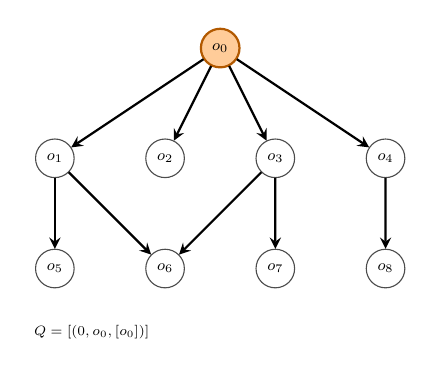
\begin{tikzpicture}[
    scale=0.7, transform shape,
    every node/.style={circle, draw, minimum size=7mm, font=\footnotesize\ttfamily},
    edge/.style={draw, ->, >=stealth, thick},
    current/.style={fill=orange!40, draw=orange!70!black, thick},
    default/.style={fill=white, draw=gray!60!black}
]
% Level 0
\node[current] (o0) at (3,4) {$o_0$};

% Level 1
\node[default] (o1) at (0,2) {$o_1$};
\node[default] (o2) at (2,2) {$o_2$};
\node[default] (o3) at (4,2) {$o_3$};
\node[default] (o4) at (6,2) {$o_4$};

% Level 2
\node[default] (o5) at (0,0) {$o_5$};
\node[default] (o6) at (2,0) {$o_6$};
\node[default] (o7) at (4,0) {$o_7$};
\node[default] (o8) at (6,0) {$o_8$};

% Edges from o0
\draw[edge] (o0) -- (o1);
\draw[edge] (o0) -- (o2);
\draw[edge] (o0) -- (o3);
\draw[edge] (o0) -- (o4);

% Edges from Level 1 to Level 2
\draw[edge] (o1) -- (o5);
\draw[edge] (o1) -- (o6);
\draw[edge] (o3) -- (o6);
\draw[edge] (o3) -- (o7);
\draw[edge] (o4) -- (o8);

% Queue annotation
\node[draw=none, rectangle, anchor=north west, align=left, font=\scriptsize, text=black]
    at (-0.5,-0.8) {$Q = [(0, o_0, [o_0])]$};
\end{tikzpicture}

        \label{fig:bfs_step_a}
    }
    \hfill
    \subfloat[Expand $o_0$ - candidates.]{
        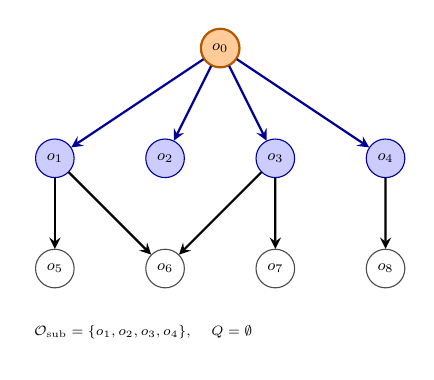
\begin{tikzpicture}[
    scale=0.7, transform shape,
    every node/.style={circle, draw, minimum size=7mm, font=\footnotesize\ttfamily},
    edge/.style={draw, ->, >=stealth, thick},
    candidedge/.style={draw, ->, >=stealth, thick, blue!60!black},
    current/.style={fill=orange!40, draw=orange!70!black, thick},
    candidate/.style={fill=blue!20, draw=blue!60!black},
    default/.style={fill=white, draw=gray!60!black}
]
% Level 0
\node[current] (o0) at (3,4) {$o_0$};

% Level 1 - all candidates (blue)
\node[candidate] (o1) at (0,2) {$o_1$};
\node[candidate] (o2) at (2,2) {$o_2$};
\node[candidate] (o3) at (4,2) {$o_3$};
\node[candidate] (o4) at (6,2) {$o_4$};

% Level 2
\node[default] (o5) at (0,0) {$o_5$};
\node[default] (o6) at (2,0) {$o_6$};
\node[default] (o7) at (4,0) {$o_7$};
\node[default] (o8) at (6,0) {$o_8$};

% Candidate edges from o0 (blue)
\draw[candidedge] (o0) -- (o1);
\draw[candidedge] (o0) -- (o2);
\draw[candidedge] (o0) -- (o3);
\draw[candidedge] (o0) -- (o4);

% Edges from Level 1 to Level 2 (default)
\draw[edge] (o1) -- (o5);
\draw[edge] (o1) -- (o6);
\draw[edge] (o3) -- (o6);
\draw[edge] (o3) -- (o7);
\draw[edge] (o4) -- (o8);

% Annotation
\node[draw=none, rectangle, anchor=north west, align=left, font=\scriptsize, text=black]
    at (-0.5,-0.8) {$\mathcal{O}_{\text{sub}} = \{o_1, o_2, o_3, o_4\}$, \quad $Q = \emptyset$};
\end{tikzpicture}

        \label{fig:bfs_step_b}
    }\\[2mm]
    \subfloat[Expand $o_0$ - selection.]{
        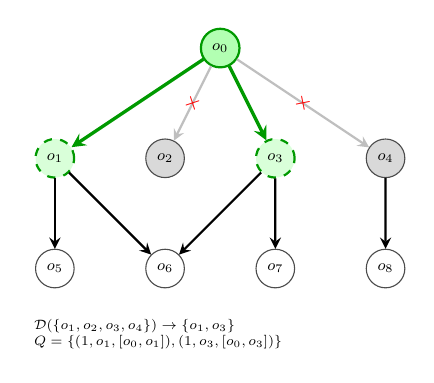
\begin{tikzpicture}[
    scale=0.7, transform shape,
    every node/.style={circle, draw, minimum size=7mm, font=\footnotesize\ttfamily},
    edge/.style={draw, ->, >=stealth, thick},
    selectedge/.style={draw, ->, >=stealth, very thick, green!60!black},
    rejectededge/.style={draw, ->, >=stealth, thick, gray!50,
        decoration={markings, mark=at position 0.5 with {\node[red, font=\scriptsize\bfseries, draw=none, fill=none] {$\times$};}},
        postaction={decorate}},
    processed/.style={fill=green!30, draw=green!60!black, thick},
    queued/.style={fill=green!15, draw=green!60!black, dashed, thick},
    rejected/.style={fill=gray!30, draw=gray!60!black},
    default/.style={fill=white, draw=gray!60!black}
]
% Level 0
\node[processed] (o0) at (3,4) {$o_0$};

% Level 1
\node[queued] (o1) at (0,2) {$o_1$};
\node[rejected] (o2) at (2,2) {$o_2$};
\node[queued] (o3) at (4,2) {$o_3$};
\node[rejected] (o4) at (6,2) {$o_4$};

% Level 2
\node[default] (o5) at (0,0) {$o_5$};
\node[default] (o6) at (2,0) {$o_6$};
\node[default] (o7) at (4,0) {$o_7$};
\node[default] (o8) at (6,0) {$o_8$};

% Selected edges from o0
\draw[selectedge] (o0) -- (o1);
\draw[selectedge] (o0) -- (o3);

% Rejected edges from o0
\draw[rejectededge] (o0) -- (o2);
\draw[rejectededge] (o0) -- (o4);

% Edges from Level 1 to Level 2 (default)
\draw[edge] (o1) -- (o5);
\draw[edge] (o1) -- (o6);
\draw[edge] (o3) -- (o6);
\draw[edge] (o3) -- (o7);
\draw[edge] (o4) -- (o8);

% Annotation
\node[draw=none, rectangle, anchor=north west, align=left, font=\scriptsize, text=black]
    at (-0.5,-0.8) {$\mathcal{D}(\{o_1,o_2,o_3,o_4\}) \to \{o_1,o_3\}$\\$Q = \{(1, o_1, [o_0,o_1]), (1, o_3, [o_0,o_3])\}$};
\end{tikzpicture}

        \label{fig:bfs_step_c}
    }
    \hfill
    \subfloat[Expand $o_1$ - candidates.]{
        \input{graphics/tikz/bfs_step_d.tex}
        \label{fig:bfs_step_d}
    }\\[2mm]
    \subfloat[Expand $o_1$ - selection.]{
        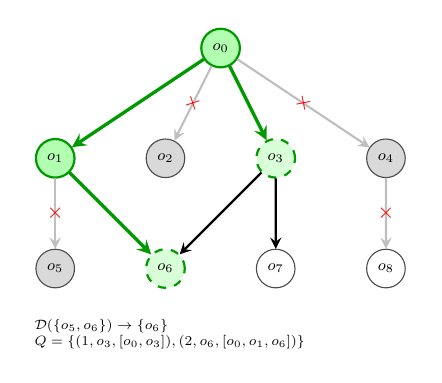
\begin{tikzpicture}[
    scale=0.7, transform shape,
    every node/.style={circle, draw, minimum size=7mm, font=\footnotesize\ttfamily},
    edge/.style={draw, ->, >=stealth, thick},
    selectedge/.style={draw, ->, >=stealth, very thick, green!60!black},
    rejectededge/.style={draw, ->, >=stealth, thick, gray!50,
        decoration={markings, mark=at position 0.5 with {\node[red, font=\scriptsize\bfseries, draw=none, fill=none] {$\times$};}},
        postaction={decorate}},
    processed/.style={fill=green!30, draw=green!60!black, thick},
    queued/.style={fill=green!15, draw=green!60!black, dashed, thick},
    rejected/.style={fill=gray!30, draw=gray!60!black},
    default/.style={fill=white, draw=gray!60!black}
]
% Level 0
\node[processed] (o0) at (3,4) {$o_0$};

% Level 1
\node[processed] (o1) at (0,2) {$o_1$};
\node[rejected] (o2) at (2,2) {$o_2$};
\node[queued] (o3) at (4,2) {$o_3$};
\node[rejected] (o4) at (6,2) {$o_4$};

% Level 2
\node[rejected] (o5) at (0,0) {$o_5$};
\node[queued] (o6) at (2,0) {$o_6$};
\node[default] (o7) at (4,0) {$o_7$};
\node[default] (o8) at (6,0) {$o_8$};

% Selected edges from o0
\draw[selectedge] (o0) -- (o1);
\draw[selectedge] (o0) -- (o3);

% Rejected edges from o0
\draw[rejectededge] (o0) -- (o2);
\draw[rejectededge] (o0) -- (o4);

% Edges from o1
\draw[selectedge] (o1) -- (o6);
\draw[rejectededge] (o1) -- (o5);

% Default edges from o3
\draw[edge] (o3) -- (o6);
\draw[edge] (o3) -- (o7);

% Rejected edge from o4
\draw[rejectededge] (o4) -- (o8);

% Annotation
\node[draw=none, rectangle, anchor=north west, align=left, font=\scriptsize, text=black]
    at (-0.5,-0.8) {$\mathcal{D}(\{o_5,o_6\}) \to \{o_6\}$\\$Q = \{(1, o_3, [o_0,o_3]), (2, o_6, [o_0,o_1,o_6])\}$};
\end{tikzpicture}

        \label{fig:bfs_step_e}
    }
    \hfill
    \subfloat[Expand $o_3$ - candidates.]{
        \input{graphics/tikz/bfs_step_f.tex}
        \label{fig:bfs_step_f}
    }\\[2mm]
    \subfloat[Expand $o_3$ - selection.]{
        \input{graphics/tikz/bfs_step_g.tex}
        \label{fig:bfs_step_g}
    }
    \hfill
    \subfloat[Termination.]{
        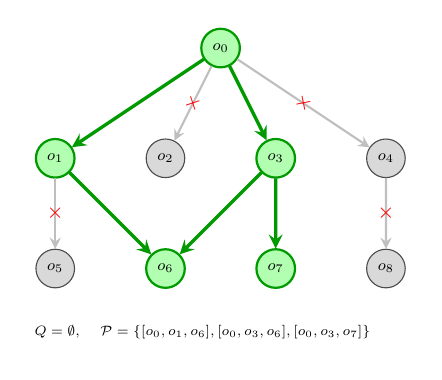
\begin{tikzpicture}[
    scale=0.7, transform shape,
    every node/.style={circle, draw, minimum size=7mm, font=\footnotesize\ttfamily},
    edge/.style={draw, ->, >=stealth, thick},
    selectedge/.style={draw, ->, >=stealth, very thick, green!60!black},
    rejectededge/.style={draw, ->, >=stealth, thick, gray!50,
        decoration={markings, mark=at position 0.5 with {\node[red, font=\scriptsize\bfseries, draw=none, fill=none] {$\times$};}},
        postaction={decorate}},
    processed/.style={fill=green!30, draw=green!60!black, thick},
    rejected/.style={fill=gray!30, draw=gray!60!black},
    default/.style={fill=white, draw=gray!60!black}
]
% Level 0
\node[processed] (o0) at (3,4) {$o_0$};

% Level 1
\node[processed] (o1) at (0,2) {$o_1$};
\node[rejected] (o2) at (2,2) {$o_2$};
\node[processed] (o3) at (4,2) {$o_3$};
\node[rejected] (o4) at (6,2) {$o_4$};

% Level 2
\node[rejected] (o5) at (0,0) {$o_5$};
\node[processed] (o6) at (2,0) {$o_6$};
\node[processed] (o7) at (4,0) {$o_7$};
\node[rejected] (o8) at (6,0) {$o_8$};

% Selected path edges
\draw[selectedge] (o0) -- (o1);
\draw[selectedge] (o0) -- (o3);
\draw[selectedge] (o1) -- (o6);
\draw[selectedge] (o3) -- (o6);
\draw[selectedge] (o3) -- (o7);

% Rejected edges
\draw[rejectededge] (o0) -- (o2);
\draw[rejectededge] (o0) -- (o4);
\draw[rejectededge] (o1) -- (o5);
\draw[rejectededge] (o4) -- (o8);

% Annotation
\node[draw=none, rectangle, anchor=north west, align=left, font=\scriptsize, text=black]
    at (-0.5,-0.8) {$Q = \emptyset$, \quad $\mathcal{P} = \{[o_0,o_1,o_6], [o_0,o_3,o_6], [o_0,o_3,o_7]\}$};
\end{tikzpicture}

        \label{fig:bfs_step_h}
    }

    \caption{Breadth-first traversal on an ontology DAG. Node states: \textcolor{orange!70!black}{orange} = expanding, \textcolor{blue!60!black}{blue} = candidate, \textcolor{green!60!black}{green solid} = processed, \textcolor{green!60!black}{green dashed} = queued, \textcolor{gray}{gray} = rejected. Rejected edges are marked with \textcolor{red}{$\times$}.}
    \label{fig:bfs_example}
\end{figure}

Figure~\ref{fig:bfs_example} illustrates the traversal on an ontology rooted at $o_0$ with two subclass layers. Consider annotating a column with header \textit{Fuel Type} from an energy dataset, with sample values such as \texttt{diesel}, \texttt{gasoline}, and \texttt{natural gas}. Let $l_{\max}=2$. The queue evolution is as follows:

\begin{enumerate}
    \item \textbf{Initialization (Fig.~\ref{fig:bfs_step_a}).}
    Initialize $\mathcal{P}\leftarrow\emptyset$ and $Q\leftarrow\emptyset$; enqueue $(0,o_0,[o_0])$.
    Queue state: $Q = [(0, o_0, [o_0])]$.

    \item \textbf{Expanding $o_0$ - candidate phase (Fig.~\ref{fig:bfs_step_b}).}
    Dequeue $(0,o_0,[o_0])$ and retrieve $\mathcal{O}_{\text{sub}}(o_0)=\{o_1,o_2,o_3,o_4\}$.
    These four subclasses (shown in blue) are passed to the decision module $\mathcal{D}$ for evaluation.

    \item \textbf{Expanding $o_0$ - selection result (Fig.~\ref{fig:bfs_step_c}).}
    The decision module returns $\mathcal{O}_{\text{sel}}=\{o_1,o_3\}$, rejecting $o_2$ and $o_4$.
    Enqueue $(1,o_1,[o_0,o_1])$ and $(1,o_3,[o_0,o_3])$.
    Queue state: $Q = [(1, o_1, [o_0,o_1]), (1, o_3, [o_0,o_3])]$.
    Selected nodes are shown with dashed green borders; rejected edges are marked with a red $\times$.

    \item \textbf{Expanding $o_1$ - candidate phase (Fig.~\ref{fig:bfs_step_d}).}
    Dequeue $(1,o_1,[o_0,o_1])$ and retrieve $\mathcal{O}_{\text{sub}}(o_1)=\{o_5,o_6\}$.
    These two subclasses (shown in blue) are passed to $\mathcal{D}$ for evaluation.
    Note that $o_3$ remains in the queue (dashed green), awaiting its turn.

    \item \textbf{Expanding $o_1$ - selection result (Fig.~\ref{fig:bfs_step_e}).}
    The decision module selects $\{o_6\}$ and rejects $o_5$.
    Enqueue $(2,o_6,[o_0,o_1,o_6])$.
    Queue state: $Q = [(1, o_3, [o_0,o_3]), (2, o_6, [o_0,o_1,o_6])]$.

    \item \textbf{Expanding $o_3$ - candidate phase (Fig.~\ref{fig:bfs_step_f}).}
    Dequeue $(1,o_3,[o_0,o_3])$ and retrieve $\mathcal{O}_{\text{sub}}(o_3)=\{o_6,o_7\}$.
    These two subclasses are passed to $\mathcal{D}$ for evaluation.
    Note that $o_6$ is already queued from $o_1$'s path, but is evaluated again under $o_3$'s context.

    \item \textbf{Expanding $o_3$ - selection result (Fig.~\ref{fig:bfs_step_g}).}
    The decision module selects both $\{o_6,o_7\}$.
    Enqueue $(2,o_6,[o_0,o_3,o_6])$ and $(2,o_7,[o_0,o_3,o_7])$.
    Queue state: $Q = [(2, o_6, [o_0,o_1,o_6]), (2, o_6, [o_0,o_3,o_6]), (2, o_7, [o_0,o_3,o_7])]$.

    \item \textbf{Termination (Fig.~\ref{fig:bfs_step_h}).}
    All remaining queue elements have depth $2=l_{\max}$, so the traversal finalizes each path without further expansion.
    The output is $\mathcal{P}=\{[o_0,o_1,o_6],\,[o_0,o_3,o_6],\,[o_0,o_3,o_7]\}$.
\end{enumerate}

The endpoint class $o_6$ appears under two distinct paths, reflecting that multiple higher-level categories can legitimately contextualize the same fine-grained label. The next section introduces ranking and consolidation strategies that control this multiplicity under scalability constraints.

\section{Chain-of-Thought Prompt Engineering}
\label{sec:prompt_engineering}

CTA in this pipeline relies on large language models (LLMs) to evaluate semantic compatibility between column evidence and ontology candidates. However, unconstrained LLM generations can be inconsistent and may produce labels not present in the ontology. The method therefore uses a structured prompting procedure that constrains the output space while eliciting intermediate reasoning steps, commonly known as chain-of-thought (CoT) prompting~\cite{wei2022chain}.

The prompt structure consists of three key components:

\begin{enumerate}
    \item \textbf{Role Definition:} The system message defines the LLM's role as an expert in semantic table annotation, with the goal of selecting the most appropriate ontology class for a given column based on the provided metadata.
    \item \textbf{Contextual Evidence:} To ground the model's decision, the prompt includes serialized table context (table name, column headers, and sample rows) formatted in Markdown. This provides the necessary evidence for disambiguating generic column names (e.g., distinguishing a numerical ``Capacity'' column as either electrical generation capacity or volume).
    \item \textbf{Constrained Candidate Set:} Crucially, the BFS traversal (Section~\ref{sec:bfs}) dynamically supplies a limited set of valid ontology classes ($\mathcal{O}_{\text{sub}}$) available at the current depth. The LLM is restricted to choosing from this set (or one of their ancestors), effectively transforming open-ended generation into a multiple-choice classification task grounded in the ontology.
\end{enumerate}

\paragraph{Implementation}
To improve the robustness of semantic judgments, the prompt separates the output into two logical blocks: a reasoning block and a final-answer block. Concretely, the prompt instructs the model to:
\begin{quote}
    ``First, output your reasoning enclosed in \texttt{<reasoning>...</reasoning>} tags. Then output the final answer enclosed in \texttt{<answer>...</answer>} tags.''
\end{quote}

The separation encourages an explicit justification of the relationship between column values and candidate classes before committing to a label. Within the \texttt{<reasoning>...</reasoning>} block, the model typically analyzes value patterns (e.g., \texttt{Solar} under a \texttt{Fuel} column suggests a renewable energy source) and contrasts candidate definitions. The extracted content of the \texttt{<answer>...</answer>} block is then parsed for the subsequent Ensemble Decision-Making phase.


\section{LLM-based Ensemble Decision-Making}
\label{sec:edm}

The decision module $\mathcal{D}$ in Algorithm~\ref{alg:bfs} determines which candidate classes to retain at each BFS level. Single LLM calls can be inconsistent, can hallucinate ontology-incompatible labels, and can be truncated by context-window limits. The pipeline therefore uses an \emph{Ensemble Decision-Making} (EDM) strategy that aggregates votes from multiple independent LLM agents to improve robustness.

The EDM module is governed by three hyperparameters: $\alpha$ (\emph{agents per class}) specifies how many independent agents evaluate each candidate class; $\beta$ (\emph{classes per agent}) bounds the workload assigned to a single agent; and $\theta \in [0,1]$ (\emph{consensus threshold}) sets the minimum vote ratio required for a class to be selected. The number of agents $n$ is computed dynamically to balance evaluation coverage and computational cost:
\begin{equation}
n = \max\left(\alpha,\, \left\lfloor\frac{|\hat{\mathcal{O}}| \cdot \alpha}{\beta}\right\rfloor + 1\right)
\label{eq:num_agents}
\end{equation}
This formula ensures that (i) at least $\alpha$ agents are available so each class can receive the required number of evaluations, and (ii) no agent is overloaded beyond $\beta$ classes on average.

\begin{algorithm}[htb]
\caption{LLM-based Ensemble Decision-Making}
\label{alg:edm}
\KwIn{
    Table context: name $t_n$, header $t_h$, sample rows $t_d$; \\
    Target column $c$; Candidate classes $\hat{\mathcal{O}}$; \\
    Agents per class $\alpha$; Classes per agent $\beta$; Consensus threshold $\theta$
}
\KwOut{Selected classes $\mathcal{O}_{\text{sel}} \subseteq \hat{\mathcal{O}}$}

\tcp{Step 1: Compute number of agents}
$n \leftarrow \max\bigl(\alpha,\, \lfloor|\hat{\mathcal{O}}| \cdot \alpha / \beta\rfloor + 1\bigr)$\;
Initialize assignment lists: $\text{assigned}[i] \leftarrow \emptyset$ for $i \in \{1, \ldots, n\}$\;
Initialize counters: $\text{votes}[o] \leftarrow 0$, $\text{seen}[o] \leftarrow 0$ for all $o \in \hat{\mathcal{O}}$\;

\BlankLine
\tcp{Step 2: Assign classes to agents}
\For{each class $o \in \hat{\mathcal{O}}$}{
    $\mathcal{I}_o \leftarrow$ randomly select $\min(\alpha, n)$ indices from $\{1, \ldots, n\}$\;
    \For{each $j \in \mathcal{I}_o$}{
        $\text{assigned}[j] \leftarrow \text{assigned}[j] \cup \{o\}$\;
        $\text{seen}[o] \leftarrow \text{seen}[o] + 1$\;
    }
}

\BlankLine
\tcp{Step 3: Query agents in parallel}
\ForPar{$i \leftarrow 1$ \KwTo $n$}{
    \If{$\text{assigned}[i] \neq \emptyset$}{
        $Q_i \leftarrow \textsc{GeneratePrompt}(t_n, t_h, t_d, c, \text{assigned}[i])$\;
        $R_i \leftarrow \textsc{LLMQuery}(Q_i)$\;
        $V_i \leftarrow \textsc{ParseAnswer}(R_i) \cap \text{assigned}[i]$\;
        \For{each $o \in V_i$}{
            $\text{votes}[o] \leftarrow \text{votes}[o] + 1$\;
        }
    }
}

\BlankLine
\tcp{Step 4: Apply consensus threshold}
$\mathcal{O}_{\text{sel}} \leftarrow \emptyset$\;
\For{each class $o \in \hat{\mathcal{O}}$}{
    \If{$\text{votes}[o] > 0$ \textbf{and} $\text{votes}[o] / \text{seen}[o] \geq \theta$}{
        $\mathcal{O}_{\text{sel}} \leftarrow \mathcal{O}_{\text{sel}} \cup \{o\}$\;
    }
}
\Return $\mathcal{O}_{\text{sel}}$\;
\end{algorithm}

Algorithm~\ref{alg:edm} proceeds in four phases. First, the number of agents $n$ is determined according to Equation~\ref{eq:num_agents}. Second, each candidate class $o \in \hat{\mathcal{O}}$ is randomly assigned to $\min(\alpha, n)$ agents; the counter $\text{seen}[o]$ records how many agents will evaluate class $o$. Third, all agents query the LLM in parallel with their assigned subsets of classes. Each agent constructs a prompt containing the table context (name, headers, sample rows), the target column, and its assigned candidates. The LLM response is parsed to extract the classes the agent deems relevant, and only classes within the agent's assignment are counted as votes. Finally, a class is selected if and only if it receives at least one positive vote and the ratio of votes to evaluating agents meets or exceeds the consensus threshold~$\theta$.

Agent queries are independent and therefore parallelizable: each agent issues an LLM request for its assigned subset of classes. With sufficient API concurrency, parallel execution reduces wall-clock latency from $O(n)$ sequential calls to $O(1)$ parallel calls. The additional constraint $\text{votes}[o] > 0$ in line~24 prevents vacuous acceptance when all evaluating agents abstain from voting for a particular class. Together, ontology-driven traversal, constrained prompting, and EDM yield a scalable CTA pipeline for heterogeneous energy tables.

% =============================================================================
% Chapter 5: System Architecture and Implementation
% =============================================================================

\chapter{System Architecture and Implementation}
\label{chap:system_architecture_implementation}

In this chapter, we present the system architecture and implementation of the semantic annotation platform. The architectural design prioritizes three fundamental principles: extensibility across various LLM providers, traceability of annotation decisions for auditability, and modularity to accommodate both batch experimentation and interactive analysis workflows.

% =============================================================================
% Section 5.1: System Overview
% =============================================================================

\section{System Overview}
\label{sec:system_overview}

% =============================================================================
% Section 5.2: Architecture
% =============================================================================

\subsection{Architecture}
\label{subsec:architecture}

We adopt a standard four-layer architecture, as illustrated in Figure~\ref{fig:system_overview}, to promote modularity and separation of concerns. The Web Interface enables user interaction and data visualization. The API Gateway serves as the communication bridge, handling request routing and command dispatching. Followed by the Core Engine, which encapsulates the primary computational modules, including data processing engine, the semantic annotation engine, and evaluation engine. Finally, the Data Storage manages the persistence of ontologies, tabular data, and system configurations. Architecturally, the system is deployed with a decoupled frontend and a unified backend service.

\begin{figure}[htbp]
    \centering
    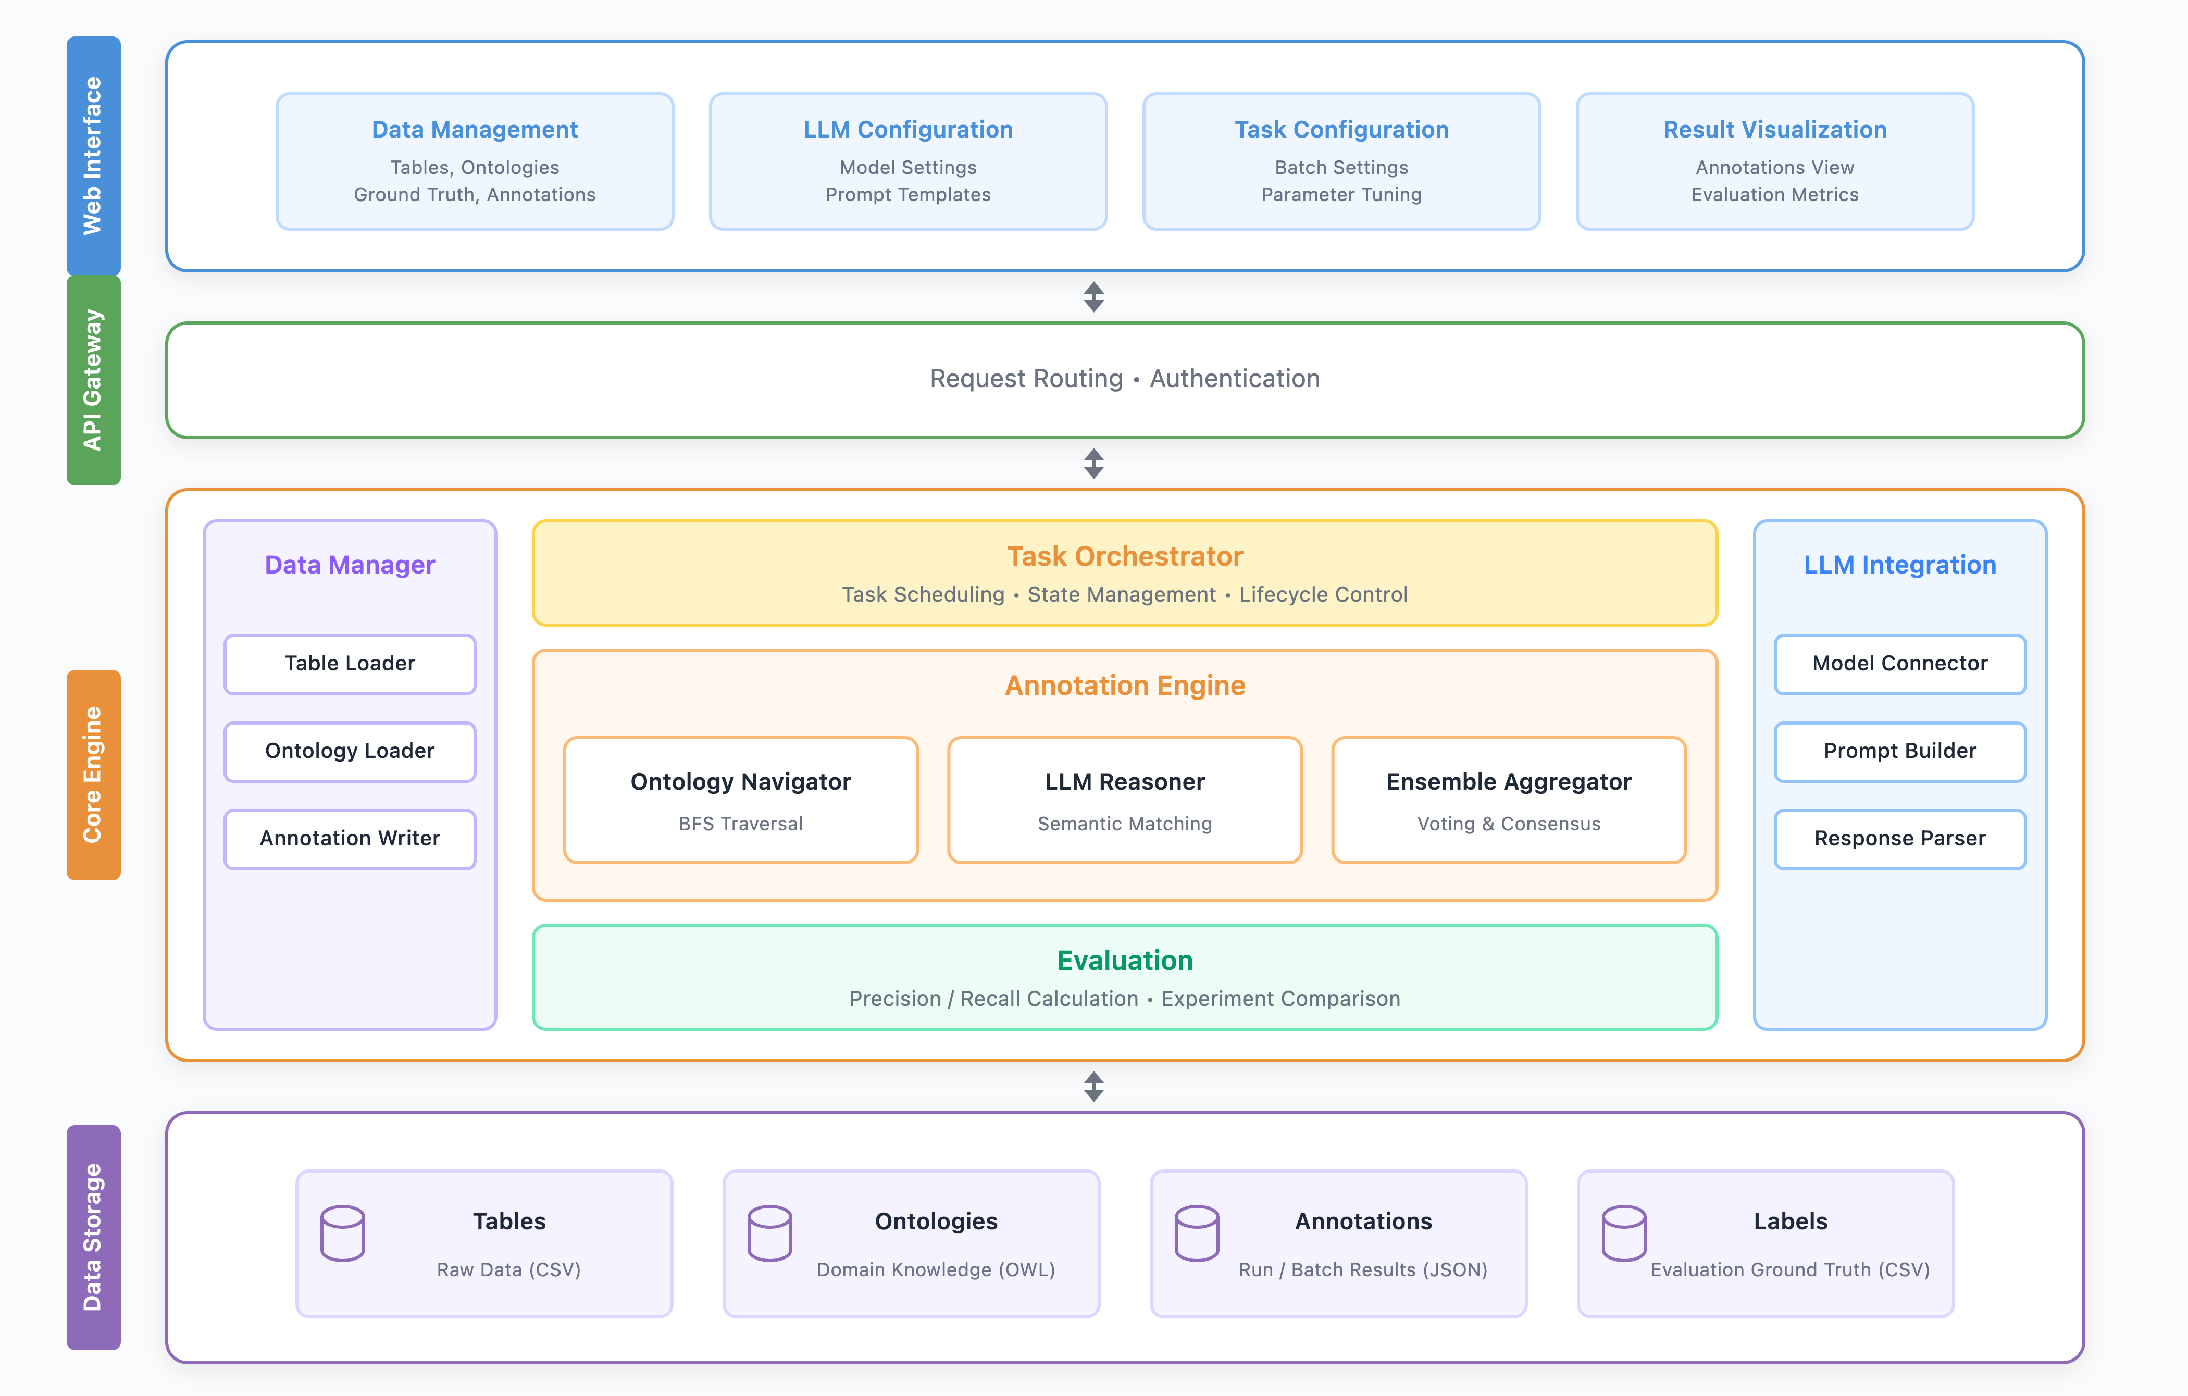
\includegraphics[width=\textwidth]{graphics/canvas/system_overview.pdf}
    \caption{System Architecture Overview. The architecture comprises four layers: Web Interface, API Gateway, Core Engine, and Data Layer. The Core Engine orchestrates the semantic annotation process through modules such as Task Orchestrator, Annotation Engine, and Evaluation.}
    \label{fig:system_overview}
\end{figure}

The architecture accommodates two complementary operational modes. \textbf{Interactive analysis} provides real-time monitoring and granular inspection of annotation decisions. Additionally, a Command Line Interface (CLI) provides additionaly a programmatic interface for \textbf{Batch processing} and automation, enabling high-throughput analysis across datasets and facilitating systematic empirical evaluation.

\subsection{Component Description}
\label{subsec:component_description}

The system architecture comprises four hierarchical layers, each encapsulating distinct functional responsibilities.

\paragraph{Web Interface.}
This layer exposes user-facing functionality through four modules: Data Management handles ingestion and organization of tables, ontologies, and ground truth artifacts; LLM Configuration manages model selection and prompt template specification; Task Configuration controls batch settings and algorithmic parameter tuning; Result Visualization renders annotations and evaluation metrics. Collectively, these modules constitute the primary interaction surface for end users.

\paragraph{API Gateway.}
This layer mediates request routing, concurrency management, and authentication. By abstracting communication between frontend and backend services, it ensures consistent request processing and decouples presentation logic from business logic.

\paragraph{Core Engine.}
This layer implements the primary computational logic through three integrated components. The Task Orchestrator manages scheduling, state transitions, and lifecycle control. The Annotation Engine comprises three submodules: the Ontology Navigator for hierarchical traversal, the LLM Reasoner for semantic matching, and the Ensemble Aggregator for vote consolidation. The Evaluation Module computes precision, recall, and related metrics against ground truth annotations. This layer represents the algorithmic core of the platform.

\paragraph{Data Layer.}
This layer persists four categories of artifacts: Tables containing raw input data, Ontologies encoding domain knowledge structures, Annotations storing run and batch results, and Ground Truth providing evaluation labels. This separation ensures referential integrity and supports reproducible experimentation.

\subsection{Data Flow}
\label{subsec:data_flow}

The annotation workflow adheres to a structured artifact lifecycle, ensuring traceability and reproducibility throughout execution.

\begin{enumerate}
    \item \textbf{Ontology Loading.} The ontology file undergoes parsing and transformation into a Directed Acyclic Graph (DAG) representation. The resulting artifact is registered with version metadata to ensure semantic stability across experiments.

    \item \textbf{Table Ingestion.} Input tables are parsed to produce Column Context objects encapsulating headers, type hints, and representative sample values. This normalization step isolates data heterogeneity from downstream annotation logic.

    \item \textbf{Annotation Execution.} The Breadth-first Search (BFS) executor traverses the ontology hierarchy, invoking the Ensemble Decision Making (EDM) module at each depth level to filter candidate classes. When multiple branches survive traversal, path selection is determined by accumulated branch scores.

    \item \textbf{Result Persistence.} Predictions are serialized alongside comprehensive execution traces capturing prompts, responses, and intermediate decisions. This linkage enables post-hoc analysis and error attribution.

    \item \textbf{Evaluation.} The evaluation module computes performance metrics by comparing predictions against ground truth annotations, generating the summary statistics requisite for empirical benchmarking.
\end{enumerate}

% =============================================================================
% Section 5.2: Core Components
% =============================================================================

\section{Core Components}
\label{sec:core_components}

\subsection{Ontology Management}
\label{subsec:ontology_management}

The Ontology Management module transforms static ontology artifacts into an optimized internal representation that facilitates efficient querying during annotation.

\paragraph{Loading and Parsing.}
The platform supports standard Semantic Web serializations, including RDF/XML and Turtle formats and OWL 2.0. During ingestion, the parser systematically extracts classes identified by Internationalized Resource Identifiers (IRIs), human-readable labels and descriptions, and hierarchical relationships based on the \texttt{rdfs:subClassOf} relation. Notably, anonymous classes and complex OWL restrictions are explicitly filtered to maintain a strict DAG structure comprising only named classes, which reduces computational complexity while preserving the taxonomic backbone essential for traversal.

\paragraph{DAG Construction and Caching.}
Following parsing, the ontology is formalized as a directed acyclic graph (DAG) $G=(V,E)$, where edge $(u,v) \in E$ indicates that $v$ is a subclass of $u$. To support efficient traversal, the system materializes two adjacency caches:
\begin{itemize}
    \item \textbf{Children Cache:} $\text{children}[u] = \{ v \mid (u,v) \in E \}$
    \item \textbf{Parents Cache:} $\text{parents}[v] = \{ u \mid (u,v) \in E \}$
\end{itemize}

The platform designates \texttt{owl:Thing} as the unique traversal root, ensuring consistency with standard OWL semantics. Furthermore, the DAG construction phase enforces structural integrity through active cycle detection. Although subclass relations are semantically intended to be acyclic, modeling errors occasionally introduce cycles that would cause infinite loops during traversal. When detected, cycles are resolved deterministically by pruning the edge that completes the cycle, thereby guaranteeing the DAG property required for BFS termination.

\subsection{Table Processing}
\label{subsec:table_processing}

The Table Processing module serves as the intermediary between raw tabular inputs and the annotation engine, producing compact, LLM-ready representations.

\paragraph{Input Formats and Parsing.}
The platform supports standard domain table formats, including CSV and Excel exports. The parser converts files into an internal dataframe representation preserving column headers as raw strings, cell values with explicit handling of missing data, and fundamental schema metadata. Given that domain tables frequently exhibit inconsistent encodings, such as mixed numeric and string fields or sentinel values, the parsing logic prioritizes robustness over strict type enforcement. When type inference is ambiguous, the system defaults to a mixed object type, delegating semantic disambiguation to the downstream LLM.

\paragraph{Column Context Extraction.}
For each column $c_i$, the module constructs a Column Context Object comprising three elements:
\begin{description}
    \item[Header:] The original column name, serving as the primary semantic signal.
    \item[Type Hint:] A coarse data type category (Numeric, Categorical, Timestamp, Boolean, or Mixed) derived through heuristic inference.
    \item[Sample Values:] A bounded set of representative values selected according to a configurable sampling policy.
\end{description}

The sampling step addresses a critical constraint: domain tables often contain extensive time series, rendering full-column inclusion token-prohibitive. Consequently, the platform enforces a hard cap on sampled values per column and applies consistent filtering rules to exclude nulls and whitespace, providing sufficient evidence for semantic disambiguation while maintaining predictable token consumption.

\paragraph{Batch Processing Support.}
The module provides batch-oriented utilities essential for dataset-scale experiments. These include dataset ingestion across table collections, progress reporting via the unified API, failure isolation to prevent individual parsing errors from aborting entire experiments, and deterministic outputs guaranteeing bit-identical context objects across repeated executions. This determinism constitutes a prerequisite for controlled comparative experiments.

\subsection{Annotation Engine}
\label{subsec:annotation_engine}

The Annotation Engine serves as the operational core executing the workflow. It orchestrates interactions among the ontology DAG, column contexts, and the LLM client abstraction layer.

\paragraph{Execution Workflow.}
At runtime, the engine adheres to a deterministic execution protocol. First, it initializes the run context by loading the target ontology snapshot structurally rooted at \texttt{owl:Thing}. Subsequently, for each column, the engine initiates traversal at the root and iterates level-by-level: valid child nodes are retrieved via the children cache, the EDM module evaluates the candidate set and returns survivors, and new branches are enqueued for expansion. Traversal terminates when no survivors remain or the configured depth limit is reached. Finally, when multiple branches survive, the engine selects the optimal path based on the highest accumulated branch score. Given fixed inputs and deterministic provider behavior, the control flow remains strictly reproducible.

\paragraph{Result Caching.}
To mitigate redundant computation during iterative experimentation, the engine implements caching at the final result level, mapping configurations to predicted paths. However, cache reuse is strictly validated: results are deemed reusable only when the ontology snapshot, prompt template identifier, model provider settings, and EDM parameters match the current configuration exactly.

\paragraph{Error Handling and Retry Logic.}
Given the engine's dependency on external LLM APIs, robust error handling is fundamental. The executor encapsulates provider interactions within a reliability layer featuring exception capture for request-level failures, exponential backoff strategies for transient errors, and graceful degradation that records failures in the execution trace rather than aborting the entire annotation run. All exceptions are logged with precise timestamps and provider identifiers, facilitating diagnosis of partial failures in runs involving hundreds of API calls.

\subsection{Evaluation Module}
\label{subsec:evaluation_module}

The Evaluation Module performs systematic assessment by computing node-level and path-level metrics against ground truth annotations. Specifically, it calculates precision, recall, and F1 scores, aggregating results across datasets. By integrating evaluation as a first-class pipeline component, the system ensures that experimental results remain reproducible and directly comparable.

% =============================================================================
% Section 5.3: Traceability and Observability
% =============================================================================

\section{Traceability and Observability}
\label{sec:traceability}

A central design tenet of the platform is that annotation results must not be treated as opaque outputs; rather, they constitute verifiable decisions subject to inspection, reproduction, and audit. Since the system relies on external LLM providers and stochastic inference, traceability is implemented as a first-class concern.

\subsection{Execution Logging}
\label{subsec:execution_logging}

For each column and at every BFS depth level, the system persists a granular log entry capturing five dimensions:
\begin{itemize}
    \item \textbf{Context:} The column identifier and its extracted context (name, type, samples).
    \item \textbf{State:} The set of candidate ontology classes considered at that level.
    \item \textbf{Decisions:} The EDM outcomes, including vote counts, selected survivors, and support scores.
    \item \textbf{Evidence:} The verbatim prompts transmitted to the provider and raw responses received.
    \item \textbf{Metadata:} Operational metrics including request latency.
\end{itemize}

Notably, token usage data is recorded only when explicitly provided by the runtime. If the provider does not return usage statistics, the field is recorded as null. This policy prevents conflation of precise provider-reported costs with local approximations, ensuring data integrity for downstream cost analyses.

\subsection{Real-Time Monitoring}
\label{subsec:real_time_monitoring}

Long-running annotation tasks expose their state via Server-Sent Events (SSE). The executor streams structured events including:
\begin{itemize}
    \item \textbf{Progress:} Current completion status (processed columns versus total).
    \item \textbf{Intermediate Results:} Predicted paths for columns immediately upon completion.
    \item \textbf{Operational Status:} Warnings, errors, and retry notifications.
    \item \textbf{Completion Summaries:} Aggregate runtime metrics and final status.
\end{itemize}

This streaming architecture enables the Web UI to reflect system behavior dynamically without polling. Consequently, users can identify configuration issues---such as overly strict thresholds yielding empty selections---while jobs remain in progress. This immediate feedback loop significantly accelerates iterative refinement.

% =============================================================================
% Section 5.4: Implementation Details
% =============================================================================

\section{Implementation Details}
\label{sec:implementation}

\subsection{Technology Stack}
\label{subsec:technology_stack}

\paragraph{Backend Infrastructure.}
The backend logic is implemented in Python, selected for its dominant ecosystem in data processing, semantic web tooling (e.g., \texttt{rdflib}), and machine learning integration. The system exposes functionality through an asynchronous web service built upon FastAPI, which provides strict schema validation via Pydantic models, native support for asynchronous concurrency enabling long-running jobs and real-time SSE streaming, and ASGI compliance facilitating deployment across diverse environments.

\paragraph{Frontend Interface.}
The interactive user interface is constructed using Next.js, a React-based framework enabling a modern single-page application experience. The frontend manages configuration workflows, provides real-time observability via SSE subscription, and offers specialized views for auditing intermediate decisions.

\paragraph{Data Persistence.}
To support auditability and portability, the platform adopts a lightweight persistence model centered on a file-based JSON Registry. Rather than relying on a database management system, key artifacts are persisted as structured files. The registry manages ontology snapshots with unique identifiers and parsing statistics, dataset configurations recording file paths and normalization rules, experiment manifests capturing provider settings and EDM parameters, and execution traces containing full logs of prompts, responses, and latency. The file-centric approach facilitates easy export and sharing of experimental data, enabling researchers to reproduce results independent of the original runtime environment.

\subsection{User Interfaces}
\label{subsec:user_interfaces}

\subsubsection{Command-Line Interface}
\label{subsubsec:cli}

The Command-Line Interface (CLI) serves as a robust control layer designed to facilitate reproducible experimentation and automated workflow orchestration.
In contrast to manual execution, the CLI enables precise configuration of the semantic annotation lifecycle through a modular command structure.
The system exposes three primary directives:

\begin{itemize}
    \item \textbf{Annotation Execution:} \\ 
    \texttt{saed-run --table --ontology --mode --output-dir} \\
    Initiates the annotation process for a single table, supporting detailed configuration of the reasoning mode and prompt strategy.
    \item \textbf{Batch Processing:} \\
    \texttt{saed-run-batch --config batch.yaml} \\
    Orchestrates parallel execution across multiple datasets, enabling systematic comparative experiments defined via declarative configuration files.
    \item \textbf{Evaluation:} \\
    \texttt{saed-eval <batch\_file> --labels <ground\_truth> --format all} \\
    Computes comprehensive performance metrics, including node-level and path-level precision, recall, and F1 scores.
\end{itemize}

The system employs a file-system-based synchronization mechanism for Ontology and Dataset registries, eliminating the need for explicit registration commands.
Table~\ref{tab:cli_parameters} strictly defines the configurable parameters for the execution runtime.

\begin{table}[htbp]
    \centering
    \caption{Key CLI parameters for the execution runtime.}
    \label{tab:cli_parameters}
    \renewcommand{\arraystretch}{1.2}
    \small
    \begin{tabular}{lp{3cm}p{7cm}}
        \toprule
        \textbf{Parameter} & \textbf{Category} & \textbf{Description} \\
        \midrule
        \texttt{--table}      & Data      & Registry ID or filename of the target table \\
        \texttt{--ontology}   & Data      & Registry ID or filename of the domain ontology \\
        \texttt{--mode}       & Algorithm & Decision mode (\texttt{single} or \texttt{edm}) \\
        \texttt{--max\_depth} & Algorithm & Maximum traversal depth for the BFS strategy \\
        \texttt{--provider}   & Model     & LLM backend service (overrides config) \\
        \texttt{--output-dir} & System    & Directory path for persisting run artifacts \\
        \bottomrule
    \end{tabular}
\end{table}

This architecture ensures that all experiments are idempotent and fully reproducible.
The batch processor further supports shell-level orchestration, facilitating the migration of experimental setups between diverse computational environments while respecting provider rate limits.

\subsubsection{Web Interface}
\label{subsubsec:web_interface}

While the CLI optimizes for high-throughput batch experimentation, the Web Interface addresses the complementary requirement for interactive execution and granular inspection. The graphical interface enables researchers to scrutinize decision boundaries and trace reasoning paths for specific column mappings, supporting seamless transition between parameter tuning and validation.

\subsection{API Design}
\label{subsec:api_design}

The platform exposes its core functionality through a compact HTTP API, employing two distinct interaction paradigms to balance control and observability.

\paragraph{RESTful Endpoints.}
The REST API adheres to a resource-oriented design philosophy, minimizing client-side complexity while providing full access to the system's capabilities:
\begin{itemize}
    \item \texttt{POST /api/runs} -- Submit a new annotation job. Returns a unique run identifier upon successful initialization.
    \item \texttt{GET /api/runs/\{run\_id\}} -- Query the current status, progress counters, and configuration metadata of a specific run.
    \item \texttt{POST /api/evaluations} -- Compute performance metrics for a completed batch against ground truth references.
    \item \texttt{GET /api/evaluations/compare} -- Comparative analysis of multiple runs to benchmark different configurations.
\end{itemize}

\paragraph{Real-Time Streaming via SSE.}
For long-running annotation tasks, polling REST endpoints introduces unnecessary latency and inefficiency.
Therefore, the backend exposes a dedicated streaming endpoint \texttt{GET /api/runs/\{run\_id\}/stream}, emitting structured JSON events conforming to the \texttt{text/event-stream} content type.
Events include fine-grained progress updates (e.g., \texttt{column\_start}, \texttt{step}), intermediate results, and completion summaries.

Server-Sent Events (SSE) were selected over WebSockets due to their lightweight implementation profile and native browser support for unidirectional server-to-client updates.
This design aligns with the annotation execution model, where the client primarily consumes status updates.
Combined with comprehensive execution logging, this API architecture ensures robust observability, enabling users to initiate jobs programmatically via REST and monitor their evolution in real-time.



\chapter{Evaluation}
\label{chap:evaluation}

\section{Experimental Setup}
\label{sec:experimental_setup}

We evaluate the platform and the algorithm through a controlled factorial experiment that varies three system dimensions: \textbf{LLM providers} (commercial vs.\ open-source models), \textbf{prompting strategies} (direct vs.\ chain-of-thought), and \textbf{decision modes} (single-agent vs.\ ensemble). All experiments use the same dataset and target ontology and follow a breadth-first traversal rooted at \texttt{owl:Thing}; only the configuration variables defined below are varied.

% -----------------------------------------------------------------------------
% Subsection: Dataset
% -----------------------------------------------------------------------------
\subsection{Dataset}
\label{subsec:dataset}

\paragraph{Tables.}
The evaluation is conducted on a domain-specific benchmark comprises real-world tabular data collected from heterogeneous building management systems and energy audits. The benchmark consists of 47 distinct tables containing a total of 431 columns. Each column is treated as an independent semantic annotation instance. Domain experts assign each column a terminal BEO class; the corresponding \emph{root-to-leaf} ontology path serves as the \textit{gold standard} for both node-level and path-level evaluation.

\paragraph{Ontology.}
The experiments utilize the \textbf{Building Energy Ontology (BEO)} as the target concept space. This ontology comprises 602 classes organized into a hierarchy with a maximum depth of 8. The class hierarchy is formally represented as a Directed Acyclic Graph (DAG) derived principally from \texttt{rdfs:subClassOf} relations. All traversals originate from the universal root \texttt{owl:Thing}; no synthetic super-roots are introduced. During annotation, candidate classes at depth $d$ are generated strictly by expanding the children of the current frontier nodes. Figure~\ref{fig:ontology_example} illustrates a representative fragment of the BEO ontology structure.

% FIGURE: Ontology Example
\begin{figure}[htbp]
    \centering
    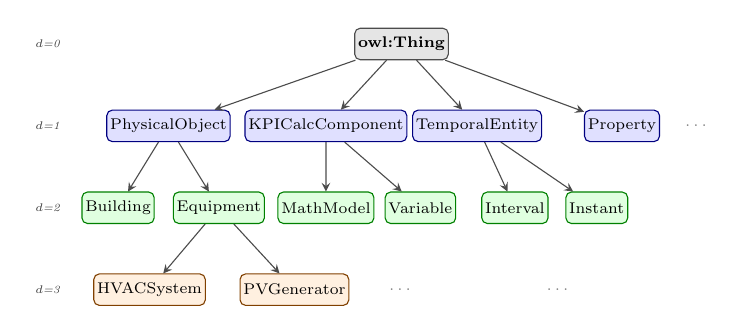
\begin{tikzpicture}[
    scale=0.8, transform shape,
    every node/.style={font=\scriptsize},
    class/.style={rectangle, rounded corners=2pt, draw, minimum height=5mm, align=center, inner sep=1.5pt},
    root/.style={class, fill=gray!20, draw=gray!60!black, font=\scriptsize\bfseries},
    level1/.style={class, fill=blue!12, draw=blue!50!black},
    level2/.style={class, fill=green!12, draw=green!50!black},
    level3/.style={class, fill=orange!12, draw=orange!50!black},
    edge/.style={draw, ->, >=stealth, gray!60!black},
    depthlabel/.style={font=\tiny\itshape, text=gray!50!black}
]

% Depth labels on the left (moved further left)
\node[depthlabel, anchor=east] at (-0.8, 0) {$d$=0};
\node[depthlabel, anchor=east] at (-0.8, -1.3) {$d$=1};
\node[depthlabel, anchor=east] at (-0.8, -2.6) {$d$=2};
\node[depthlabel, anchor=east] at (-0.8, -3.9) {$d$=3};

% Level 0: Root
\node[root] (thing) at (4.5, 0) {owl:Thing};

% Level 1: Top-level categories (from BEO ontology)
\node[level1] (physical) at (0.8, -1.3) {PhysicalObject};
\node[level1] (kpicomp) at (3.3, -1.3) {KPICalcComponent};
\node[level1] (temporal) at (5.7, -1.3) {TemporalEntity};
\node[level1] (property) at (8, -1.3) {Property};

% Level 2: Sub-categories
\node[level2] (building) at (0, -2.6) {Building};
\node[level2] (equipment) at (1.6, -2.6) {Equipment};
\node[level2] (mathmodel) at (3.3, -2.6) {MathModel};
\node[level2] (variable) at (4.8, -2.6) {Variable};
\node[level2] (interval) at (6.3, -2.6) {Interval};
\node[level2] (instant) at (7.6, -2.6) {Instant};

% Level 3: Leaf classes (moved apart to avoid overlap)
\node[level3] (hvac) at (0.5, -3.9) {HVACSystem};
\node[level3] (pv) at (2.8, -3.9) {PVGenerator};

% Edges from root
\draw[edge] (thing) -- (physical);
\draw[edge] (thing) -- (kpicomp);
\draw[edge] (thing) -- (temporal);
\draw[edge] (thing) -- (property);

% Edges from Level 1
\draw[edge] (physical) -- (building);
\draw[edge] (physical) -- (equipment);
\draw[edge] (kpicomp) -- (mathmodel);
\draw[edge] (kpicomp) -- (variable);
\draw[edge] (temporal) -- (interval);
\draw[edge] (temporal) -- (instant);

% Edges from Level 2
\draw[edge] (equipment) -- (hvac);
\draw[edge] (equipment) -- (pv);

% Ellipsis nodes to indicate more classes
\node[font=\scriptsize, text=gray] at (4.5, -3.9) {$\cdots$};
\node[font=\scriptsize, text=gray] at (7, -3.9) {$\cdots$};
\node[font=\scriptsize, text=gray] at (9.2, -1.3) {$\cdots$};

\end{tikzpicture}

    \caption[BEO ontology structure]{A fragment of the BEO ontology hierarchy. The ontology is organized as a DAG rooted at \texttt{owl:Thing}, with domain-specific classes such as \texttt{Equipment}, \texttt{Measurement}, and \texttt{TemporalEntity} at intermediate levels.}
    \label{fig:ontology_example}
\end{figure}

% -----------------------------------------------------------------------------
% Subsection: Preprocessing
% -----------------------------------------------------------------------------
\subsection{Preprocessing}
\label{subsec:eval_preprocessing}

To isolate the behaviour of the annotation logic, the system encodes each column using a uniform context representation comprising three elements: the original column header string, a coarse inferred type hint (e.g., Numeric, String), and a set of representative sample values selected using a \textit{Head-K} policy with $k=5$. These features form the only table-derived input to the LLM-based decision modules. No table-level descriptions or external knowledge-base signals are injected, so the evaluation reflects reasoning from column-local evidence alone.

% -----------------------------------------------------------------------------
% Subsection: Evaluation Metrics
% -----------------------------------------------------------------------------
\subsection{Evaluation Metrics}
\label{sec:eval_metrics}

We evaluate annotation quality at two granularities using set-based precision, recall, and F$_1$ metrics at node level and path level. Let $\mathcal{D} = \{(x_i, Y_i, \hat{Y}_i)\}_{i=1}^{N}$ denote the evaluation set, where $x_i$ is a column, $Y_i$ is the set of ground-truth ontology paths, and $\hat{Y}_i$ is the set of predicted paths. Each path is a sequence of class labels from root to leaf (e.g., $\langle\texttt{Thing}, \texttt{Measurement}, \texttt{Currency}\rangle$).

\paragraph{Node-Level Metrics.}
Node-level evaluation assesses the coverage of individual ontology classes along the predicted paths. We define a flattening operator $\mathcal{N}(\cdot)$ that extracts all unique class labels from a set of paths:
\begin{equation}
    \mathcal{N}(Y) = \bigcup_{p \in Y} \{c : c \in p\}
\end{equation}
For each instance $i$, we compute confusion counts over the flattened class sets:
\begin{align}
    \text{TP}_i &= |\mathcal{N}(\hat{Y}_i) \cap \mathcal{N}(Y_i)|, \quad
    \text{FP}_i = |\mathcal{N}(\hat{Y}_i) \setminus \mathcal{N}(Y_i)|, \quad
    \text{FN}_i = |\mathcal{N}(Y_i) \setminus \mathcal{N}(\hat{Y}_i)|
\end{align}

\paragraph{Path-Level Metrics.}
Path-level evaluation applies \textbf{strict path equality}: a prediction is correct only if the entire class sequence matches the ground truth exactly. Two paths $p$ and $q$ are equal iff $|p| = |q|$ and $p_j = q_j$ for all $j \in \{1, \ldots, |p|\}$. Confusion counts are computed directly on path sets:
\begin{align}
    \text{TP}_i &= |\hat{Y}_i \cap Y_i|, \quad
    \text{FP}_i = |\hat{Y}_i \setminus Y_i|, \quad
    \text{FN}_i = |Y_i \setminus \hat{Y}_i|
\end{align}
Under this strict criterion, a single incorrect branch decision at any traversal depth invalidates the entire path.

\paragraph{Aggregation: Micro- vs.\ Macro-Averaging.}

We report both micro- and macro-averaged metrics to characterize performance under class imbalance. 

\textbf{Micro-averaging} aggregates confusion counts across all instances before computing metrics, thereby weighting each prediction equally:
\begin{equation}
    P_{\mu} = \frac{\sum_{i=1}^{N} \text{TP}_i}{\sum_{i=1}^{N} (\text{TP}_i + \text{FP}_i)}, \quad
    R_{\mu} = \frac{\sum_{i=1}^{N} \text{TP}_i}{\sum_{i=1}^{N} (\text{TP}_i + \text{FN}_i)}, \quad
    F_{1,\mu} = \frac{2 P_{\mu} R_{\mu}}{P_{\mu} + R_{\mu}}
\end{equation}

\textbf{Macro-averaging} computes per-instance metrics and averages uniformly, giving equal weight to each column regardless of path cardinality:
\begin{equation}
    P_i = \frac{\text{TP}_i}{\text{TP}_i + \text{FP}_i}, \quad
    R_i = \frac{\text{TP}_i}{\text{TP}_i + \text{FN}_i}, \quad
    F_{1,i} = \frac{2 P_i R_i}{P_i + R_i}
\end{equation}
\begin{equation}
    P_M = \frac{1}{N}\sum_{i=1}^{N} P_i, \quad
    R_M = \frac{1}{N}\sum_{i=1}^{N} R_i, \quad
    F_{1,M} = \frac{1}{N}\sum_{i=1}^{N} F_{1,i}
\end{equation}

The BEO benchmark exhibits a long-tailed class distribution: a small number of frequent classes account for a disproportionate share of annotations, while many classes appear rarely. Micro-averaging tends to reflect performance on frequent classes, whereas macro-averaging penalizes errors on minority classes more heavily. We report both to provide a complete picture: micro-F$_1$ indicates aggregate predictive utility, while macro-F$_1$ reveals robustness across the class distribution. 

We additionally report total time as a deployment-relevant indicator of end-to-end efficiency.

% -----------------------------------------------------------------------------
% Subsection: Experiment Matrix
% -----------------------------------------------------------------------------
\subsection{Experiment Matrix}
\label{subsec:experiment_matrix}

We evaluate 8 distinct configurations defined by the Cartesian product of three variables:
\begin{equation}
    \text{Config} \in \text{Provider} \times \text{Prompt} \times \text{Decision Mode}
\end{equation}
where:
\begin{itemize}
    \item $\text{Provider} \in \{ \texttt{Azure (GPT-4.1)}, \texttt{Ollama (GPT-OSS:20b)} \}$
    \item $\text{Prompt} \in \{ \texttt{Direct}, \texttt{CoT} \}$
    \item $\text{Decision Mode} \in \{ \texttt{Single}, \texttt{EDM} \}$
\end{itemize}

\paragraph{Prompting Styles.}
\textbf{Direct} prompting instructs the model to return a classification decision without explicit intermediate reasoning. \textbf{Chain-of-Thought (CoT)} prompting requires the model to produce a brief reasoning trace before outputting the final decision.

\paragraph{Decision Modes.}
Under \textbf{Single} mode, decisions are rendered by a single LLM judgment per candidate set. Under \textbf{EDM} mode, decisions are produced via multi-agent voting with fixed hyperparameters: $\beta=30$ (classes per agent), $\alpha=3$ (agents per class), and $\theta=0.8$ (consensus threshold).

\paragraph{Execution Protocol.}
To minimize uncontrolled variance, all runs utilize a fixed temperature setting kept constant across providers and prompt styles. The pipeline operates sequentially: within a run, columns and EDM agent calls are executed with an effective parallelism of 1. Consequently, the reported total time represents wall-clock runtime per experiment run, encompassing API latency and orchestration overhead. Table~\ref{tab:experiment_matrix} summarizes all eight configurations.

% TABLE: Experiment Matrix
\begin{table}[htbp]
    \centering
    \caption{Experiment configuration matrix.}
    \label{tab:experiment_matrix}
    \renewcommand{\arraystretch}{1.2}
    \small
    \begin{tabular}{lcccc}
        \toprule
        \textbf{Run Name} & \textbf{Provider} & \textbf{Prompt} & \textbf{Mode} & \makecell{\textbf{EDM Params} \\ ($\beta/\alpha/\theta$)} \\
        \midrule
        \texttt{azure\_direct\_single} & Azure (GPT-4.1) & Direct & Single & -- \\
        \texttt{azure\_direct\_edm} & Azure (GPT-4.1) & Direct & EDM & 30/3/0.8 \\
        \texttt{azure\_cot\_single} & Azure (GPT-4.1) & CoT & Single & -- \\
        \texttt{azure\_cot\_edm} & Azure (GPT-4.1) & CoT & EDM & 30/3/0.8 \\
        \texttt{ollama\_direct\_single} & Ollama (GPT-OSS:20b) & Direct & Single & -- \\
        \texttt{ollama\_direct\_edm} & Ollama (GPT-OSS:20b) & Direct & EDM & 30/3/0.8 \\
        \texttt{ollama\_cot\_single} & Ollama (GPT-OSS:20b) & CoT & Single & -- \\
        \texttt{ollama\_cot\_edm} & Ollama (GPT-OSS:20b) & CoT & EDM & 30/3/0.8 \\
        \bottomrule
    \end{tabular}
\end{table}

% =============================================================================
% Section: Main Results
% =============================================================================
\section{Main Results}
\label{sec:main_results}

Table~\ref{tab:main_results} summarises the quantitative performance of the eight configurations defined in Section~\ref{sec:experimental_setup}. We report micro- and macro-averaged node- and path-level F$_1$ together with end-to-end wall-clock runtime. Under strict path equality, a single mistake at any depth invalidates the entire prediction, which systematically lowers path-level scores relative to node-level scores; the following subsections analyse the drivers of this gap.

% TABLE: Main Results
\begin{table}[htbp]
    \centering
    \caption{Main experimental results across 8 configurations. Node and path metrics are reported as F$_1$ scores (\%). Runtime is reported in seconds and minutes.}
    \label{tab:main_results}
    \renewcommand{\arraystretch}{1.2}
    \setlength{\tabcolsep}{4pt}
    \small
    \begin{tabular}{lcccccc}
        \toprule
        \multirow{2}{*}{\textbf{Configuration}} & \multicolumn{2}{c}{\textbf{Node F$_1$ (\%)}} & \multicolumn{2}{c}{\textbf{Path F$_1$ (\%)}} & \multicolumn{2}{c}{\textbf{Runtime}} \\
        \cmidrule(lr){2-3} \cmidrule(lr){4-5} \cmidrule(lr){6-7}
         & \textbf{Micro} & \textbf{Macro} & \textbf{Micro} & \textbf{Macro} & \textbf{(s)} & \textbf{(min)} \\
        \midrule
        \texttt{azure\_direct\_single} & 42.75 & 38.85 & 31.81 & 30.32 & 374 & 6.2 \\
        \texttt{azure\_direct\_edm}    & 46.23 & 37.27 & 33.54 & 29.45 & 2296 & 38.3 \\
        \texttt{azure\_cot\_single}    & \textbf{48.46} & \textbf{41.45} & \textbf{38.16} & \textbf{34.84} & 1434 & 23.9 \\
        \texttt{azure\_cot\_edm}       & 49.15 & 40.01 & 35.79 & 32.21 & 9088 & 151.5 \\
        \midrule
        \texttt{ollama\_direct\_single}  & 39.51 & 33.80 & 32.22 & 28.38 & 3789 & 63.1 \\
        \texttt{ollama\_direct\_edm}     & 39.30 & 29.96 & 27.03 & 23.82 & 34970 & 582.8 \\
        \texttt{ollama\_cot\_single}     & 36.39 & 30.71 & 28.67 & 25.14 & 8591 & 143.2 \\
        \texttt{ollama\_cot\_edm}        & 38.75 & 29.63 & 27.44 & 23.51 & 34916 & 581.9 \\
        \bottomrule
    \end{tabular}
\end{table}

% FIGURE: Results Comparison
\begin{figure}[htbp]
    \centering
    \includegraphics[width=\textwidth]{graphics/figures/results_comparison.pdf}
    \caption[Main results comparison]{Comparison of path and node F$_1$ (micro) across all 8 configurations. Azure (GPT-4.1) consistently outperforms Ollama (GPT-OSS:20b).}
    \label{fig:results_comparison}
\end{figure}

% -----------------------------------------------------------------------------
% Subsection: Overall Comparison
% -----------------------------------------------------------------------------
\subsection{Overall Comparison}
\label{subsec:results_overall}

Two high-level trends emerge from Table~\ref{tab:main_results}:

\begin{enumerate}
    \item \textbf{Best path-level performance.} The strongest path-level scores are achieved by \texttt{azure\_cot\_single} (path F$_1$ micro: 38.16\%, macro: 34.84\%), indicating that explicit reasoning improves hierarchical disambiguation under column-local context.
    \item \textbf{Large runtime dispersion.} End-to-end runtime spans orders of magnitude: \texttt{azure\_direct\_single} completes in 6.2 minutes, whereas \texttt{ollama\_*\_edm} exceeds 9.6 hours. Under sequential execution, inference cost scales with the number of LLM calls per column and dominates overall latency.
\end{enumerate}

Micro-averaged scores generally exceed macro-averaged scores, consistent with a long-tailed class distribution in which macro averaging penalises errors on minority classes more strongly.

% -----------------------------------------------------------------------------
% Subsection: Effect of CoT Prompting
% -----------------------------------------------------------------------------
\subsection{Effect of Chain-of-Thought (CoT) Prompting}
\label{subsec:results_cot}

To isolate the impact of the prompting strategy, we compare Direct and CoT variants while keeping provider and decision mode fixed.

\paragraph{Azure (GPT-4.1).} CoT yields consistent accuracy gains:
\begin{itemize}
    \item \textbf{Single mode:} Path F$_1$ (micro) increases from 31.81\% to 38.16\% (+6.35pp), while runtime rises from 6.2 to 23.9 minutes.
    \item \textbf{EDM mode:} Path F$_1$ (micro) increases from 33.54\% to 35.79\% (+2.25pp), while runtime rises from 38.3 to 151.5 minutes.
\end{itemize}
For the high-capacity cloud model, CoT better integrates weak signals (header, type hint, sample values) and improves branch selection during traversal.

\paragraph{Ollama (GPT-OSS:20b).} In contrast, CoT does not provide a comparable benefit for the smaller local model:
\begin{itemize}
    \item \textbf{Single mode:} Path F$_1$ (micro) decreases from 32.22\% to 28.67\% (-3.55pp), while runtime increases from 63.1 to 143.2 minutes.
    \item \textbf{EDM mode:} CoT produces only marginal differences (27.03\% vs.\ 27.44\%).
\end{itemize}
These results suggest that the smaller model is more sensitive to longer prompts and the additional generation required by CoT. The extra reasoning text increases latency without consistently improving decision quality.

% FIGURE: CoT Effect
\begin{figure}[htbp]
    \centering
    \includegraphics[width=\textwidth]{graphics/figures/cot_effect.pdf}
    \caption[Effect of Chain-of-Thought prompting]{Effect of Chain-of-Thought (CoT) prompting on path-level F$_1$. CoT provides substantial gains for Azure (GPT-4.1) but offers minimal or negative improvement for Ollama (GPT-OSS:20b).}
    \label{fig:cot_effect}
\end{figure}

% -----------------------------------------------------------------------------
% Subsection: Effect of EDM
% -----------------------------------------------------------------------------
\subsection{Effect of Ensemble Decision Making (EDM)}
\label{subsec:results_edm}

EDM targets variance reduction by enforcing consensus ($\alpha=3$, $\theta=0.8$). The results indicate that strict voting introduces non-trivial accuracy--latency trade-offs under sequential execution.

\paragraph{Azure (GPT-4.1).} EDM is not uniformly beneficial:
\begin{itemize}
    \item Under Direct prompting, EDM improves path F$_1$ (micro) from 31.81\% to 33.54\%, but runtime increases by roughly a factor of six.
    \item Under CoT prompting, EDM reduces path F$_1$ (micro) from 38.16\% to 35.79\% while substantially increasing runtime.
\end{itemize}
This pattern suggests that when CoT already stabilises predictions, an additional strict voting layer may become overly conservative, pruning correct branches when agents disagree.

\paragraph{Ollama (GPT-OSS:20b).} For the local model, EDM performs poorly in the current configuration. Under Direct prompting, path F$_1$ (micro) drops from 32.22\% to 27.03\%, and runtime approaches ten hours. Given the sequential execution model, EDM multiplies the inference burden and is not practical at this scale without parallelisation.

% FIGURE: EDM Effect
\begin{figure}[htbp]
    \centering
    \includegraphics[width=\textwidth]{graphics/figures/edm_effect.pdf}
    \caption[Effect of Ensemble Decision Making]{Effect of Ensemble Decision Making (EDM) on path-level F$_1$. EDM provides modest gains under Direct prompting but can reduce accuracy when combined with CoT.}
    \label{fig:edm_effect}
\end{figure}


\paragraph{Level 1 Accuracy Analysis.} Since EDM targets variance reduction at each traversal step, we examine its effect specifically at the first hierarchy level (Level 1), where the candidate set is largest and decisions are most consequential for downstream accuracy. Table~\ref{tab:level1_accuracy} reports the proportion of columns for which at least one predicted Level 1 class matches the ground truth.

% TABLE: Level 1 Accuracy
\begin{table}[htbp]
    \centering
    \caption{Level 1 accuracy by configuration. Level 1 accuracy measures whether the predicted first-level class matches the ground truth.}
    \label{tab:level1_accuracy}
    \renewcommand{\arraystretch}{1.2}
    \small
    \begin{tabular}{lcc}
        \toprule
        \textbf{Configuration} & \textbf{Level 1 Accuracy (\%)} & \textbf{$\Delta$ vs Single} \\
        \midrule
        \texttt{azure\_direct\_single} & 51.7 & -- \\
        \texttt{azure\_direct\_edm} & 48.5 & $-3.2$ \\
        \texttt{azure\_cot\_single} & 52.0 & -- \\
        \texttt{azure\_cot\_edm} & 51.5 & $-0.5$ \\
        \midrule
        \texttt{ollama\_direct\_single} & 41.8 & -- \\
        \texttt{ollama\_direct\_edm} & 39.7 & $-2.1$ \\
        \texttt{ollama\_cot\_single} & 38.5 & -- \\
        \texttt{ollama\_cot\_edm} & 39.2 & $+0.7$ \\
        \bottomrule
    \end{tabular}
\end{table}

% FIGURE: Level 1 Accuracy
\begin{figure}[htbp]
    \centering
    \includegraphics[width=\textwidth]{graphics/figures/level1_accuracy.pdf}
    \caption[Level 1 accuracy comparison]{Level 1 accuracy comparing Single and EDM modes. Contrary to expectations, EDM does not consistently improve first-level decisions.}
    \label{fig:level1_accuracy}
\end{figure}

Contrary to the hypothesis that ensemble voting would improve decisions at the most ambiguous traversal step, EDM does not consistently outperform Single mode at Level 1. For Azure (GPT-4.1), EDM slightly reduces Level 1 accuracy under both Direct ($-3.2$pp) and CoT ($-0.5$pp) prompting. This suggests that the strict consensus threshold ($\theta=0.8$) may be overly conservative: when agents disagree on a correct but less obvious branch, the consensus mechanism may fail to select it. The results indicate that EDM's modest gains in overall path F$_1$ (Table~\ref{tab:main_results}) stem primarily from stabilizing later traversal steps rather than improving the critical first-level decision.

% =============================================================================
% Section: Case Analysis
% =============================================================================
\section{Case Analysis}
\label{sec:case_analysis}

Quantitative scores provide an overall comparison across configurations but do not explain why particular columns succeed or fail. The following case studies illustrate: (i) cases in which Chain-of-Thought (CoT) prompting resolves ambiguity, (ii) cases in which Ensemble Decision Making (EDM) stabilises traversal decisions, and (iii) recurring failure modes under column-local context constraints.

% -----------------------------------------------------------------------------
% Subsection: CoT Resolves Semantic Ambiguity
% -----------------------------------------------------------------------------
\subsection{CoT Resolves Semantic Ambiguity}
\label{subsec:case_cot}

This case illustrates the impact of explicit reasoning on an ambiguous currency-related column.

\begin{center}
\fbox{\begin{minipage}{0.95\textwidth}
    \small
    \textbf{Column context:}
    \begin{itemize}
        \item \textbf{Name:} \texttt{Cost (net in PLN)}
        \item \textbf{Type:} Numeric (float)
        \item \textbf{Samples:} \texttt{[1250.00, 890.50, 2100.00, ...]}
    \end{itemize}

    \textbf{Ground truth:} \\
    \texttt{Thing $\to$ Measurement $\to$ Currency}

	    \textbf{Predictions:}
	    \begin{itemize}
        \item \textbf{\texttt{azure\_direct\_single}:} \\
	        \texttt{Thing $\to$ KPIValue} \\
	        \textit{(Defaults to a generic value class and misses the currency semantics)}

        \item \textbf{\texttt{azure\_cot\_single}:} \\
        \texttt{Thing $\to$ Measurement $\to$ Currency} \\
        \textit{(Correctly identifies the currency measurement path)}
    \end{itemize}
\end{minipage}}
\end{center}

The token \enquote{PLN} provides a currency cue that is not captured by type hints or by the magnitudes of sample values. Under the \textbf{Direct} prompt, the model selects a generic value concept; under \textbf{CoT}, the model links \enquote{PLN} to a currency unit and selects the correct branch. Consequently, explicit reasoning primarily mitigates early branching errors when column-local evidence is sparse.

% -----------------------------------------------------------------------------
% Subsection: EDM Stabilises Selection
% -----------------------------------------------------------------------------
\subsection{EDM Stabilises Selection}
\label{subsec:case_edm}

This case shows how ensemble voting can achieve consensus on temporal concepts.

\begin{center}
\fbox{\begin{minipage}{0.95\textwidth}
    \small
    \textbf{Column context:}
    \begin{itemize}
        \item \textbf{Name:} \texttt{Month}
        \item \textbf{Type:} String
        \item \textbf{Samples:} \texttt{[2017-01, 2017-02, 2017-03, ...]}
    \end{itemize}

	    \textbf{EDM Voting at Level 0 (Parent: Thing):}
	    \begin{itemize}
	        \item \texttt{TemporalEntity}: 3/3 agents (100\%) -- \textbf{SELECTED}
	        \item \texttt{Observation}: 2/3 agents (67\%)
	        \item \texttt{Event}: 1/3 agents (33\%)
	        \item \texttt{Schedule}: 1/3 agents (33\%)
	    \end{itemize}
\end{minipage}}
\end{center}

EDM is beneficial when multiple plausible candidates exist at the same depth. Although individual agents proposed alternatives such as \texttt{Observation} or \texttt{Event}, the consensus mechanism selected \texttt{TemporalEntity} with unanimous agreement. With a consensus threshold of 0.8, the method suppresses low-agreement candidates while retaining high-confidence selections.

% -----------------------------------------------------------------------------
% Subsection: Failure Modes
% -----------------------------------------------------------------------------
\subsection{Failure Modes}
\label{subsec:failure_modes}

Across the single-shot Azure (GPT-4.1) configurations (Direct and CoT), 246 columns remain misclassified under both prompting strategies. Analysis of these cases reveals recurring patterns:

\begin{center}
\fbox{\begin{minipage}{0.95\textwidth}
    \small
	    \textbf{Example: Generic Header}
	    \begin{itemize}
	        \item \textbf{Column:} \texttt{BTN A}
	        \item \textbf{Ground truth:} \texttt{Thing $\to$ Property $\to$ PowerEquipment}
	        \item \textbf{Direct prediction:} \texttt{Thing $\to$ Measurement}
	        \item \textbf{CoT prediction:} \texttt{Thing $\to$ Measurement $\to$ EnergyUnit}
	    \end{itemize}

	    \textbf{Analysis:} The label \enquote{BTN A} is underspecified and does not convey a stable mapping to a BEO concept. Without table-level context or richer instance evidence, the model defaults to generic measurement concepts rather than selecting the correct fine-grained equipment class.
\end{minipage}}
\end{center}

Based on qualitative inspection of execution traces, the most frequent errors can be grouped into four categories:

\begin{description}
    \item[Ambiguous or underspecified headers:] Short labels (e.g., ``Val'', ``Mode'', ``BTN A'') that require additional context outside the column-local view.
    \item[Insufficient instance evidence:] The $k=5$ sampling policy is deterministic and may miss distinctive rare values that occur later in the column.
    \item[Ontology granularity mismatch:] Cases where the ground truth targets a fine-grained leaf node, but the system stops at a coarser parent class because no clear evidence supports a deeper choice.
    \item[Provider-specific limitations:] Ollama (GPT-OSS:20b) showing sensitivity to prompt length, which leads to degraded performance under CoT prompting.
\end{description}

\begin{table}[htbp]
    \centering
    \caption{Summary of representative failure cases.}
    \label{tab:failure_cases}
    \renewcommand{\arraystretch}{1.2}
    \small
	    \begin{tabular}{lll}
	        \toprule
	        \textbf{Column name} & \textbf{Error type} & \textbf{Description} \\
	        \midrule
	        \texttt{BTN A} & Ambiguity & Abbreviation lacks semantic signal \\
	        \texttt{Val} & Underspecified & Fully generic label \\
	        \texttt{Dia} & Ambiguity & Abbreviation admits multiple expansions \\
	        \texttt{Status} & Granularity & Generic header, binary samples \\
	        \bottomrule
	    \end{tabular}
\end{table}

% =============================================================================
% Section: Cost-Accuracy Analysis
% =============================================================================
\section{Cost--Accuracy Analysis}
\label{sec:cost_accuracy}

We examine the trade-off between annotation quality and execution cost. Since token statistics are not comparable across providers (in particular for local inference), we use \textbf{end-to-end runtime} as a deployment-relevant proxy for cost under wall-clock constraints.

% FIGURE: Pareto Analysis
\begin{figure}[htbp]
    \centering
    \includegraphics[width=\textwidth]{graphics/figures/cost_accuracy_pareto.pdf}
    \caption[Cost--accuracy trade-off analysis]{Cost--accuracy trade-off analysis. The plot identifies the Pareto frontier of efficient configurations. Runtime (x-axis) is shown on a logarithmic scale due to the wide spread in execution times.}
    \label{fig:cost_accuracy_plot}
\end{figure}

% -----------------------------------------------------------------------------
% Subsection: Pareto-Efficient Configurations
% -----------------------------------------------------------------------------
\subsection{Pareto-Efficient Configurations}
\label{subsec:pareto_efficiency}

Treating runtime as \enquote{cost} and path F$_1$ (micro) as \enquote{benefit}, the following configurations lie on the efficiency frontier:

\begin{enumerate}
    \item \textbf{\texttt{azure\_direct\_single}} is the most efficient setting, finishing in about 6 minutes with a path F$_1$ of 31.81\%.
    \item \textbf{\texttt{azure\_cot\_single}} is the high-accuracy option, reaching the best path F$_1$ (38.16\%) in roughly 24 minutes. This yields a substantial gain in accuracy for a moderate 4x increase in runtime.
\end{enumerate}

By contrast, the EDM variants (\texttt{azure\_direct\_edm}, \texttt{azure\_cot\_edm}) are Pareto-dominated in this experiment: they require substantially more time without surpassing the single-shot CoT configuration. The Ollama (GPT-OSS:20b) settings are likewise dominated by the Azure (GPT-4.1) runs in terms of time--accuracy ratio under serial execution, although they remain relevant where data must not leave local infrastructure.

% -----------------------------------------------------------------------------
% Subsection: Token Usage Analysis
% -----------------------------------------------------------------------------
\subsection{Token Usage Analysis}
\label{subsec:token_usage}

For the Azure (GPT-4.1) configurations, we additionally report token consumption as a direct measure of API cost. Table~\ref{tab:token_usage} summarizes the total tokens consumed by each configuration.

% TABLE: Token Usage
\begin{table}[htbp]
    \centering
    \caption{Token usage for Azure (GPT-4.1) configurations.}
    \label{tab:token_usage}
    \renewcommand{\arraystretch}{1.2}
    \small
    \begin{tabular}{lccc}
        \toprule
        \textbf{Configuration} & \textbf{Tokens (K)} & \textbf{Tokens (M)} & \textbf{F$_1$/M Tokens} \\
        \midrule
        \texttt{azure\_direct\_single} & 916 & 0.92 & 34.7 \\
        \texttt{azure\_direct\_edm} & 5,242 & 5.24 & 6.4 \\
        \texttt{azure\_cot\_single} & 972 & 0.97 & 39.3 \\
        \texttt{azure\_cot\_edm} & 6,041 & 6.04 & 5.9 \\
        \midrule
        \textbf{Total} & \textbf{13,171} & \textbf{13.17} & -- \\
        \bottomrule
    \end{tabular}
\end{table}

% FIGURE: Token Usage
\begin{figure}[htbp]
    \centering
    \includegraphics[width=0.9\textwidth]{graphics/figures/token_usage.pdf}
    \caption[Token usage by configuration]{Token usage (in millions) for Azure (GPT-4.1) configurations. EDM configurations consume approximately 5--6$\times$ more tokens than their Single counterparts.}
    \label{fig:token_usage}
\end{figure}

\paragraph{Token Efficiency.}
The rightmost column of Table~\ref{tab:token_usage} reports token efficiency, defined as path F$_1$ (micro) per million tokens. The \texttt{azure\_cot\_single} configuration achieves the highest efficiency (39.3 F$_1$\%/M tokens), followed by \texttt{azure\_direct\_single} (34.7). EDM configurations exhibit substantially lower efficiency (5.9--6.4) due to the multiplicative effect of multi-agent voting: each decision point requires $\alpha=3$ agents, and the consensus mechanism generates additional LLM calls when agreement is not reached.

% FIGURE: Token Efficiency
\begin{figure}[htbp]
    \centering
    \includegraphics[width=0.9\textwidth]{graphics/figures/token_efficiency.pdf}
    \caption[Token efficiency analysis]{Token efficiency (F$_1$ per million tokens) for Azure (GPT-4.1) configurations. Single-agent configurations are substantially more token-efficient than EDM variants.}
    \label{fig:token_efficiency}
\end{figure}

% -----------------------------------------------------------------------------
% Subsection: Recommendations
% -----------------------------------------------------------------------------
\subsection{Recommendations}
\label{subsec:recommendations}

Given these results, the platform can be configured according to the user's time and deployment constraints:

\begin{description}
    \item[Interactive / rapid iteration ($\le$ 10 min):] \textbf{\texttt{azure\_direct\_single}}. \\
    Suitable for debugging ontology structures, checking preprocessing, or inspecting a subset of columns.

    \item[Offline annotation / high accuracy ($\le$ 30 min):] \textbf{\texttt{azure\_cot\_single}}. \\
    Provides the best overall path-level performance. This is the recommended default when initial annotation quality is the main objective.

    \item[Local-only constraint (no cloud access):] \textbf{\texttt{ollama\_direct\_single}}. \\
    Achieves the highest accuracy among local runs. Runtime is comparatively high in the current serial setting, but this configuration is the natural choice when data privacy rules exclude cloud APIs.
\end{description}

% =============================================================================
% Section: Discussion
% =============================================================================
\section{Discussion}
\label{sec:discussion}

% -----------------------------------------------------------------------------
% Subsection: Answering the Research Questions
% -----------------------------------------------------------------------------
\subsection{Answering the Research Questions}
\label{subsec:rq_answers}

This section synthesizes the experimental findings in relation to the three research questions posed in Chapter~\ref{chap:introduction}.

\paragraph{RQ1: System Effectiveness.}
The experimental results demonstrate that constraining LLM decisions to ontology-valid candidates via BFS traversal produces structurally valid annotations by construction. The best configuration (Azure GPT-4.1, CoT, Single) achieves 38.16\% path-level F$_1$ (micro), with Chain-of-Thought prompting providing a +6.35 percentage point improvement over Direct prompting for the high-capacity cloud model. These results confirm that recasting the LLM as a bounded decision engine selecting among ontology-consistent candidates at each traversal step, improves annotation accuracy compared to unconstrained generation. The BFS traversal guarantees that all output paths are structurally valid within the ontology DAG, eliminating the hallucination of non-existent classes.

\paragraph{RQ2: Engineering Robustness.}
Ensemble Decision Making (EDM) shows mixed results for variance reduction. Under Direct prompting, EDM improves path F$_1$ (micro) from 31.81\% to 33.54\% for Azure (GPT-4.1), demonstrating that consensus voting can stabilize decisions when individual judgments are noisy. However, when combined with CoT prompting, which already stabilizes predictions through explicit reasoning, EDM becomes overly conservative and reduces accuracy from 38.16\% to 35.79\%. The strict consensus threshold (0.8) may prune correct branches when agents disagree. These findings suggest that EDM is most beneficial when the base model produces high-variance outputs, but may introduce unnecessary conservatism when combined with other variance-reduction techniques like CoT.

\paragraph{RQ3: Cost-Utility Tradeoff.}
The Pareto analysis identifies two efficient configurations that define the cost--accuracy frontier: (Azure GPT-4.1, Direct, Single) for rapid iteration ($\sim$6 minutes, 31.81\% path F$_1$) and (Azure GPT-4.1, CoT, Single) for high accuracy ($\sim$24 minutes, 38.16\% path F$_1$). EDM configurations are Pareto-dominated under sequential execution due to substantial runtime overhead (6--10$\times$ longer) without commensurate accuracy gains. For deployments where data cannot leave local infrastructure, the configuration (Ollama GPT-OSS:20b, Direct, Single) provides the best local option, though at significantly higher runtime cost. These results provide practitioners with empirical guidelines for selecting configurations that match their accuracy targets and operational constraints.

% -----------------------------------------------------------------------------
% Subsection: Limitations
% -----------------------------------------------------------------------------
\subsection{Limitations}
\label{subsec:limitations}

This evaluation is subject to several limitations that should be considered when interpreting the results:

\paragraph{Single domain.} All experiments use the BEO ontology and energy-domain tables. Generalization to other domains (e.g., biomedical, e-commerce) requires further validation. The characteristics of the BEO ontology including 602 classes and with maximum depth of 8 may not be representative of ontologies in other application areas.

\paragraph{Fixed hyperparameters.} EDM uses a single configuration ($\beta=30$, $\alpha=3$, $\theta=0.8$). Sensitivity analysis across different consensus thresholds and agent counts remains future work. Alternative threshold values or voting mechanisms might yield different accuracy--cost trade-offs.

\paragraph{Sequential execution.} Runtime measurements reflect serial execution with effective parallelism of 1. Introducing parallelism at the per-column or per-agent level would shift the cost--accuracy frontier and could make EDM configurations more attractive in practice.

\paragraph{Limited baseline comparison.} The study compares internal configurations rather than external CTA baselines (e.g., Sherlock, TURL). Direct comparison is complicated by differences in target ontologies, evaluation protocols, and the domain-specific nature of the BEO benchmark.

\paragraph{Sampling policy.} The deterministic Head-K ($k=5$) sampling policy may miss discriminative values that occur later in columns, affecting annotation quality for columns where distinguishing information is not concentrated at the top.


% =============================================================================
% Chapter 7: Conclusion
% =============================================================================

\chapter{Conclusion}
\label{chap:conclusion}

This thesis tackles automated, ontology-grounded semantic annotation for heterogeneous tabular data in domain-specific settings. It examines how Large Language Models (LLMs) can support ontology-driven annotation while maintaining structural validity, experimental reproducibility, and practical deployability. The remainder of this chapter consolidates the contributions and delineates directions for future work.

% =============================================================================
% Section 7.1: Summary of Contributions
% =============================================================================

\section{Summary of Contributions}
\label{sec:summary_contributions}

This thesis designs, implements, and evaluates an end-to-end platform for ontology-driven semantic annotation with Large Language Models. The contributions span engineering, algorithmic design, and empirical evaluation.

\paragraph{Engineering Contributions.}
The engineering contributions focus on operationalising LLM-based annotation in realistic deployments:
\begin{itemize}
    \item A \textbf{modular, four-layer architecture} isolates the web interface, API gateway, core engine, and persistence layer, enabling independent evolution and testing of components.
    \item A \textbf{provider-agnostic LLM interface} integrates hosted APIs (Azure/OpenAI) and local inference (Ollama), enabling explicit trade-offs among accuracy, cost, and data governance.
    \item \textbf{End-to-end traceability} persists ontology snapshots, column contexts, run configurations, prompts, and responses, supporting auditability and exact reruns.
\end{itemize}


\paragraph{Algorithmic Contributions.}
The platform implements the ontology-driven annotation algorithm proposed by Pan et al. (2025)~\cite{pan2025semantic} and operationalises LLMs as \emph{bounded decision engines} that perform local, ontology-aware navigation under explicit structural constraints. Specifically:
\begin{itemize}
    \item A \textbf{Breadth-First Search (BFS) traversal} over the ontology DAG reformulates annotation as a sequence of discriminative choices along the hierarchy. Restricting each step to enumerated candidates yields structurally valid predictions by construction and prevents assignments to non-existent classes.
    \item \textbf{Chain-of-Thought (CoT) prompting} elicits intermediate rationales before each decision, strengthening evidence integration across column headers, type hints, and representative values.
    \item An \textbf{Ensemble Decision Making (EDM)} mechanism aggregates judgements from independent LLM agents via weighted voting, reducing sampling-induced variance under stochastic decoding.
\end{itemize}


\paragraph{Empirical Contributions.}
The platform was evaluated on a real-world benchmark from the energy domain, using the 47 tables with 431 columns, and a target ontology, i.e., Building Energy Ontology (BEO) with 602 classes and maximum depth of 8. The evaluation provides:
\begin{itemize}
    \item A controlled comparison of 8 configurations spanning provider choice, prompting strategy, and decision mode.
    \item Quantitative results at both node and path granularity, reported under micro- and macro-averaging.
    \item A cost--accuracy study that identifies Pareto-efficient settings across representative deployment constraints.
    \item Qualitative case studies that expose recurrent success patterns and failure modes.
\end{itemize}

% =============================================================================
% Section 7.2: Future Work
% =============================================================================

\section{Future Work}
\label{sec:future_work}

The platform establishes a reproducible baseline for ontology-driven LLM annotation. Several directions can further improve scalability, robustness, and usability.

% -----------------------------------------------------------------------------
% Subsection: Engineering Enhancements
% -----------------------------------------------------------------------------
\subsection{Engineering Enhancements}
\label{subsec:future_engineering}

\paragraph{Parallel Execution and Scheduling.}
The current execution pipeline is predominantly sequential. Parallelizing per-column processing and per-agent voting in the EDM module would reduce wall-clock latency and improve throughput, potentially shifting the cost--accuracy frontier in favour of ensemble configurations. Realizing these gains requires a scheduler that manages concurrency, enforces provider rate limits, and preserves traceability under retries and partial failures.

\paragraph{Interactive Error Inspection.}
Although the backend persists rich traces and evaluation artefacts, the user interface provides limited support for forensic analysis. An ``Error Workbench'' that filters mismatched columns, visualizes predicted versus gold paths, and exposes intermediate candidate sets would accelerate debugging and strengthen operator trust in production deployments.

\paragraph{Cost Controls and Budget Estimators.}
Useful extensions include per-run budget caps, early stopping under budget exhaustion, and pilot-run estimators that extrapolate full-run costs from a stratified sample of columns.

% -----------------------------------------------------------------------------
% Subsection: Methodological Improvements
% -----------------------------------------------------------------------------
\subsection{Methodological Improvements}
\label{subsec:future_methodology}

\paragraph{Adaptive Ensemble Decision Making.}
The current EDM module uses fixed redundancy and static thresholds. A natural extension is \textbf{adaptive EDM}, where computational effort depends on estimated difficulty: straightforward columns are handled by a single agent, while ambiguous cases trigger additional agents or stricter consensus rules. Difficulty signals could be derived from inter-agent disagreement or calibrated confidence estimates.

\paragraph{Multi-Ontology Support.}
Operational settings often require concurrent annotation against multiple ontologies or alignment with external knowledge bases. Joint annotation therefore requires explicit representations of cross-ontology mappings (e.g., equivalence and subsumption relations) and enforcement of consistency constraints.

\paragraph{Human Feedback Loops.}
Furthermore, corrected labels could refine prompts, maintain a domain-specific memory of confirmed mappings, or train lightweight re-rankers for candidate selection. Active learning could prioritize high-uncertainty columns for expert review, improving label quality under limited annotation budgets.

% -----------------------------------------------------------------------------
% Subsection: Broader Research Directions
% -----------------------------------------------------------------------------
\subsection{Broader Research Directions}
\label{subsec:future_research}

\paragraph{Cross-Domain Transfer.}
An open question is how well ontology-driven annotation strategies transfer across domains with different vocabularies, units, and modelling granularity. Domain heterogeneity may limit direct reuse of prompts, candidate selection heuristics, and evaluation assumptions. Consequently, systematic cross-domain experiments (e.g., in healthcare, finance, or industrial IoT) are needed to identify which pipeline components generalize as-is and which require domain-specific adaptation.

\paragraph{Hybrid Symbolic--LLM Pipelines.}
Future systems may combine deterministic signals (string similarity, unit parsing, rule-based filters) with LLM judgements. Symbolic pre-filters could reduce candidate sets before LLM evaluation, improving both accuracy and computational efficiency.

\paragraph{Explainability and Justification.}
The platform already records detailed traces, but these are not yet converted into user-facing explanations. A longer-term goal is to generate structured justifications linked to concrete evidence and to surface counterfactual alternatives, including ontology branches that were considered and rejected.

\vspace{1em}
Overall, progress in LLM-based semantic annotation requires both algorithmic constraints and disciplined systems engineering: workflows must adapt computational effort to uncertainty, enable robust human oversight, and scale to realistic, large-scale deployments. The platform and evaluation in this thesis substantiate this perspective and motivate the concrete extensions outlined above.


% The appendix is optional. Remove these lines if no appendix is needed.
\appendix
\appendixintro
\chapter{Appendix}
\label{appendix:main}

This appendix provides supplementary materials for the thesis, including prompt templates, ontology structure, dataset description, execution traces, and web interface documentation.

%======================================================================
% A.1 Prompt Templates
%======================================================================
\section{Prompt Templates}
\label{appendix:prompts}

This section presents the complete prompt templates used in our semantic annotation system. The prompts are designed to guide LLMs in mapping table columns to ontology classes through structured reasoning.

\subsection{System Message}

The system message establishes the LLM's role as a semantic annotation expert:

\begin{lstlisting}[basicstyle=\small\ttfamily, breaklines=true, frame=single, caption={System Message}, label={lst:system-message}]
You are a knowledgeable assistant who helps map tabular
data columns to ontology classes. You have expert knowledge
in semantic table annotation, i.e., table column-to-ontology
class mappings. Your goal is to determine the most
semantically appropriate ontology class (or set of classes)
for a given column, based on the provided table name, table
header, example data, column name, and the ontology classes
at current level.
\end{lstlisting}

\subsection{Human Message Template}

The human message provides the table context and candidate ontology classes:

\begin{lstlisting}[basicstyle=\small\ttfamily, breaklines=true, frame=single, caption={Human Message Template}, label={lst:human-message}]
We have a table named '{table_name}' which has several
columns. Below is the table in Markdown format, including
column headers and a few example rows:

{table_in_markdown}

We are currently focusing on ontology classes at the given
level. Below are {class_description}:
{current_level_ontology_classes}

We want to determine the best fitting ontology class (or
class path if multiple levels are considered) for the
following column: '{column_name}'.

Instructions:
1. Review the column name and the example data.
2. Based on the ontology classes provided, select the most
   suitable ontology class or classes (or ancestor class
   or classes) of the corresponding class that best
   describe the semantic meaning of this column.
3. {output_instruction}

Note: The provided set of ontology classes might not be
complete. If you think none of the given classes are
suitable, you can indicate that accordingly.
\end{lstlisting}

\subsection{Output Instructions}

\subsubsection{Direct Prompt Output}

For direct prompts, the LLM is instructed to provide only the answer:

\begin{lstlisting}[basicstyle=\small\ttfamily, breaklines=true, frame=single, caption={Direct Prompt Output Instruction}, label={lst:direct-output}]
Output the final answer enclosed in <answer></answer> tags,
  3.1 If multiple ontology classes are required to describe
      the column, split the classes with a comma, for
      example, <answer>ontology_class1, ontology_class2,
      ..., ontology_classN</answer>
  3.2 If no suitable class is found, respond with
      <answer>-</answer>.
\end{lstlisting}

\subsubsection{Chain-of-Thought (CoT) Output}

For CoT prompts, the LLM first provides reasoning before the answer:

\begin{lstlisting}[basicstyle=\small\ttfamily, breaklines=true, frame=single, caption={Chain-of-Thought Output Instruction}, label={lst:cot-output}]
First, output your reasoning enclosed in
<reasoning></reasoning> tags. Then output the final answer
enclosed in <answer></answer> tags,
  3.1 If multiple ontology classes are required to describe
      the column, split the classes with a comma, for
      example, <answer>ontology_class1, ontology_class2,
      ..., ontology_classN</answer>
  3.2 If no suitable class is found, respond with
      <answer>-</answer>.
\end{lstlisting}

\subsection{Prompt Variants}

\begin{table}[htbp]
\centering
\caption{Prompt Template Variants}
\label{tab:prompt-variants}
\begin{tabular}{lll}
\toprule
\textbf{Variant} & \textbf{Class Description} & \textbf{Output Type} \\
\midrule
Direct Single & ``the set of the ontology classes'' & Direct \\
Direct EDM & ``a subset of the ontology classes'' & Direct \\
CoT Single & ``the set of the ontology classes'' & CoT \\
CoT EDM & ``a subset of the ontology classes'' & CoT \\
\bottomrule
\end{tabular}
\end{table}


%======================================================================
% A.2 Building Energy Ontology Structure
%======================================================================
\section{Building Energy Ontology Structure}
\label{appendix:beo}

This section describes the Building Energy Ontology (BEO) used in our experiments.

\subsection{Ontology Overview}

\begin{table}[htbp]
\centering
\caption{BEO Ontology Statistics}
\label{tab:beo-stats}
\begin{tabular}{lr}
\toprule
\textbf{Property} & \textbf{Value} \\
\midrule
Ontology Name & Building Energy Ontology (BEO) \\
Version & v0.5.0 \\
Namespace & \texttt{http://www.owl-ontologies.com/beo\#} \\
Total Classes & 602 \\
Maximum Depth & 8 \\
Created & 2024-02-09 \\
Modified & 2024-04-10 \\
Authors & Zhiyu Pan, Lei Zhao \\
\bottomrule
\end{tabular}
\end{table}

\subsection{Top-Level Class Hierarchy}

The BEO ontology organizes concepts into the following major categories under the root class \texttt{owl:Thing}:

\begin{table}[htbp]
\centering
\caption{Major BEO Class Categories}
\label{tab:beo-classes}
\begin{tabular}{ll}
\toprule
\textbf{Category} & \textbf{Description} \\
\midrule
TemporalEntity & Time-related concepts (Interval, Instant) \\
Measurement & Measurement values and units \\
Property & Observable and measurable properties \\
Location & Geographical and spatial concepts \\
District & Administrative and geographical regions \\
Building & Building structures and components \\
Space & Spatial zones and building spaces \\
Device & Sensors, actuators, and meters \\
EnergySystem & Energy production and consumption systems \\
PowerSystemResource & Power delivery and distribution \\
KPI & Key Performance Indicators \\
Observation & Sensor observations and values \\
UnitOfMeasure & Measurement units (Energy, Power, Currency) \\
EntityType & Type classifications \\
SocialUnit & People and organizations \\
\bottomrule
\end{tabular}
\end{table}

\subsection{Selected Class Hierarchies}

\subsubsection{Temporal Classes}
\begin{itemize}
    \item \textbf{TemporalEntity}
    \begin{itemize}
        \item Interval -- A time span with beginning and end
        \item Instant -- A single point in time
    \end{itemize}
\end{itemize}

\subsubsection{Measurement Classes}
\begin{itemize}
    \item \textbf{Measurement}
    \begin{itemize}
        \item EnergyUnit -- Energy measurements (kWh, MWh)
        \item PowerUnit -- Power measurements (W, kW)
        \item Currency -- Monetary values
        \item TemperatureUnit -- Temperature measurements
    \end{itemize}
\end{itemize}

\subsubsection{Property Classes}
\begin{itemize}
    \item \textbf{Property}
    \begin{itemize}
        \item PowerEquipment -- Power-related equipment properties
        \item CO2\_level -- Carbon dioxide measurements
        \item EquipmentParameter -- Device configuration parameters
    \end{itemize}
\end{itemize}


%======================================================================
% A.3 Dataset Description
%======================================================================
\section{Dataset Description}
\label{appendix:dataset}

This section provides details about the evaluation dataset used in our experiments.

\subsection{Dataset Overview}

\begin{table}[htbp]
\centering
\caption{Dataset Statistics}
\label{tab:dataset-stats}
\begin{tabular}{lr}
\toprule
\textbf{Property} & \textbf{Value} \\
\midrule
Total Tables & 47 \\
Total Columns & 431 \\
Data Domain & Building Energy Management \\
Data Sources & Building management systems \\
Geographic Origin & Multiple European countries \\
Time Period & 2017--2024 \\
File Format & CSV \\
\bottomrule
\end{tabular}
\end{table}

\subsection{Sample Tables}

\subsubsection{Table 1: School Building Energy Data}

\begin{table}[htbp]
\centering
\caption{Sample Data from Table 1}
\label{tab:sample-table1}
\begin{tabular}{lrrr}
\toprule
\textbf{Month} & \textbf{Usage [kWh]} & \textbf{Cost (net in PLN)} & \textbf{Cost (gross in PLN)} \\
\midrule
2017-01 & 6561.00 & 5148.17 & 6332.24 \\
2017-02 & 6947.88 & 5092.37 & 6263.63 \\
2017-03 & 7254.04 & 5282.47 & 6497.43 \\
2017-04 & 5594.92 & 4917.50 & 6048.52 \\
2017-05 & 5059.80 & 4808.05 & 5913.91 \\
\bottomrule
\end{tabular}
\end{table}

\subsection{Ground Truth Annotation}

Each column in the dataset is annotated with:
\begin{itemize}
    \item \textbf{Level 1 Class}: The top-level ontology class (direct child of \texttt{Thing})
    \item \textbf{Level 2 Class}: The specific subclass within the hierarchy
    \item \textbf{Alternative Paths}: Some columns may have multiple valid classification paths
\end{itemize}

\begin{table}[htbp]
\centering
\caption{Ground Truth Examples from Table 1}
\label{tab:ground-truth-examples}
\begin{tabular}{llll}
\toprule
\textbf{Column} & \textbf{Level 1} & \textbf{Level 2} & \textbf{Path} \\
\midrule
Month & TemporalEntity & Interval & TemporalEntity / Interval \\
Usage [kWh] & Measurement & EnergyUnit & Measurement / EnergyUnit \\
Cost (net in PLN) & Measurement & Currency & Measurement / Currency \\
Cost (gross in PLN) & Measurement & Currency & Measurement / Currency \\
\bottomrule
\end{tabular}
\end{table}

\subsection{Column Type Distribution}

The dataset covers a diverse range of semantic types commonly found in building energy data:

\begin{itemize}
    \item \textbf{Temporal columns}: Dates, timestamps, time intervals, months
    \item \textbf{Measurement columns}: Energy consumption, power readings, costs
    \item \textbf{Spatial columns}: Building names, locations, zones
    \item \textbf{Device columns}: Sensor IDs, meter readings
    \item \textbf{Categorical columns}: Energy types, building types
\end{itemize}


%======================================================================
% A.4 Sample Execution Traces
%======================================================================
\section{Sample Execution Traces}
\label{appendix:traces}

This section presents example execution traces from our annotation system, demonstrating the LLM reasoning process at each hierarchical level.

\subsection{Successful Annotation Example}

The following example shows the annotation process for the ``Month'' column from Table 1 (School building data).

\subsubsection{Level 0: Root Selection}

\textbf{Input Context:}
\begin{itemize}
    \item Table: School building data
    \item Column: Month
    \item Sample values: 2017-01, 2017-02, 2017-03, ...
    \item Candidates: 87 top-level classes
\end{itemize}

\textbf{LLM Reasoning (CoT):}
\begin{quote}
\textit{``The column `Month' contains values such as `2017-01', `2017-02', etc., which represent specific time intervals (months in a year). The semantic meaning of this column is temporal---it identifies the time period to which the data in each row pertains. Among the provided ontology classes, `TemporalEntity' is the most appropriate, as it is commonly used to represent time-related concepts such as dates, times, durations, and intervals. None of the other classes (e.g., Location, Observation, Measurement) are as directly relevant to representing a time period or interval.''}
\end{quote}

\textbf{Selected Class:} \texttt{TemporalEntity}

\textbf{Metrics:}
\begin{itemize}
    \item Latency: 1,834 ms
    \item Input tokens: 783
    \item Output tokens: 136
\end{itemize}

\subsubsection{Level 1: Subclass Selection}

\textbf{Input Context:}
\begin{itemize}
    \item Parent class: TemporalEntity
    \item Candidates: Interval, Instant
\end{itemize}

\textbf{LLM Reasoning (CoT):}
\begin{quote}
\textit{``The `Month' column contains values such as `2017-01', `2017-02', etc., which represent a specific month in a specific year. This is not a single point in time (Instant), but rather a time interval that spans from the beginning to the end of a particular month. Among the provided ontology classes, `Interval' is the most appropriate, as it represents a duration or span of time, which aligns with the semantics of a calendar month.''}
\end{quote}

\textbf{Selected Class:} \texttt{Interval}

\textbf{Final Path:} \texttt{TemporalEntity / Interval}

\textbf{Ground Truth:} \texttt{TemporalEntity / Interval} \checkmark

\subsubsection{Execution Summary}

\begin{table}[htbp]
\centering
\caption{Execution Trace Summary for ``Month'' Column}
\label{tab:trace-summary}
\begin{tabular}{lllrr}
\toprule
\textbf{Level} & \textbf{Parent} & \textbf{Selected} & \textbf{Latency (ms)} & \textbf{Tokens} \\
\midrule
0 & Thing & TemporalEntity & 1,834 & 919 \\
1 & TemporalEntity & Interval & 1,241 & 656 \\
\midrule
\multicolumn{3}{l}{\textbf{Total}} & 3,075 & 1,575 \\
\bottomrule
\end{tabular}
\end{table}

\subsection{Challenging Annotation Example}

Some columns present challenges due to ambiguous headers or limited sample data.

\subsubsection{Example: Ambiguous Column Header}

\textbf{Column:} ``BTN A'' (from Table 2)

\textbf{Challenge:} The column header ``BTN A'' is an abbreviation that does not clearly indicate the semantic meaning. Without domain knowledge, it is difficult to determine whether this represents power consumption, a sensor reading, or device identifier.

\textbf{Ground Truth:} \texttt{Property / PowerEquipment} and \texttt{Measurement / PowerUnit}

\textbf{Observation:} This case demonstrates the importance of sample data in guiding the LLM's decision. Numeric values with units (e.g., kW) help identify measurement-related semantics.


%======================================================================
% A.5 Web Interface Screenshots
%======================================================================
\section{Web Interface Screenshots}
\label{appendix:webui}

This section presents screenshots of the web-based user interface developed for the semantic annotation system.

\begin{figure}[htbp]
    \centering
    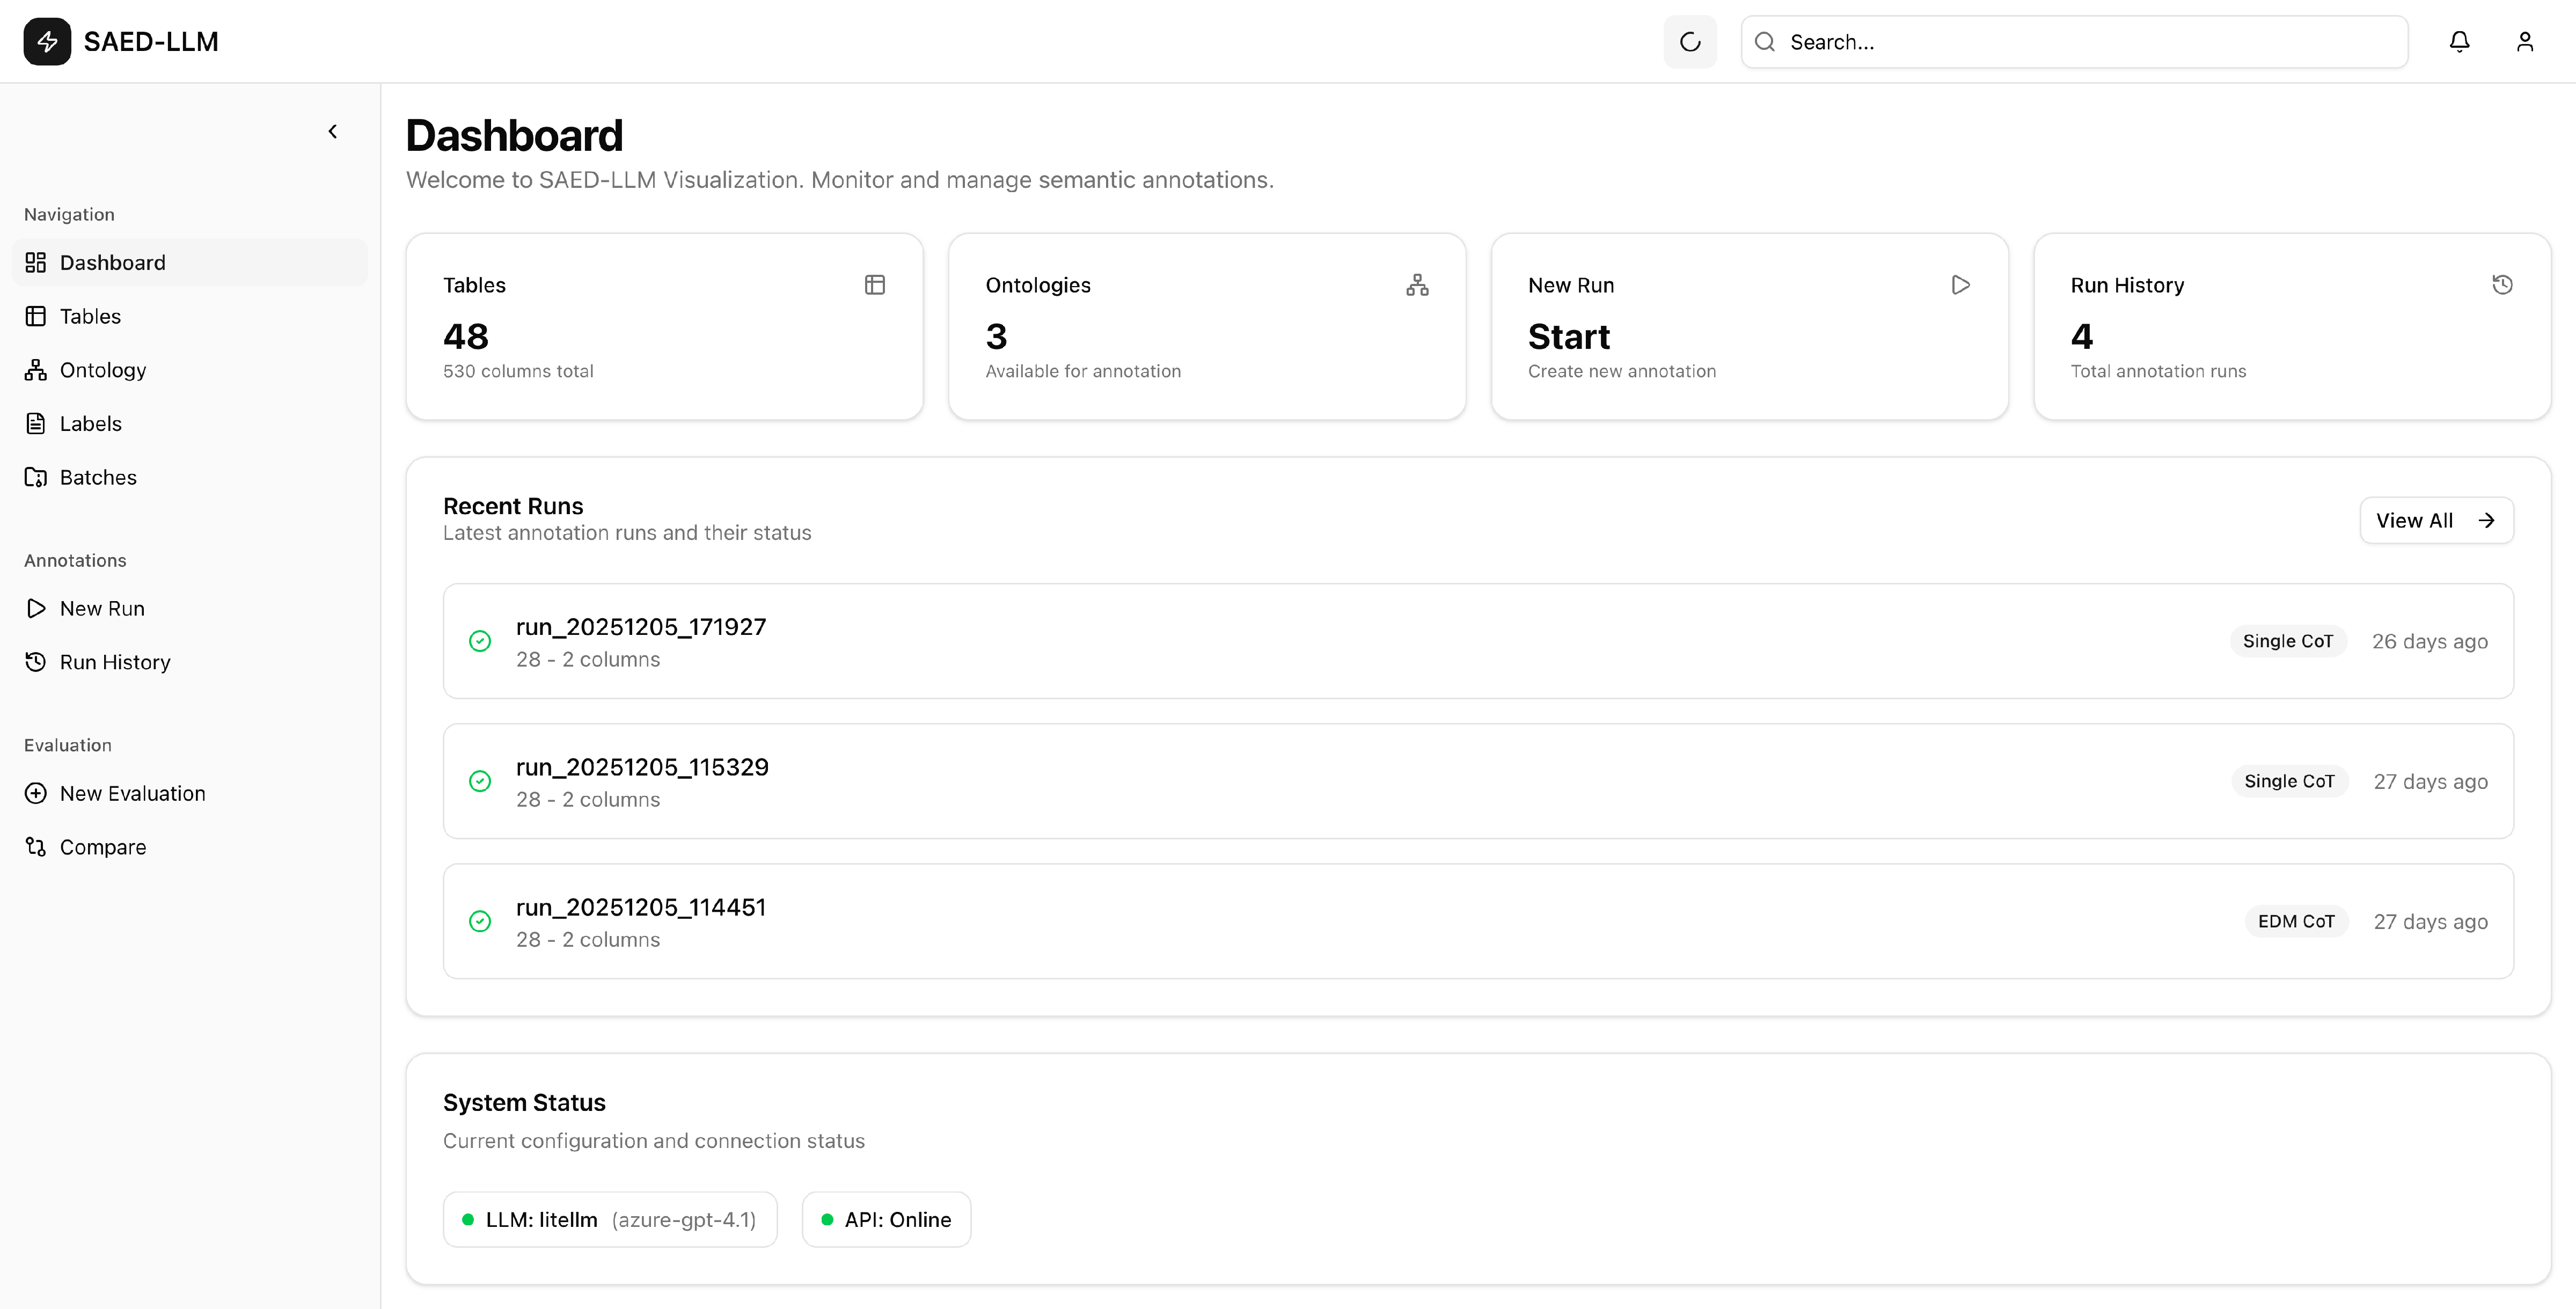
\includegraphics[width=\textwidth]{graphics/canvas/appendix_dashboard.pdf}
    \caption{Dashboard view showing an overview of system status, recent annotation runs, and quick access to main features.}
    \label{fig:webui-dashboard}
\end{figure}

\begin{figure}[htbp]
    \centering
    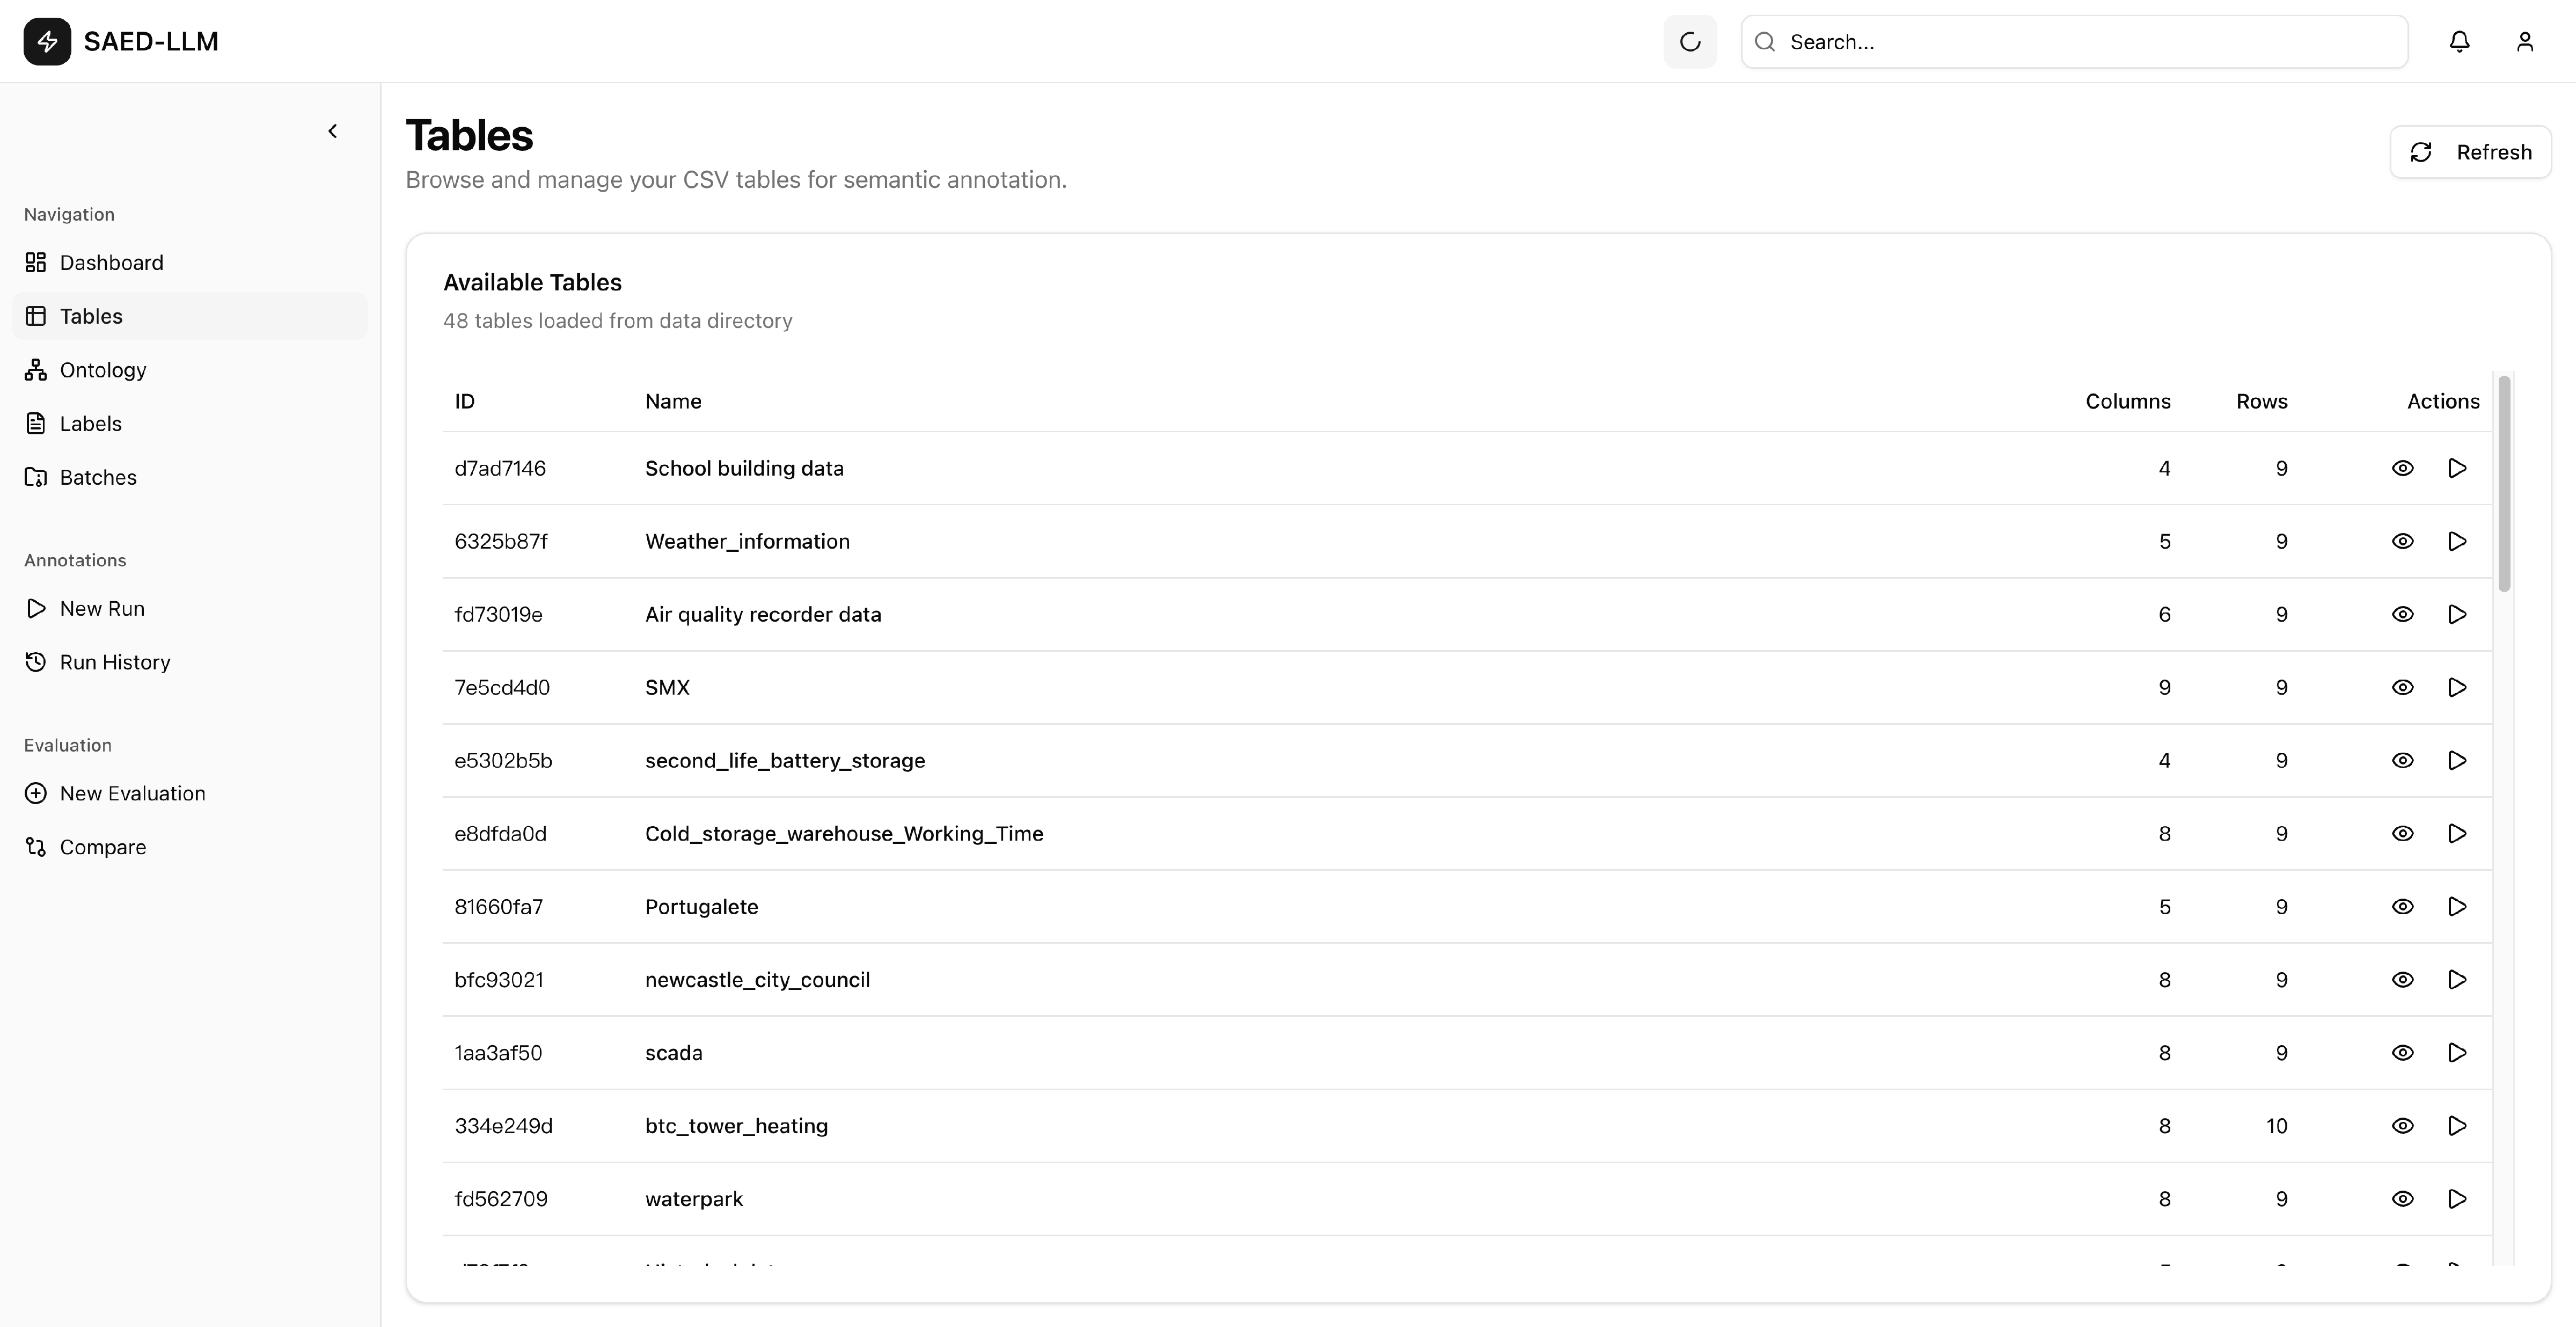
\includegraphics[width=\textwidth]{graphics/canvas/appendix_tables.pdf}
    \caption{Tables management interface for browsing and selecting uploaded CSV files.}
    \label{fig:webui-tables}
\end{figure}

\begin{figure}[htbp]
    \centering
    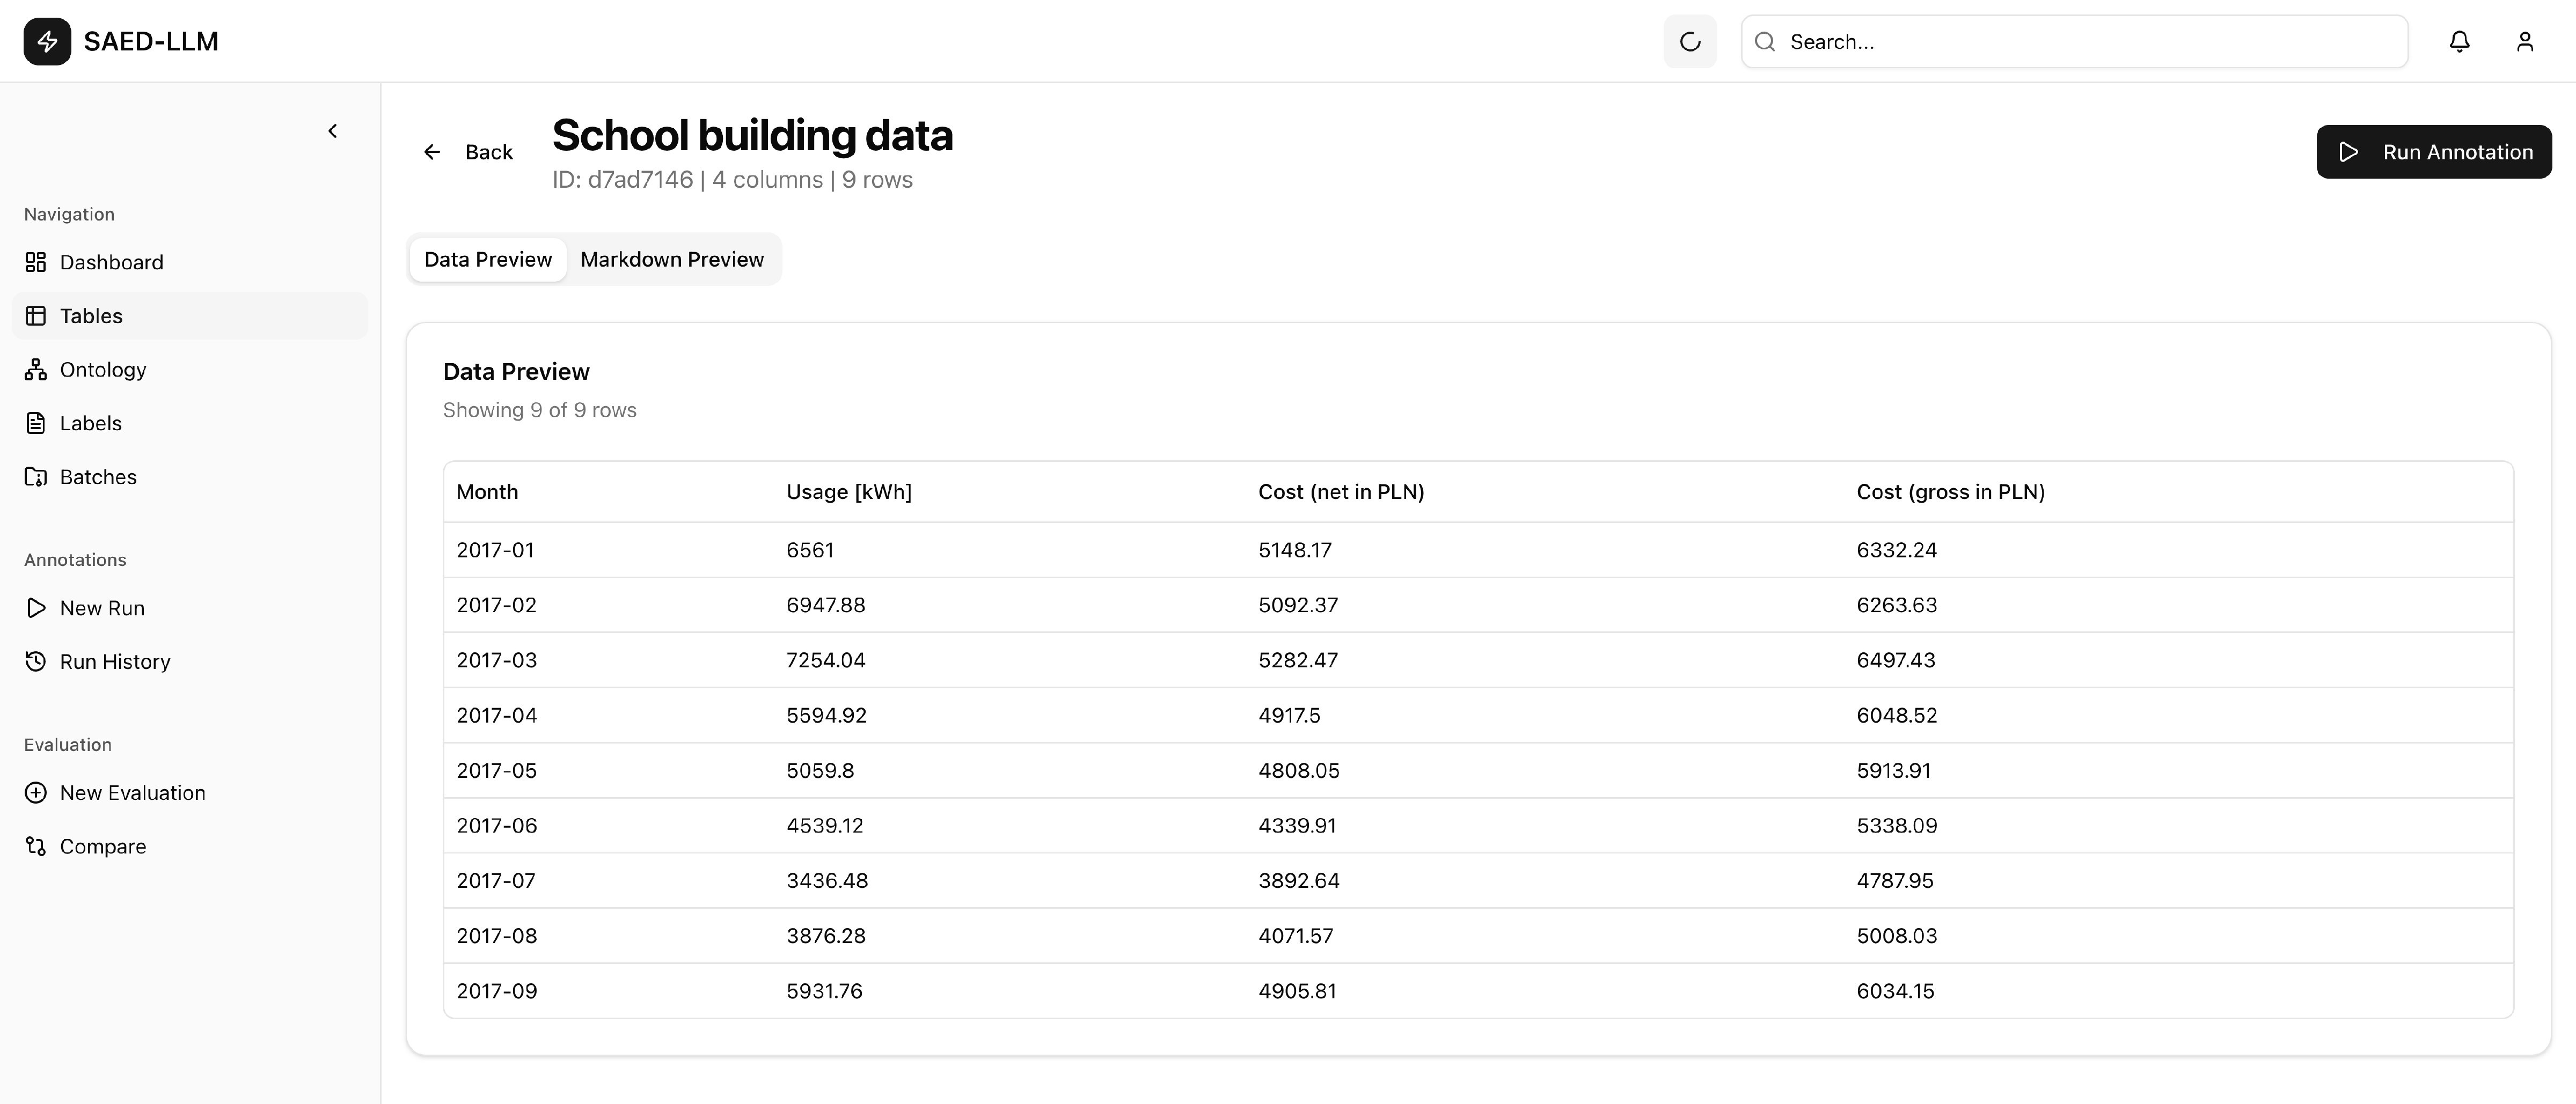
\includegraphics[width=\textwidth]{graphics/canvas/appendix_tables_preview.pdf}
    \caption{Table preview interface displaying column headers and sample data rows.}
    \label{fig:webui-tables-preview}
\end{figure}

\begin{figure}[htbp]
    \centering
    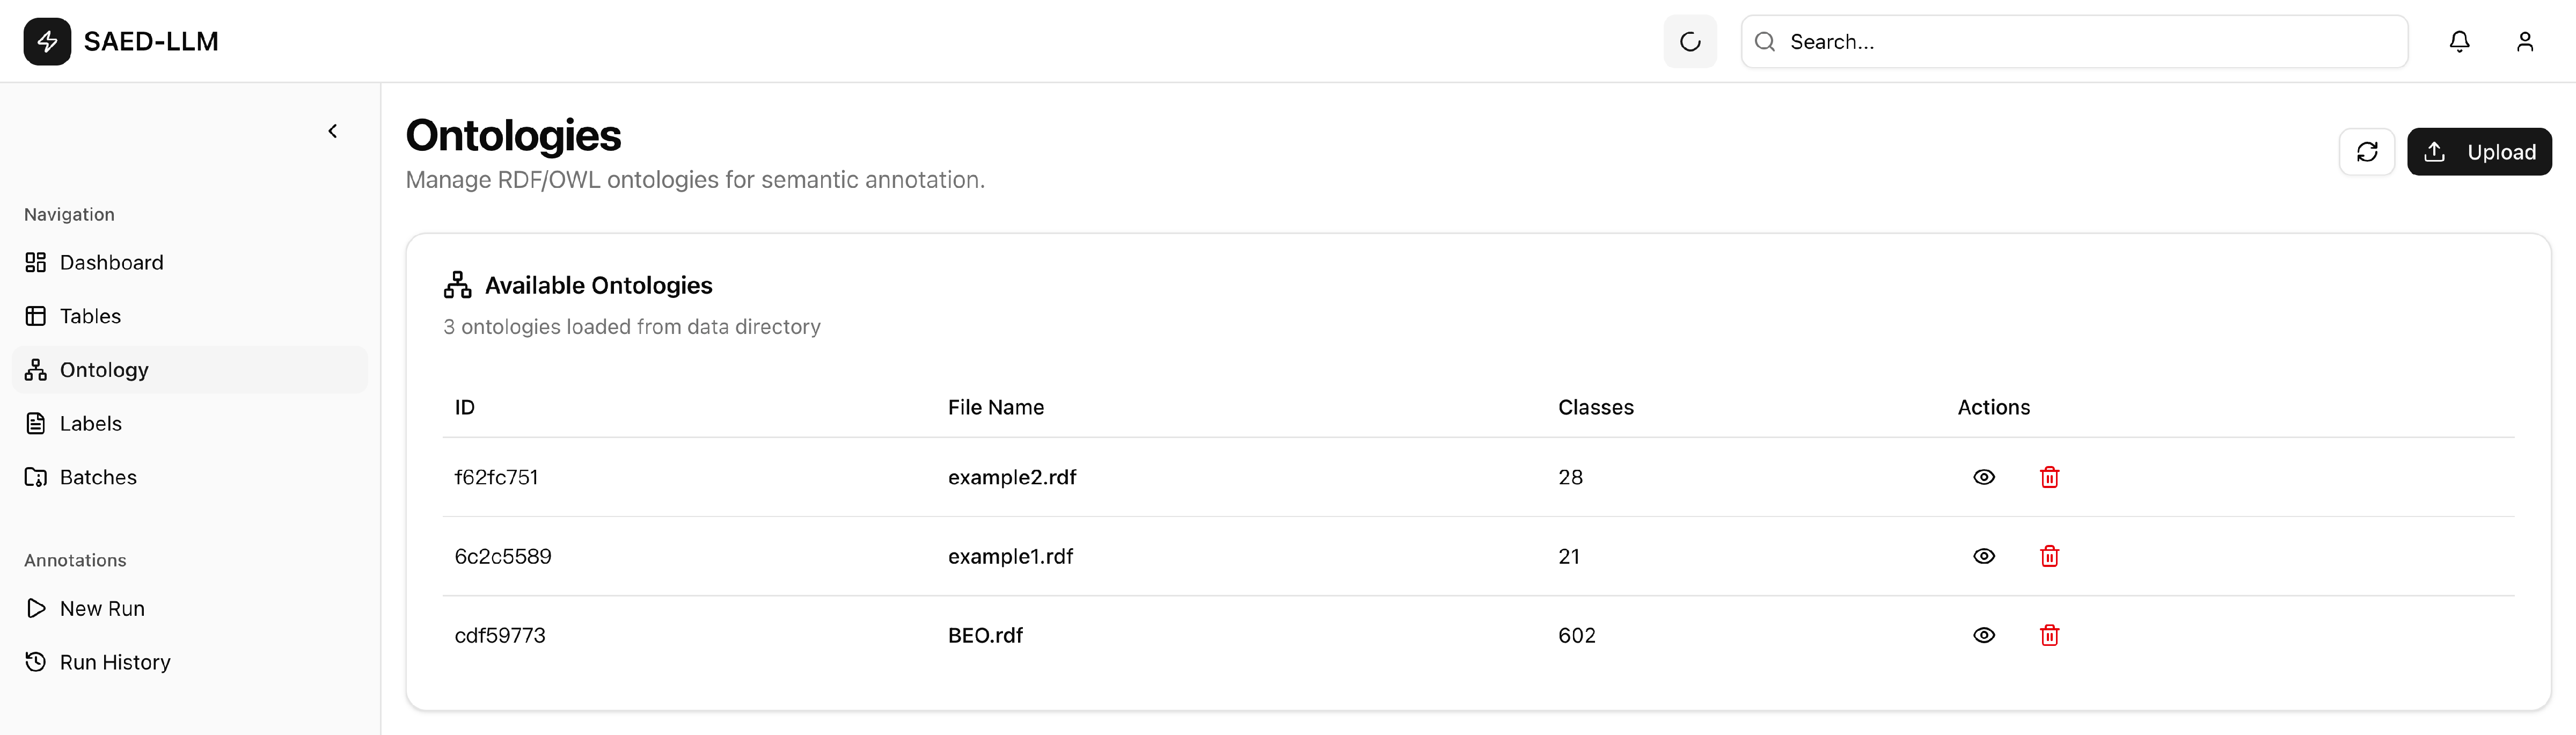
\includegraphics[width=\textwidth]{graphics/canvas/appendix_ontologies.pdf}
    \caption{Ontologies management interface for browsing available ontology files.}
    \label{fig:webui-ontologies}
\end{figure}

\begin{figure}[htbp]
    \centering
    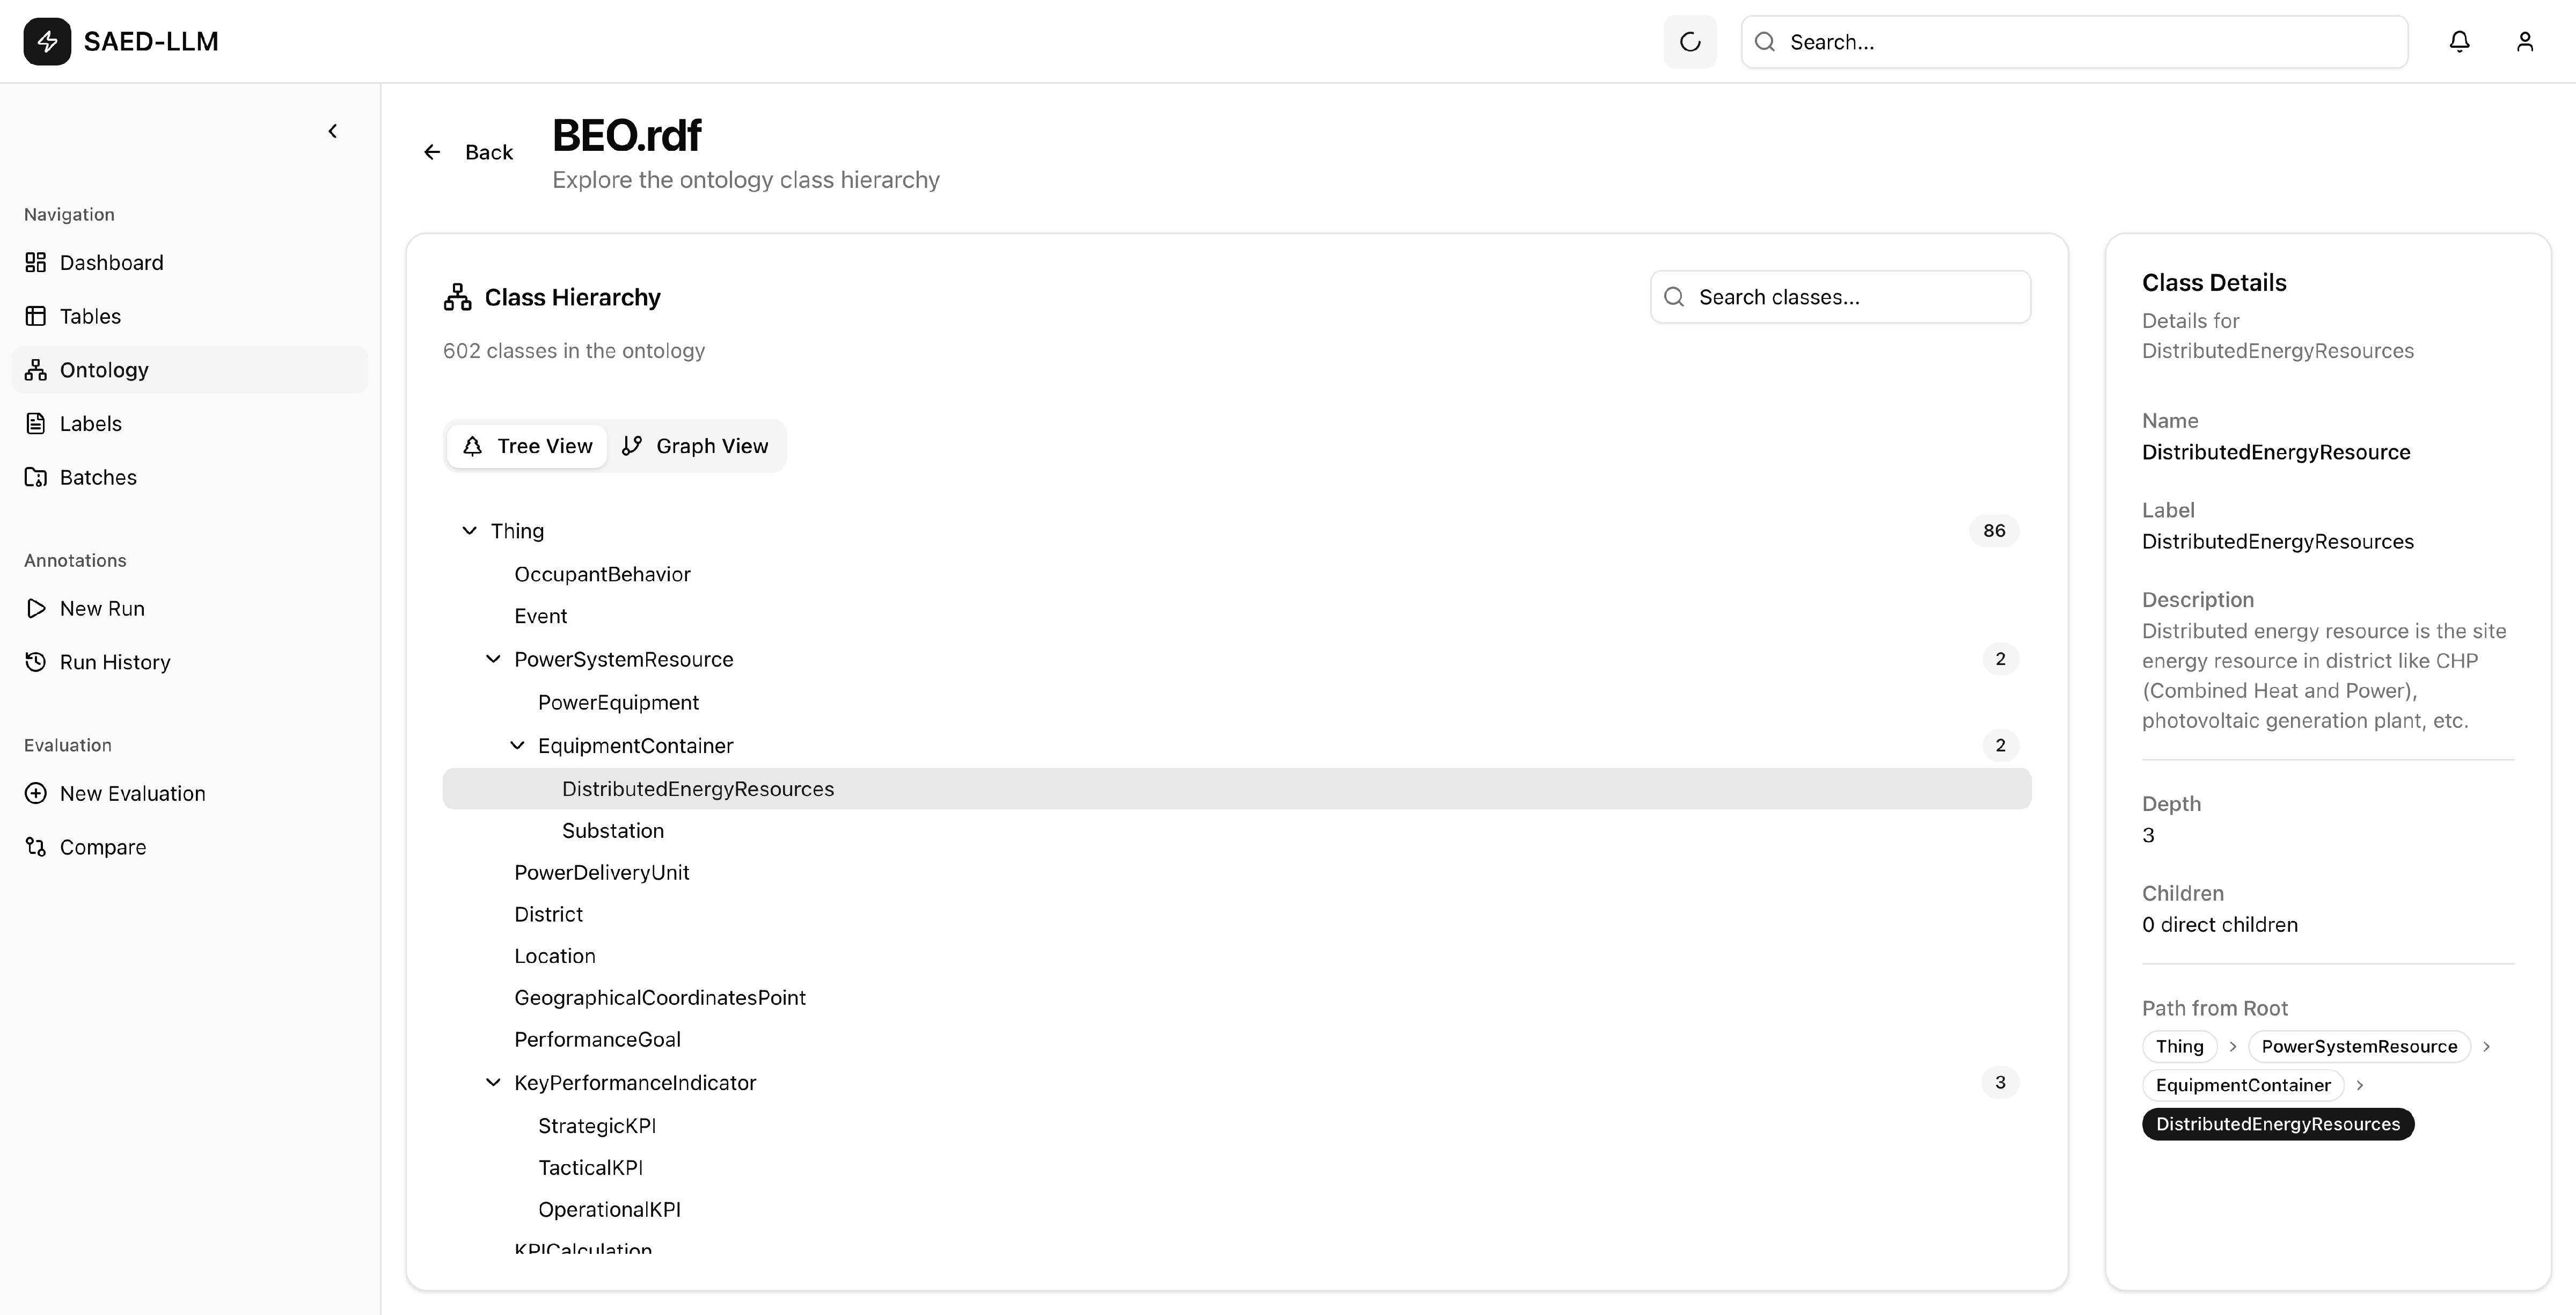
\includegraphics[width=\textwidth]{graphics/canvas/appendix_ontologies_tree_view.pdf}
    \caption{Ontology tree view showing the hierarchical class structure.}
    \label{fig:webui-ontologies-tree}
\end{figure}

\begin{figure}[htbp]
    \centering
    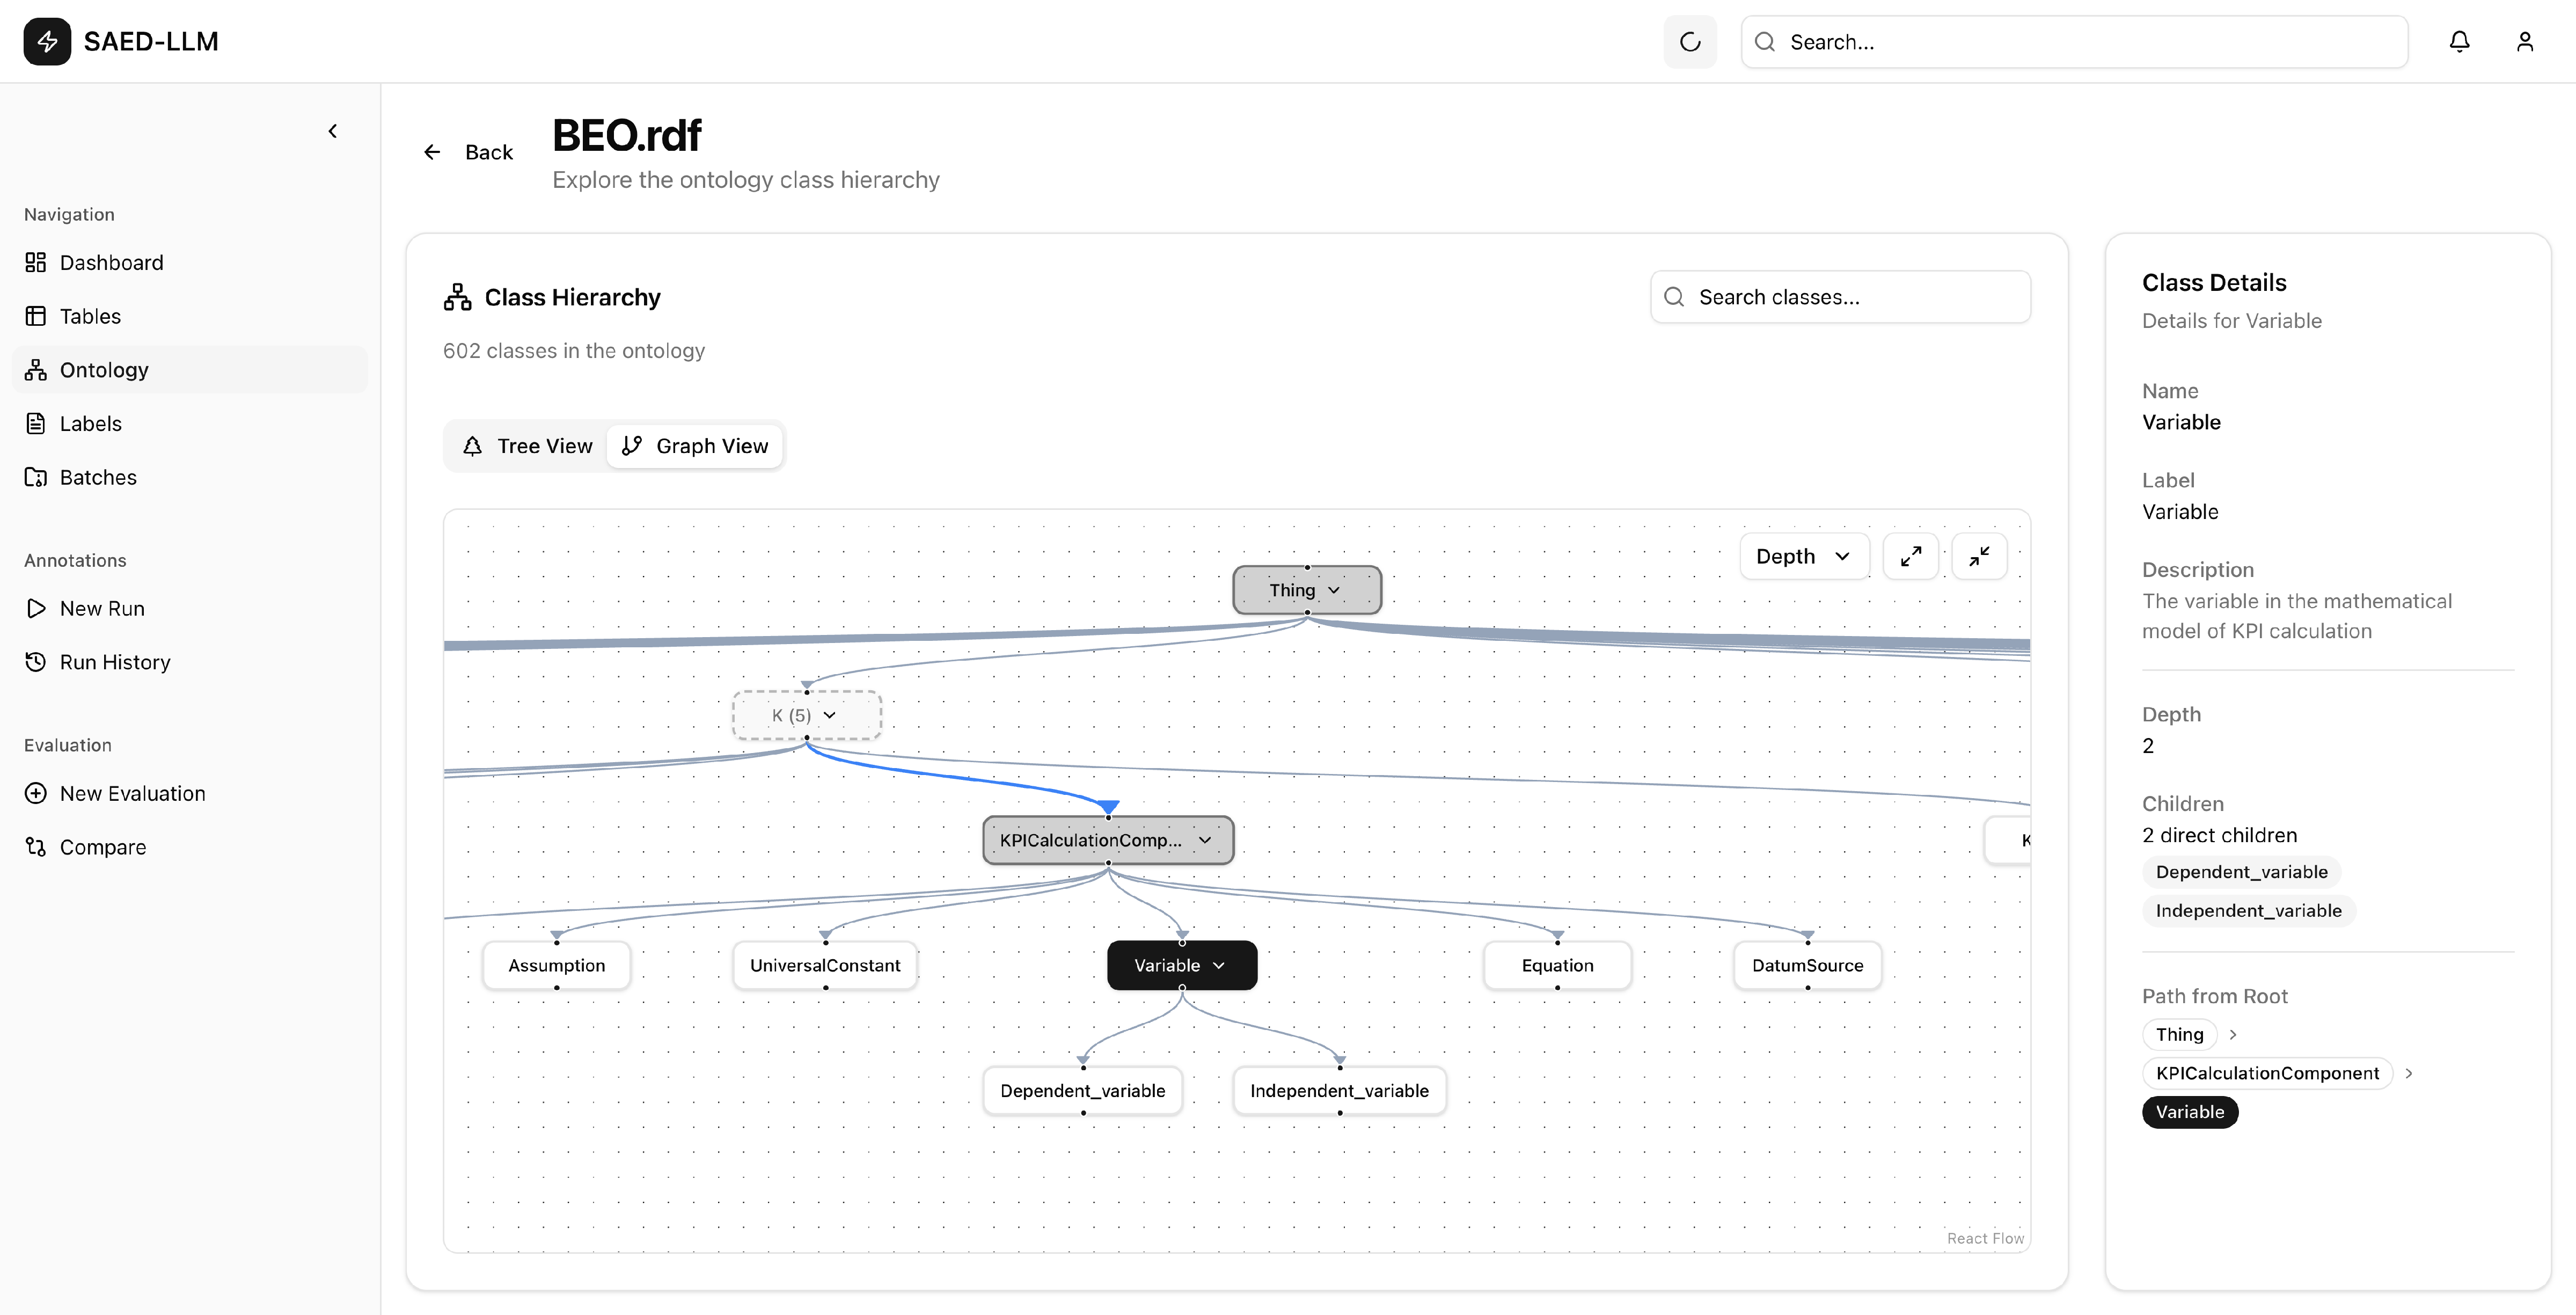
\includegraphics[width=\textwidth]{graphics/canvas/appendix_ontologies_graph_view.pdf}
    \caption{Ontology graph view providing an interactive visualization of class relationships.}
    \label{fig:webui-ontologies-graph}
\end{figure}

\begin{figure}[htbp]
    \centering
    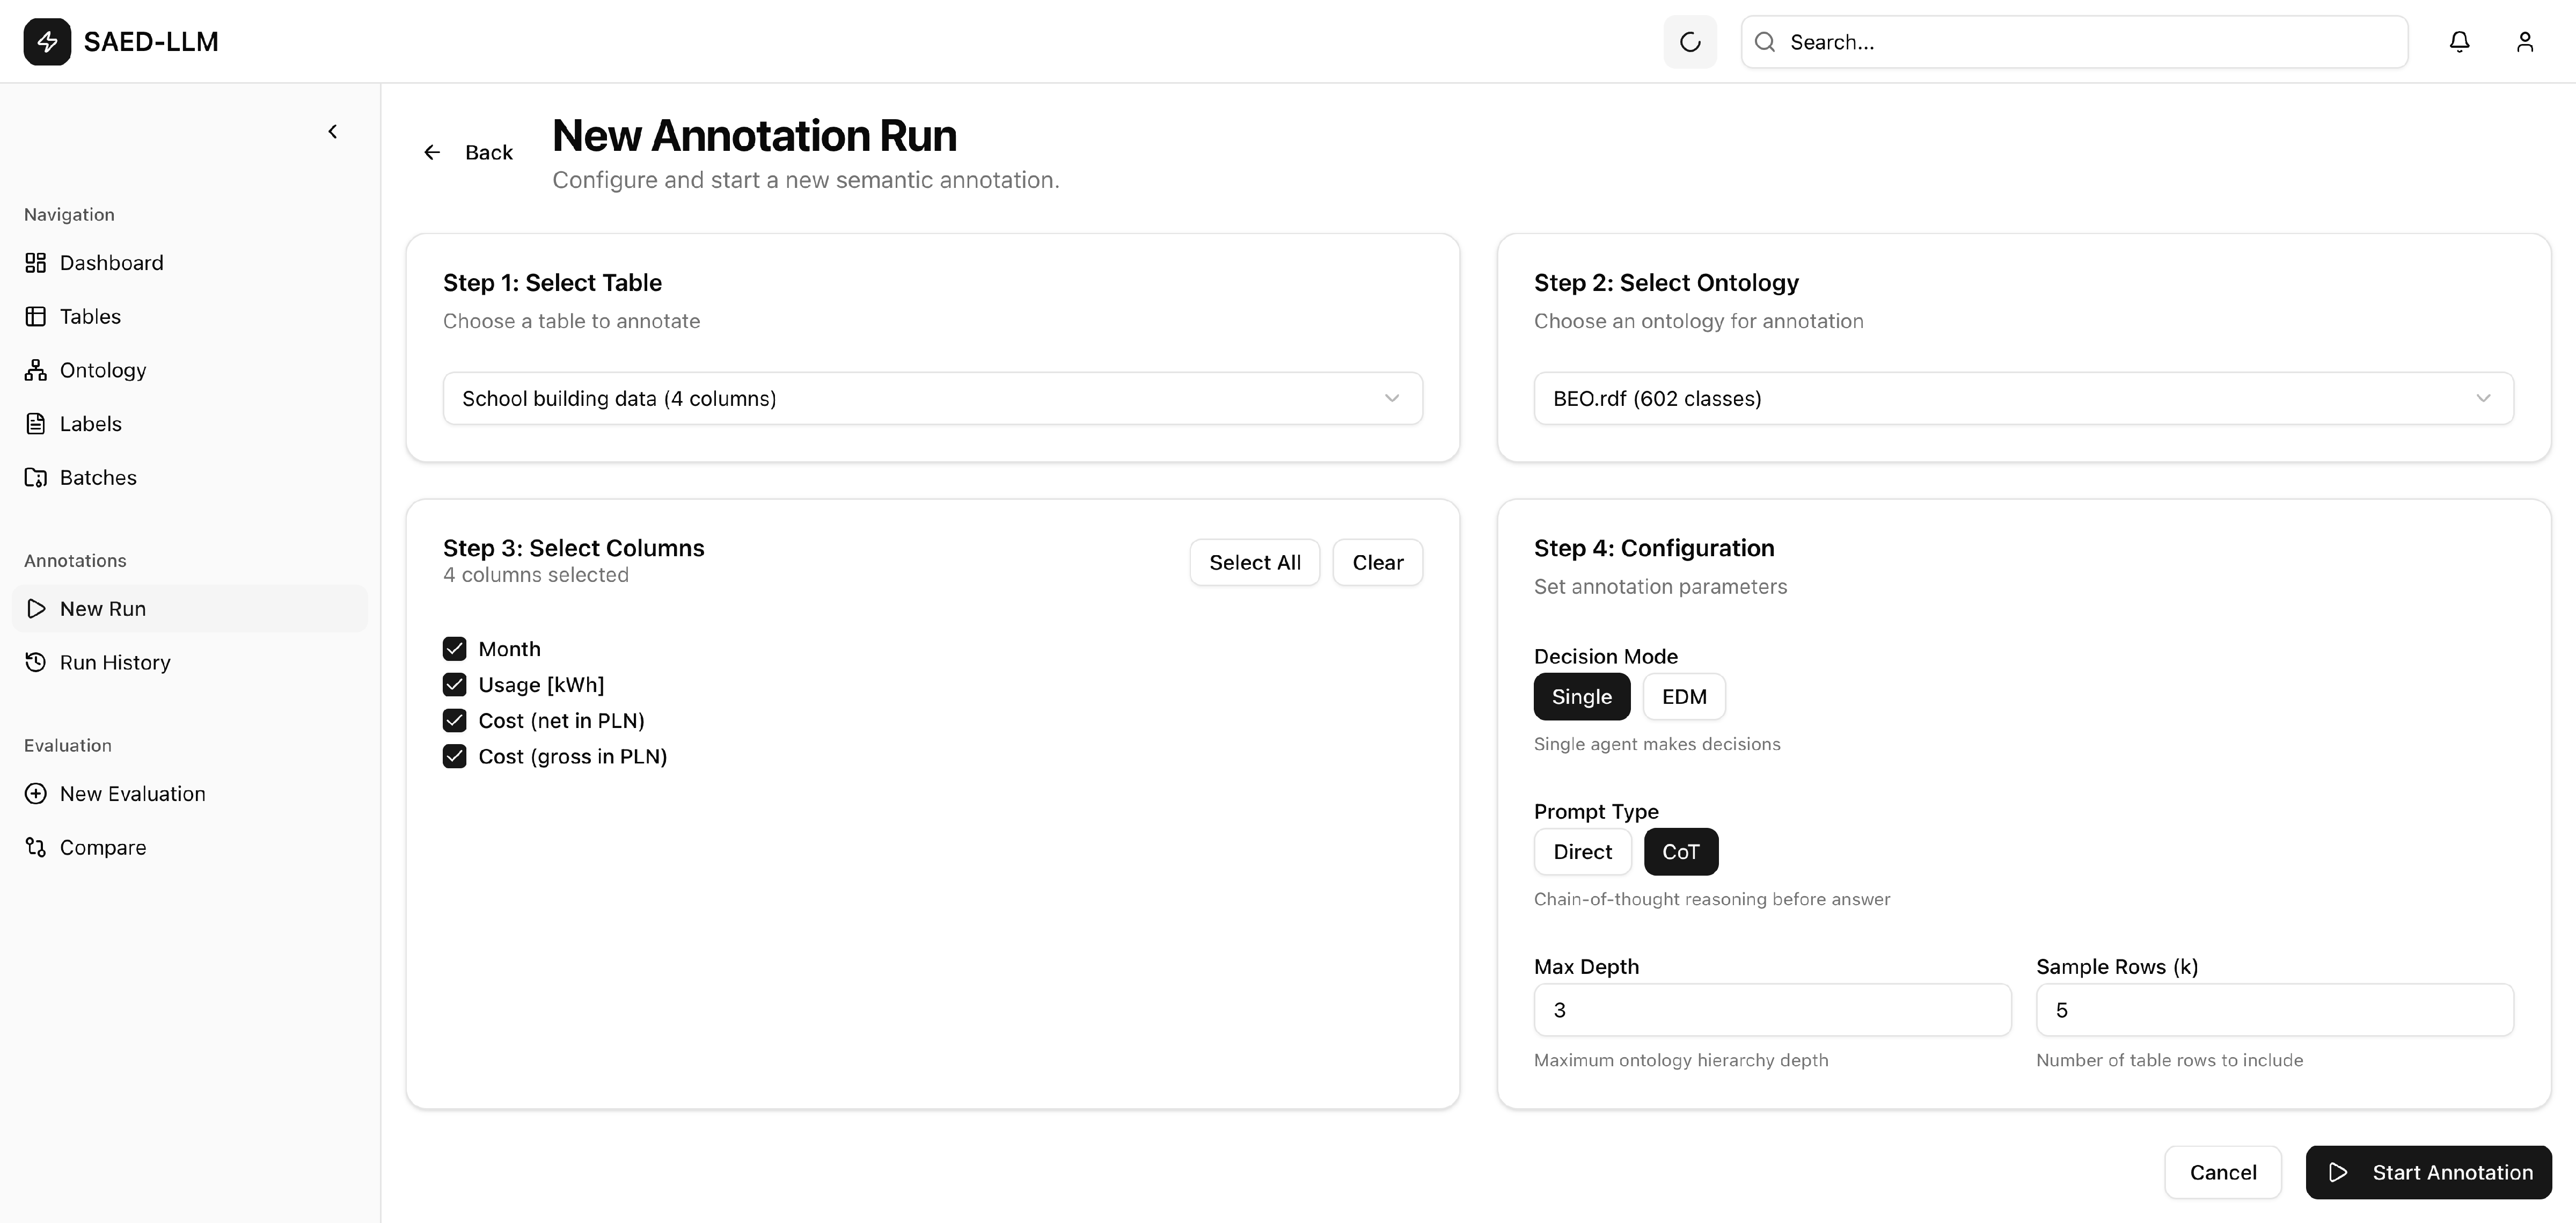
\includegraphics[width=\textwidth]{graphics/canvas/appendix_run.pdf}
    \caption{Annotation run interface showing task configuration and real-time execution progress.}
    \label{fig:webui-run}
\end{figure}

\begin{figure}[htbp]
    \centering
    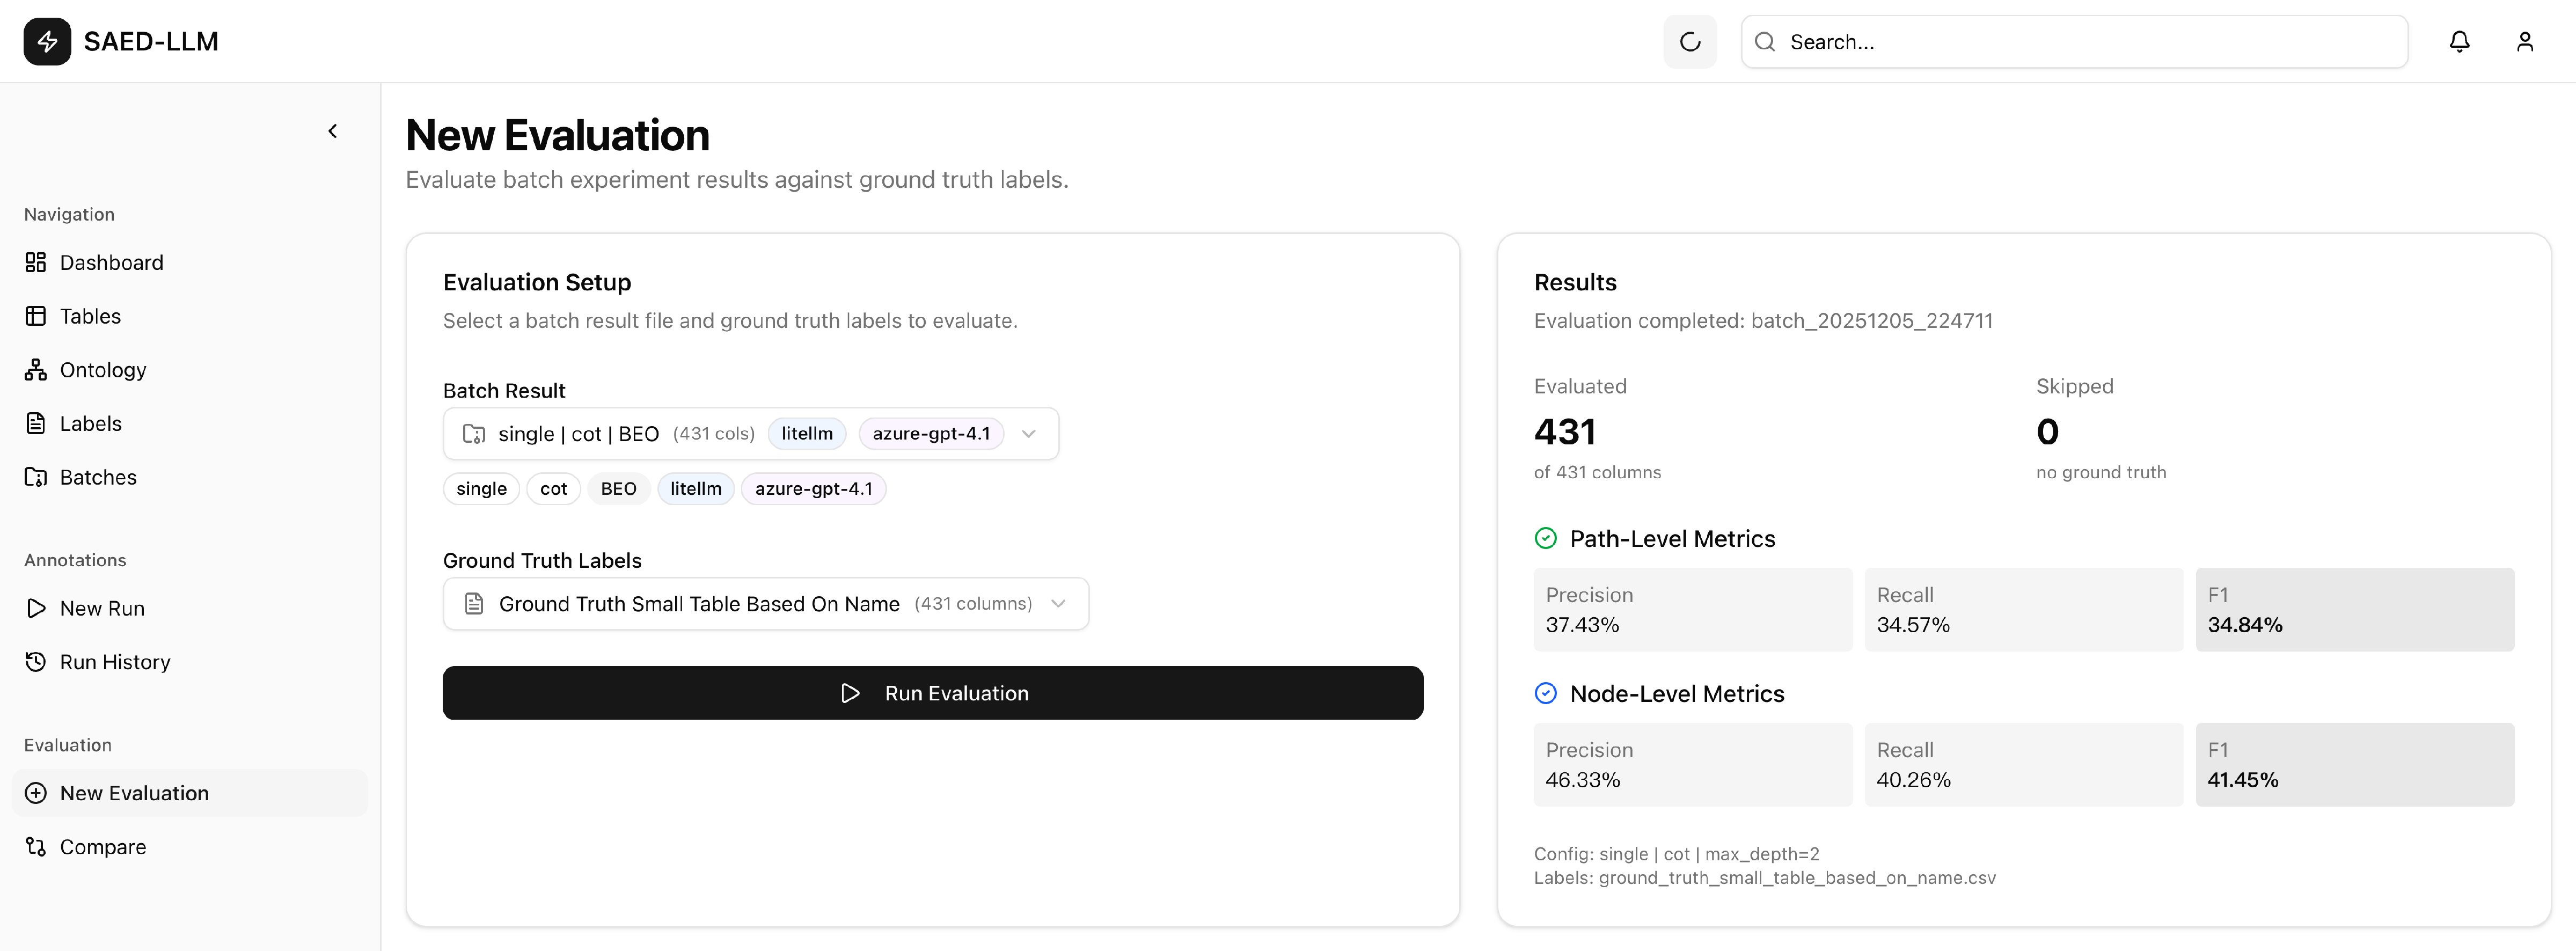
\includegraphics[width=\textwidth]{graphics/canvas/appendix_evaluation.pdf}
    \caption{Evaluation results view displaying annotation accuracy metrics.}
    \label{fig:webui-evaluation}
\end{figure}

\begin{figure}[htbp]
    \centering
    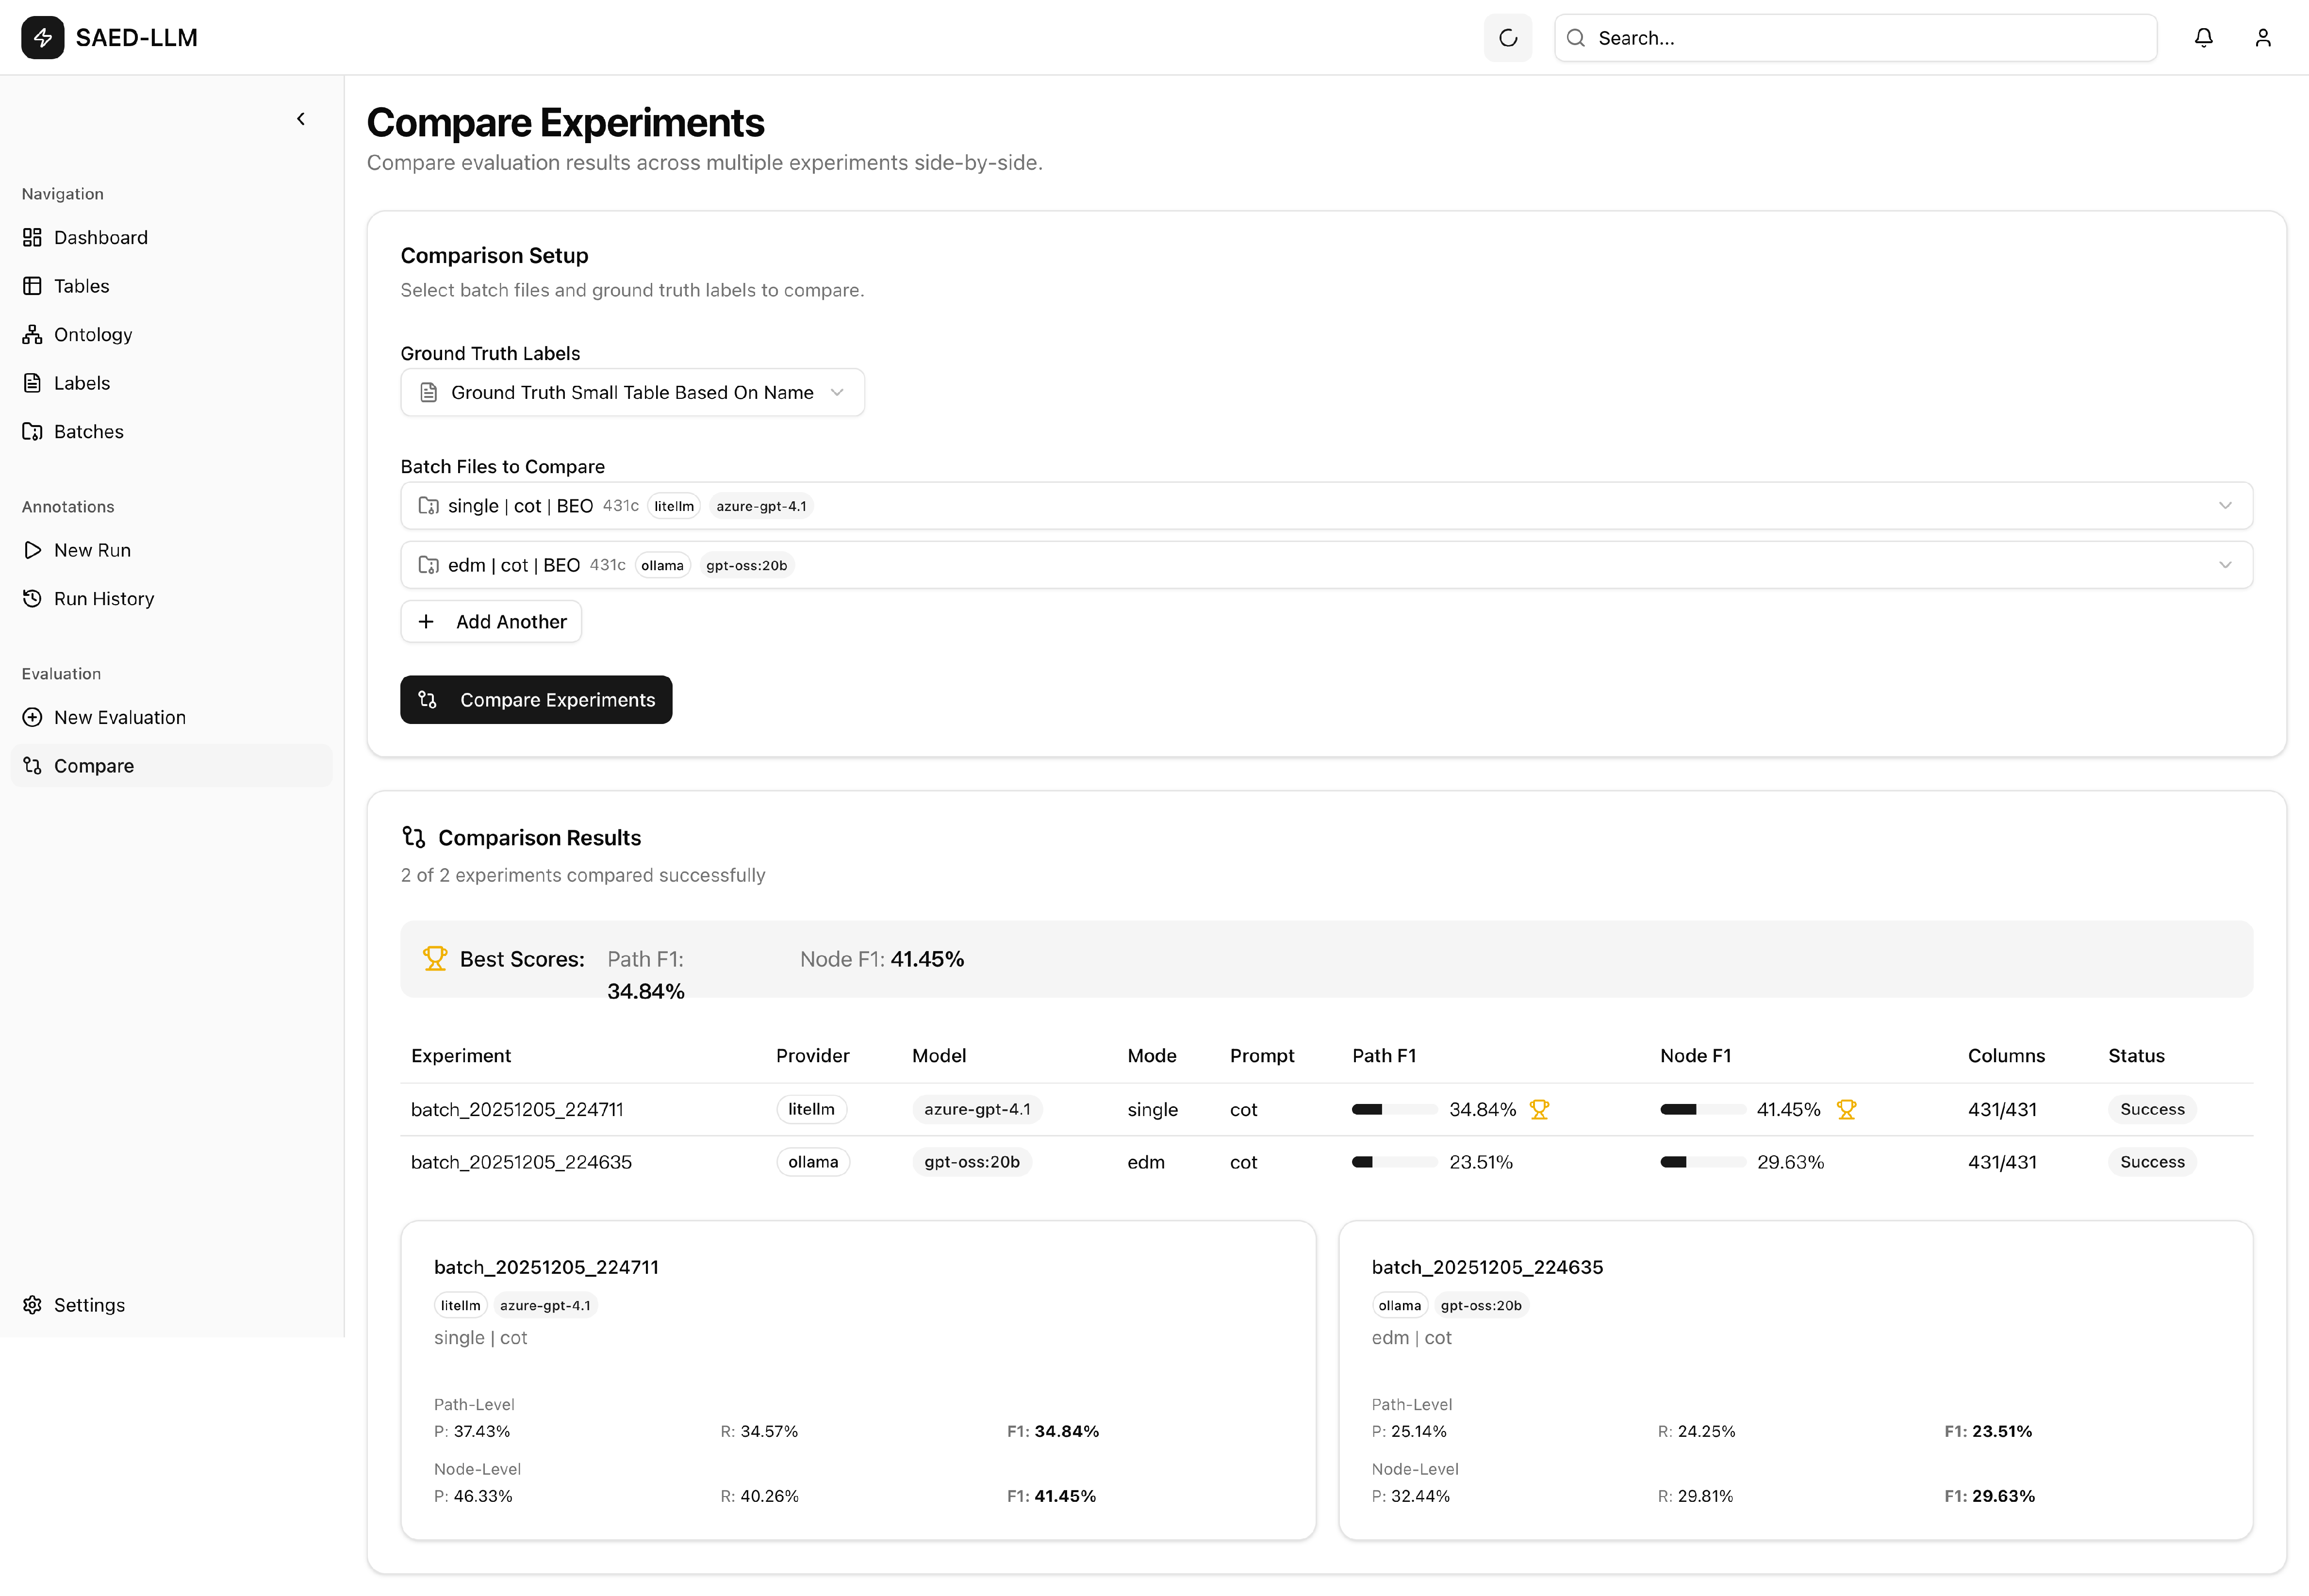
\includegraphics[width=\textwidth]{graphics/canvas/appendix_evaluation_compare.pdf}
    \caption{Evaluation comparison view for analyzing results across different experimental configurations.}
    \label{fig:webui-evaluation-compare}
\end{figure}


\listoffigures
\listoftables
\lstlistoflistings

\end{document}
